% !TeX root = TCC - NetSpot.tex
\documentclass[12pt,a4paper]{article}

% --- PACOTES FUNDAMENTAIS E IDIOMA ---
\usepackage[T1]{fontenc}
\usepackage[utf8]{inputenc}
\usepackage[brazilian]{babel}
\usepackage{mathptmx}
\usepackage{amsmath,amssymb,amsfonts}
\usepackage{geometry}
\geometry{top=3cm,bottom=2cm,left=3cm,right=2cm}
\usepackage{setspace}
\onehalfspacing
\usepackage{graphicx}
\usepackage{float}
\usepackage{booktabs}
\usepackage{array}
\usepackage{longtable}
\usepackage{enumitem}
\usepackage{caption}
\usepackage{titlesec}
\usepackage{fancyhdr}
\usepackage{xcolor}
\usepackage{hyperref}
\usepackage{xurl}
\usepackage[alf,no-abnt-option-file]{abntex2cite}
\usepackage[normalem]{ulem}
\usepackage{indentfirst}
\usepackage{microtype}

% --- CORES E CONFIGURAÇÕES DE LINKS ---
\definecolor{navyblue}{RGB}{15, 44, 89}
\hypersetup{
    colorlinks=true,
    linkcolor=navyblue,
    citecolor=navyblue,
    urlcolor=navyblue,
    pdfauthor={Ronaldo Crispim da Silva Gonçalves},
    pdftitle={Desenvolvimento de um sistema de monitoramento de redes de baixo custo computacional com foco na prevenção de falhas}
}

\graphicspath{{assets/}}
\setlength{\parindent}{1.25cm}
\setlength{\parskip}{0pt}
\setlength{\emergencystretch}{3em}
\captionsetup{font=small,labelfont=normalfont,labelsep=endash,justification=raggedright,singlelinecheck=false}
\renewcommand{\figurename}{Figura}
\renewcommand{\tablename}{Tabela}
\renewcommand{\listfigurename}{LISTA DE ILUSTRAÇÕES}
\renewcommand{\listtablename}{LISTA DE TABELAS}
\renewcommand{\contentsname}{SUMÁRIO}
\renewcommand{\refname}{REFERÊNCIAS}

% --- FORMATAÇÃO DE TÍTULOS CONFORME ABNT ---
\titleformat{\section}{\normalfont\bfseries\normalsize}{\thesection}{0.6em}{\MakeUppercase}
\titleformat{\subsection}{\normalfont\bfseries\normalsize}{\thesubsection}{0.6em}{}
\titleformat{\subsubsection}{\normalfont\bfseries\normalsize}{\thesubsubsection}{0.6em}{}
\titlespacing*{\section}{0pt}{1.5\baselineskip}{1\baselineskip}
\titlespacing*{\subsection}{0pt}{1.5\baselineskip}{1\baselineskip}
\titlespacing*{\subsubsection}{0pt}{1.5\baselineskip}{1\baselineskip}

% --- CABEÇALHOS E RODAPÉS ---
\pagestyle{fancy}
\fancyhf{}
\fancyhead[R]{\thepage}
\renewcommand{\headrulewidth}{0pt}
\setlength{\headheight}{14.5pt}
\setcounter{tocdepth}{2}
\setcounter{secnumdepth}{3}

\newcommand{\fonte}[1]{\par\vspace{-0.5em}{\small Fonte: #1}\par}
\newcommand{\pretextualtitle}[1]{\begin{center}\textbf{\MakeUppercase{#1}}\end{center}\vspace{1em}}

\begin{document}
\sloppy
\hypersetup{pageanchor=false}
\pagenumbering{gobble}

% Capa ABNT
\begin{titlepage}
\begin{center}

\includegraphics[width=3.2cm]{image2.png}\\[0.6cm]
\textbf{MINISTÉRIO DA EDUCAÇÃO}\\
\textbf{INSTITUTO FEDERAL DO NORTE DE MINAS GERAIS -- CAMPUS JANUÁRIA}\\
\textbf{BACHARELADO EM SISTEMAS DE INFORMAÇÃO}

\vfill
\textbf{RONALDO CRISPIM DA SILVA GONÇALVES}

\vfill
\textbf{SISTEMA DE MONITORAMENTO DE REDES DE BAIXO CUSTO COMPUTACIONAL COM FOCO NA PREVENÇÃO DE FALHAS:}\\[0.5em]
\textbf{UMA ABORDAGEM BASEADA EM ANÁLISE DE MÉTRICAS, MONITORAMENTO CONTÍNUO E GERAÇÃO DE ALERTAS PREVENTIVOS EM DISPOSITIVOS CONECTADOS À REDE}

\vfill
\textbf{JANUÁRIA -- MG}\\
2026
\end{center}
\end{titlepage}

% Folha de Rosto ABNT
\begin{titlepage}
\begin{center}
\textbf{RONALDO CRISPIM DA SILVA GONÇALVES}

\vfill
\textbf{SISTEMA DE MONITORAMENTO DE REDES DE BAIXO CUSTO COMPUTACIONAL COM FOCO NA PREVENÇÃO DE FALHAS:}\\[0.5em]
\textbf{UMA ABORDAGEM BASEADA EM ANÁLISE DE MÉTRICAS, MONITORAMENTO CONTÍNUO E GERAÇÃO DE ALERTAS PREVENTIVOS EM DISPOSITIVOS CONECTADOS À REDE}
\end{center}

\vfill
\begin{flushright}
\begin{minipage}{0.52\textwidth}
\singlespacing
Trabalho de Conclusão de Curso apresentado ao Instituto Federal do Norte de Minas Gerais (IFNMG) -- Campus Januária, como requisito parcial para obtenção do título de Bacharel em Sistemas de Informação.

\vspace{0.8em}
Prof. Orientador: MSc. Adriano Antunes Prates\\
Área de conhecimento: Ciência da Computação
\end{minipage}
\end{flushright}

\vfill
\begin{center}
\textbf{JANUÁRIA -- MG}\\
2026
\end{center}
\end{titlepage}

% Folha de Aprovação ABNT
\clearpage
\thispagestyle{empty}
\begin{center}
\textbf{RONALDO CRISPIM DA SILVA GONÇALVES}

\vspace{1.5em}
\textbf{SISTEMA DE MONITORAMENTO DE REDES DE BAIXO CUSTO COMPUTACIONAL COM FOCO NA PREVENÇÃO DE FALHAS}
\end{center}

\vspace{1.5em}
\begin{flushright}
\begin{minipage}{0.52\textwidth}
\singlespacing
Trabalho de Conclusão de Curso aprovado pela Banca Examinadora como requisito parcial para obtenção do título de Bacharel em Sistemas de Informação do Instituto Federal do Norte de Minas Gerais (IFNMG) -- Campus Januária.
\end{minipage}
\end{flushright}

\vspace{2em}
\noindent Aprovado em: \underline{\hspace{1.5cm}} de \underline{\hspace{3.5cm}} de 2026.

\vfill
\begin{center}
\textbf{BANCA EXAMINADORA}

\vspace{2.5em}
\rule{11cm}{0.4pt}\\
Prof. MSc. Adriano Antunes Prates -- Orientador\\
IFNMG -- Campus Januária

\vspace{2.5em}
\rule{11cm}{0.4pt}\\
Prof. Membro da Banca Examinadora\\
IFNMG -- Campus Januária

\vspace{2.5em}
\rule{11cm}{0.4pt}\\
Prof. Membro da Banca Examinadora\\
IFNMG -- Campus Januária
\end{center}
\vfill
\clearpage

% Dedicatória
\thispagestyle{empty}
\vspace*{0.60\textheight}
\begin{flushright}
\begin{minipage}{0.52\textwidth}
Dedico este trabalho aos meus pais, ao professor Raphael Hoed e ao meu orientador Adriano Antunes; é graças ao esforço de todos que hoje posso concluir essa trajetória e finalizar o curso.\end{minipage}
\end{flushright}
\clearpage

% Agradecimentos
\pretextualtitle{AGRADECIMENTOS}
A Deus, por ter permitido que eu tivesse saúde e determinação para não desanimar durante a realização deste trabalho.

Aos meus pais e irmãos, que me incentivaram nos momentos difíceis e compreenderam a minha ausência enquanto eu me dedicava à realização deste trabalho.

Aos professores, pelas correções e ensinamentos que me permitiram apresentar um melhor desempenho no meu processo de formação profissional ao longo do curso.

A todos que participaram, direta ou indiretamente do desenvolvimento deste trabalho de pesquisa, enriquecendo o meu processo de aprendizado.

Ao Instituto Federal do Norte de Minas Gerais (IFNMG), essencial no meu processo de formação profissional, pela dedicação e por tudo o que aprendi ao longo dos anos do curso.

\clearpage

% Epígrafe
\thispagestyle{empty}
\vspace*{0.58\textheight}
\begin{flushright}
\begin{minipage}{0.52\textwidth}
\begin{flushright}
``Educação não transforma o mundo.\\
Educação muda as pessoas.\\
Pessoas mudam o mundo.''\\[0.8em]
(Paulo Freire)
\end{flushright}
\end{minipage}
\end{flushright}
\clearpage

% Resumo
\pretextualtitle{RESUMO}
Com a crescente expansão da conectividade, garantir a disponibilidade e o desempenho dos serviços de rede tornou-se indispensável. Em ambientes de pequeno e médio porte, as soluções tradicionais de gerenciamento frequentemente impõem barreiras operacionais severas devido à sua elevada complexidade de instalação, necessidade de manutenção contínua e curvas de aprendizado íngremes. Este trabalho apresenta o desenvolvimento e a validação do \textbf{NetSpot (NOC Lite)}, uma solução de monitoramento de redes concebida com ênfase na praticidade operacional, simplicidade de implantação e baixo custo computacional, voltada à detecção proativa e preventiva de falhas. O sistema adota uma Arquitetura Orientada a Eventos (EDA) e princípios de \textit{Clean Architecture}, estruturada em 5 microsserviços containerizados prontos para execução (\textit{turn-key}) via Docker (FastAPI, PostgreSQL 15, RabbitMQ 3, N8N Automation e Nginx Alpine). O motor de coleta assíncrono em Python (3.11/3.12) executa verificações multi-protocolo (ICMP, TCP, HTTP/HTTPS, DNS e SNMP multivendor para MIBs Linux e Windows), alimentando um barramento RabbitMQ com tolerância a falhas via \textit{Dead Letter Queue} (DLQ) e mecanismos de \textit{Circuit Breaker}, \textit{Anti-Spam} e \textit{Graceful Shutdown}. As métricas alimentam o cálculo contínuo do \textit{Health Score} (0 a 100\%), Disponibilidade geral (SLA calculado via União de Intervalos), \textit{Jitter} e tendência de instabilidade, despachando alertas preventivos formatados para o Telegram via N8N. A visualização ocorre em uma interface SPA moderna, ergonômica e intuitiva, com suporte a temas \textit{Dark and White}, conformidade de acessibilidade digital (WCAG 2.1 AA) e atualização otimizada. A validação técnica foi realizada em ambiente simulado no framework Kathará (topologia padrão com 40 nós roteados e topologia de estresse em alta densidade com 126 nós monitorados), nos computadores físicos dos laboratórios do IFNMG e através de uma suíte de 86 testes automatizados (100\% de aprovação em Pytest), comprovando o consumo reduzido de CPU ($<$ 10\%), a resposta ágil a anomalias e a facilidade de uso do sistema.

\vspace{1em}
\noindent\textbf{Palavras-chave:} Monitoramento de rede. NOC Lite. Praticidade operacional. Arquitetura orientada a eventos. Prevenção de falhas. Health Score. NetSpot.
\clearpage

% Abstract
\pretextualtitle{ABSTRACT}
With the growing expansion of connectivity, ensuring the availability and performance of network services has become indispensable. In small- and medium-sized environments, traditional network management solutions often impose severe operational barriers due to high configuration complexity, continuous maintenance demands, and steep learning curves. This work presents the development and validation of \textbf{NetSpot (NOC Lite)}, a network monitoring solution designed with an emphasis on operational simplicity, turnkey deployment, and low computational cost, focused on proactive and preventive failure detection. The system adopts an Event-Driven Architecture (EDA) and Clean Architecture principles, organized into 5 containerized microservices managed via Docker (FastAPI, PostgreSQL 15, RabbitMQ 3, N8N Automation, and Nginx Alpine). The asynchronous Python (3.11/3.12) collection engine performs multi-protocol checks (ICMP, TCP, HTTP/HTTPS, DNS, and multivendor SNMP for Linux and Windows MIBs), feeding a RabbitMQ message broker with fault tolerance provided by a Dead Letter Queue (DLQ) and Circuit Breaker, Anti-Spam, and Graceful Shutdown mechanisms. The collected telemetry supports the continuous statistical calculation of the Health Score (0 to 100\%), overall availability (SLA computed via Interval Merging), Jitter, and instability trends, dispatching formatted preventive alerts to Telegram via N8N. Data visualization is delivered through a modern, ergonomic, and intuitive SPA interface featuring Dark and White themes, digital accessibility compliance (WCAG 2.1 AA), and optimized UI rendering. Technical validation was conducted in a simulated environment using the Kathará framework (standard 40-node routed topology and scaled high-density stress topology with 126 monitored nodes), on physical workstations at IFNMG laboratories, and through a suite of 86 automated tests (100\% passed in Pytest), demonstrating low CPU consumption ($<$ 10\%), rapid incident response, and high operational usability.

\vspace{1em}
\noindent\textbf{Keywords:} Network monitoring. NOC Lite. Operational simplicity. Event-driven architecture. Failure prevention. Health Score. NetSpot.
\clearpage

\listoffigures
\clearpage
\listoftables
\clearpage

\pretextualtitle{LISTA DE ABREVIATURAS E SIGLAS}
\begin{longtable}{@{}>{\bfseries}p{2.2cm}p{11.5cm}@{}}
AMQP & Advanced Message Queuing Protocol \\
API & Application Programming Interface \\
ARIA & Accessible Rich Internet Applications \\
ARP & Address Resolution Protocol \\
ASGI & Asynchronous Server Gateway Interface \\
BNDES & Banco Nacional de Desenvolvimento Econômico e Social \\
Bps & Bytes per Second \\
CIDR & Classless Inter-Domain Routing \\
CPU & Central Processing Unit \\
CSS & Cascading Style Sheets \\
DCP & Diagrama de Classes de Projeto \\
DHCP & Dynamic Host Configuration Protocol \\
DLQ & Dead Letter Queue \\
DLX & Dead Letter Exchange \\
DNS & Domain Name System \\
DOM & Document Object Model \\
DSR & Design Science Research \\
DSS & Diagrama de Sequência de Sistema \\
DTO & Data Transfer Object \\
EDA & Event-Driven Architecture \\
ES6 & ECMAScript 2015 (6ª Edição) \\
FURPS+ & Funcionalidade, Usabilidade, Confiabilidade, Desempenho e Suportabilidade \\
GRASP & General Responsibility Assignment Software Patterns \\
HTML & HyperText Markup Language \\
HTML5 & HyperText Markup Language versão 5 \\
HTTP & HyperText Transfer Protocol \\
HTTPS & HyperText Transfer Protocol Secure \\
ICMP & Internet Control Message Protocol \\
IFNMG & Instituto Federal do Norte de Minas Gerais \\
IoT & Internet of Things \\
IP & Internet Protocol \\
ISO & International Organization for Standardization \\
ITIL & Information Technology Infrastructure Library \\
JS & JavaScript \\
JWT & JSON Web Token \\
KPI & Key Performance Indicator \\
LAN & Local Area Network \\
LTS & Long Term Support \\
MIB & Management Information Base \\
MIME & Multipurpose Internet Mail Extensions \\
MTTR & Mean Time to Repair (Tempo Médio de Reparo) \\
NAT & Network Address Translation \\
NOC & Network Operations Center \\
OCL & Object Constraint Language \\
OID & Object Identifier \\
OLS & Ordinary Least Squares \\
ORM & Object-Relational Mapping \\
OSI & Open Systems Interconnection \\
OWASP & Open Web Application Security Project \\
PDU & Protocol Data Unit \\
POSIX & Portable Operating System Interface \\
QoS & Quality of Service \\
RAM & Random Access Memory \\
RBAC & Role-Based Access Control \\
REST & Representational State Transfer \\
RFC & Request for Comments \\
RLS & Row Level Security \\
SGBD & Sistema Gerenciador de Banco de Dados \\
SLA & Service Level Agreement \\
SNMP & Simple Network Management Protocol \\
SOLID & Princípios de Design Orientado a Objetos (SRP, OCP, LSP, ISP, DIP) \\
SPA & Single Page Application \\
SVG & Scalable Vector Graphics \\
TCP & Transmission Control Protocol \\
TI & Tecnologia da Informação \\
TIC & Tecnologia da Informação e Comunicação \\
UDP & User Datagram Protocol \\
UI & User Interface \\
UML & Unified Modeling Language \\
UTC & Coordinated Universal Time (Tempo Universal Coordenado) \\
UUID & Universally Unique Identifier \\
UX & User Experience \\
WAI-ARIA & Web Accessibility Initiative -- Accessible Rich Internet Applications \\
WCAG & Web Content Accessibility Guidelines \\
W3C & World Wide Web Consortium \\
XSS & Cross-Site Scripting \\
\end{longtable}
\clearpage

\tableofcontents
\clearpage
\hypersetup{pageanchor=true}
\pagenumbering{arabic}
\setcounter{page}{1}

\section{INTRODUÇÃO}
As redes de computadores desempenham um papel fundamental na sociedade moderna, sustentando desde comunicações pessoais até operações críticas em setores econômicos, governamentais e educacionais. Nesse contexto, a disponibilidade, o desempenho e a confiabilidade das redes tornam-se fatores essenciais para garantir a continuidade dos serviços e a eficiência das operações.

Nesse cenário, problemas relacionados ao congestionamento, latência, perda de pacotes e outras métricas que impactam o tráfego da rede exemplificam como a gestão de desempenho está intrinsecamente ligada à gestão de falhas, uma vez que ambas visam monitorar e controlar os ativos para assegurar sua operação eficiente \cite{silva2024zabbix}. Contudo, um dos principais desafios na gerência atual refere-se à crescente diversidade de dispositivos e softwares de Tecnologia da Informação e Comunicação (TIC), impulsionada pela expansão de tecnologias em nuvem, redes móveis e ambientes heterogêneos \cite{basso2020administracao}.

Diante desse contexto, este trabalho aborda a seguinte questão central de pesquisa: \textbf{Como identificar falhas e degradações de desempenho em dispositivos conectados antes que elas afetem a disponibilidade dos serviços, mantendo um baixo custo computacional e operacional?}

A hipótese que norteou o desenvolvimento deste estudo é que a implementação de um sistema de monitoramento pautado em uma Arquitetura Orientada a Eventos (EDA) assíncrona, combinada com mecanismos inteligentes de autocura (\textit{Self-Healing}) e desativação temporária de \textit{polling} (\textit{Circuit Breaker}), permite detectar anomalias e emitir alertas preventivos antecipadamente, reduzindo drasticamente o \textit{overhead} computacional em comparação às abordagens tradicionais de \textit{polling} síncrono e relacional.

Para responder a este problema e validar a hipótese proposta, foi desenvolvido o \textbf{NetSpot (NOC Lite)}, um sistema completo de observabilidade de redes, cuja arquitetura, componentes e resultados experimentais são apresentados e analisados ao longo deste trabalho.

\subsection{OBJETIVO GERAL}
Desenvolver e validar o \textbf{NetSpot}, um sistema de monitoramento de redes de baixo custo computacional e operacional, focado na detecção preventiva de falhas, análise estatística de saúde e orquestração automatizada de incidentes via Arquitetura Orientada a Eventos (EDA) e inteligência de autocura (\textit{Self-Healing}).

\subsection{OBJETIVOS ESPECÍFICOS}
\begin{itemize}[leftmargin=1.25cm]
\item Construir um motor de coleta assíncrono em Python (FastAPI) com suporte a múltiplos protocolos (ICMP Ping, checagem de portas TCP, requisições HTTP/HTTPS, resolução DNS e consultas SNMPv2c/v3 com total compatibilidade para MIBs Linux e Windows).
\item Implementar mecanismos avançados de engenharia de resiliência, incluindo o padrão \textit{Circuit Breaker}, filas de tratamento de erros (\textit{Dead Letter Queue} -- DLQ), supressão de oscilações (\textit{Anti-Spam}) e rotinas de encerramento gracioso (\textit{Graceful Shutdown}).
\item Estruturar uma arquitetura containerizada em microsserviços isolados via Docker (FastAPI, PostgreSQL com pool auto-regenerativo, RabbitMQ, orquestrador N8N e Nginx Alpine).
\item Desenvolver algoritmos estatísticos de monitoramento NOC para cálculo contínuo de \textit{Health Score} (0 a 100\%), disponibilidade geral, variação de latência (\textit{Jitter}) e classificação de tendência de estabilidade.
\item Criar um fluxo de automação no N8N integrado à API do Telegram para disparo de alertas preventivos estilizados com de-duplicação e controle de fadiga de alertas.
\item Projetar uma interface de usuário \textit{Single Page Application} (SPA) em HTML5/CSS/JavaScript com tema \textit{Dark and White}, layout em \textit{grid} de 3 colunas e atualização otimizada da interface.
\item Validar o sistema em ambientes reais nas instalações do IFNMG e de laboratório de larga escala no framework Kathará (topologia padrão com 40 nós e cenário de estresse com 126 nós monitorados distribuídos em topologia roteada) também submetendo o código a uma suíte de 86 testes automatizados via Pytest.
\end{itemize}

\subsection{JUSTIFICATIVA}
A motivação deste trabalho fundamenta-se na necessidade de uma solução que priorize a simplicidade de uso, a praticidade operacional e a rápida implantação, contrapondo-se à elevada complexidade de parametrização e manutenção associada às plataformas tradicionais de monitoramento corporativo em instituições públicas de ensino e em organizações de pequeno e médio porte.

A relevância desta pesquisa fundamenta-se na caracterização técnica do porte empresarial no cenário nacional. Segundo os critérios estabelecidos pelo Instituto Brasileiro de Geografia e Estatística \cite{ibge2023classificacao} e pelo Serviço Brasileiro de Apoio às Micro e Pequenas Empresas \cite{sebrae2023anuario}, conjugados aos parâmetros financeiros da Lei Complementar nº 123/2006 \cite{brasil2006lei123} (Estatuto Nacional da Microempresa e Empresa de Pequeno Porte) e do Banco Nacional de Desenvolvimento Econômico e Social (BNDES), as organizações classificam-se em:

\begin{itemize}[leftmargin=1.25cm]
\item \textbf{Micro e Pequenas Empresas (MPEs)}: Compreendem entidades com até 9 colaboradores (micro) e de 10 a 49 colaboradores (pequena) no setor de comércio e serviços, ou até 19 e de 20 a 99 empregados no setor industrial. Sob a métrica financeira, caracterizam-se por auferir receita operacional bruta anual de até R\$ 360.000,00 (microempresa) e de R\$ 360.000,01 até R\$ 4.800.000,00 (pequeno porte). Em termos de Tecnologia da Informação e Comunicação (TIC), essas organizações operam com infraestruturas bastante modestas, compostas por um único servidor de uso compartilhado ou pequenas instâncias virtuais, switches não gerenciáveis e roteadores residenciais ou de borda unificada, não dispondo de equipes de NOC especializadas nem de tempo técnico hábil para configurar e manter ecossistemas complexos de monitoramento.
\item \textbf{Médias Empresas}: Abrangem organizações com 50 a 99 funcionários no setor terciário (ou 100 a 499 na indústria), com faturamento anual situado entre R\$ 4,8 milhões e R\$ 300 milhões (critério BNDES). Possuem ambientes intermediários com servidores de virtualização locais, conexões VPN interligando filiais e equipes de suporte técnico enxutas. Nestes ambientes, demandar horas excessivas de engenharia unicamente para instalar, ajustar templates e manter ecossistemas de monitoramento de alta complexidade representa um desvio expressivo de foco que poderia ser empregado nos sistemas de missão crítica do negócio.
\item \textbf{Grandes Empresas}: Caracterizam-se por contar com mais de 100 colaboradores no comércio/serviços (ou 500+ no segmento fabril) e faturamento anual superior a R\$ 300 milhões. Dispõem de datacenters redundantes, topologias de alta complexidade com equipamentos de comutação de alta velocidade, centros de operações de rede (NOC) funcionando em regime 24/7 e orçamentos substanciais para contratação de consultorias especializadas e administração de plataformas corporativas de grande escala.
\end{itemize}

Nesse contexto, constata-se uma demanda concreta por soluções especializadas no estilo NOC Lite — ferramentas leves, objetivas e intuitivas — que priorizem a praticidade imediata de implantação (\textit{turn-key}), a observabilidade proativa em tempo real e a facilidade de uso, sem impor custos financeiros de licenciamento, alta complexidade de instalação ou necessidade de configurações manuais exaustivas. O NetSpot preenche essa lacuna ao adotar uma arquitetura orientada a eventos assíncrona, desacoplada e conteinerizada, garantindo que o consumo de CPU do servidor de monitoramento permaneça abaixo de 10\% e a ocupação de memória sob 600 MB, proporcionando uma alternativa de engenharia prática, resiliente e acessível para administradores de rede de instituições de ensino e empresas de pequeno e médio porte.

\subsection{ESTRUTURA DO TRABALHO}
O presente documento está organizado em seis seções articuladas de maneira lógica e sequencial:
\begin{itemize}[leftmargin=1.25cm]
\item \textbf{Seção 1 (Introdução)}: Apresenta a contextualização do problema de gerenciamento de redes em ambientes de menor porte, os objetivos geral e específicos, a justificativa técnica e socioeconômica e a organização do texto;
\item \textbf{Seção 2 (Referencial Teórico)}: Discute os modelos de referência em camadas (OSI e TCP/IP), o gerenciamento de falhas e desempenho sob o modelo FCAPS, a arquitetura do protocolo SNMP e os principais trabalhos correlatos presentes na literatura;
\item \textbf{Seção 3 (Metodologia)}: Formaliza a classificação da pesquisa científica, o método de engenharia de software segundo Wazlawick, a estratégia experimental híbrida (emulação Kathará e validação física no IFNMG) e os instrumentos de telemetria e verificação;
\item \textbf{Seção 4 (Arquitetura e Implementação do NetSpot)}: Detalha a modelagem de classes orientada a objetos, os microsserviços do sistema, o motor assíncrono de coleta, a modelagem matemática das métricas NOC, a resiliência operacional e o desenvolvimento do frontend;
\item \textbf{Seção 5 (Ambiente de Experimentação e Resultados)}: Descreve os ensaios empíricos nos cenários do Kathará (40 e 126 nós) e na infraestrutura física real do IFNMG, analisando a suíte de 86 testes automatizados e o consumo de recursos computacionais;
\item \textbf{Seção 6 (Considerações Finais)}: Sintetiza os resultados obtidos, as contribuições da pesquisa, as limitações do protótipo atual e as perspectivas para trabalhos futuros.
\end{itemize}

\section{REFERENCIAL TEÓRICO}
Esta seção apresenta os fundamentos teóricos que sustentam o projeto do NetSpot, abordando arquitetura de redes, o modelo de gerenciamento FCAPS, a especificação do protocolo SNMP e os trabalhos correlatos na literatura.

\subsection{VISÃO GERAL DAS REDES E PROTOCOLOS}
A organização da comunicação em redes de computadores fundamenta-se no conceito de arquitetura em camadas. O modelo de referência OSI (\textit{Open Systems Interconnection}), formalizado pela ISO \cite{iso1994osi}, estabelece sete camadas (Física, Enlace, Rede, Transporte, Sessão, Apresentação e Aplicação), definindo abstrações claras para a interoperabilidade entre sistemas heterogêneos \cite{tanenbaum2021redes,kurose2013redes}, conforme esquematizado na Figura \ref{fig:modelo_osi}.

\begin{figure}[H]
\centering
\caption{Modelo de referência OSI}
\label{fig:modelo_osi}
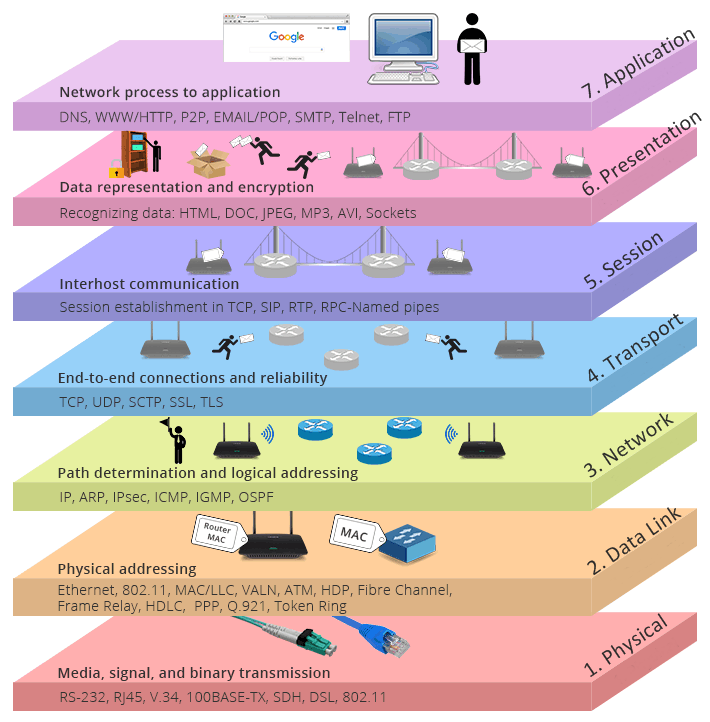
\includegraphics[width=0.70\textwidth,height=0.50\textheight,keepaspectratio]{image4.png}
\fonte{Adaptado de \citeonline{tanenbaum2021redes} e \citeonline{forouzan2010comunicacao}.}
\end{figure}

Na prática, a Internet consolidou-se sobre a arquitetura TCP/IP (RFC 1180), estruturada em quatro camadas operacionais \cite{sipple1991tcpip}. Na camada de aplicação, operam protocolos como HTTP/HTTPS e DNS, além do SNMP para gerenciamento. Na camada de transporte, o TCP provê entrega orientada a conexão e confiável, enquanto o UDP prioriza velocidade e baixo \textit{overhead}, sendo o transporte padrão das consultas SNMP. Na camada de rede, o protocolo ICMP viabiliza diagnósticos essenciais como o teste de conectividade \textit{Ping} \cite{forouzan2010comunicacao}, estruturado em camadas como exibido na Figura \ref{fig:modelo_tcp_ip}.

\begin{figure}[H]
\centering
\caption{Camadas do modelo TCP/IP}
\label{fig:modelo_tcp_ip}
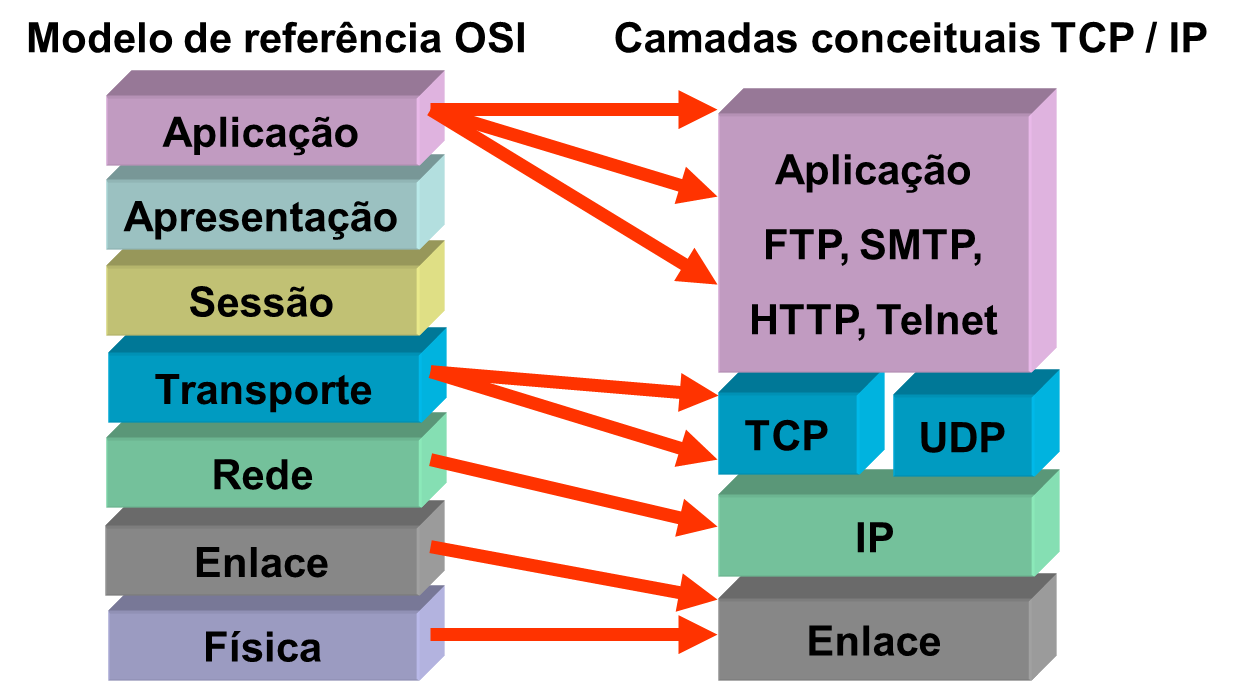
\includegraphics[width=0.85\textwidth,height=0.50\textheight,keepaspectratio]{image5.png}
\fonte{Adaptado de \citeonline{kurose2013redes} e \citeonline{sipple1991tcpip}.}
\end{figure}

\subsection{GERENCIAMENTO DE REDES E PROTOCOLO SNMP}
O modelo FCAPS (\textit{Fault, Configuration, Accounting, Performance, Security}), definido pela ISO, categoriza a administração de redes em cinco áreas funcionais. O NetSpot concentra sua atuação no Gerenciamento de Desempenho (\textit{Performance Management}) e no Gerenciamento de Falhas (\textit{Fault Management}), visando identificar e mitigar anomalias operacionais de maneira preditiva \cite{tanenbaum2021redes}.

O protocolo SNMP (\textit{Simple Network Management Protocol}), formalizado inicialmente pela IETF na RFC 1157 \cite{case1990rfc1157} e estruturado arquiteturalmente na RFC 3411 \cite{harrington2002rfc3411}, é o padrão da indústria para monitoramento de ativos. Trabalhando na camada de aplicação e apropriando-se primariamente da leveza do UDP, o protocolo opera de forma centralizada através de três grandes componentes: Gerente (estação de monitoramento), pelos Agentes (softwares/daemons que rodam nos equipamentos monitorados) e as MIBs (\textit{Management Information Bases}). A MIB atua como um banco de dados virtual hierárquico, organizado por identificadores de objeto OIDs (\textit{Object Identifiers}), cujo papel é armazenar de maneira sistemática todas as variáveis, métricas e estatísticas relativas ao estado do dispositivo.
A flexibilidade do SNMP advém da sua simplicidade operacional baseada em PDUs (\textit{Protocol Data Units}) como \texttt{GetRequest} (para solicitar a leitura do valor de uma variável), \texttt{SetRequest} (para alterar ou configurar um parâmetro remotamente) e \texttt{Trap} (uma notificação assíncrona, não solicitada pelo gerente, em que o agente envia o alerta sobre um evento excepcional ou falha iminente), conforme sintetizado na Figura \ref{fig:arquitetura_snmp}.

\begin{figure}[H]
\centering
\caption{Arquitetura SNMP}
\label{fig:arquitetura_snmp}
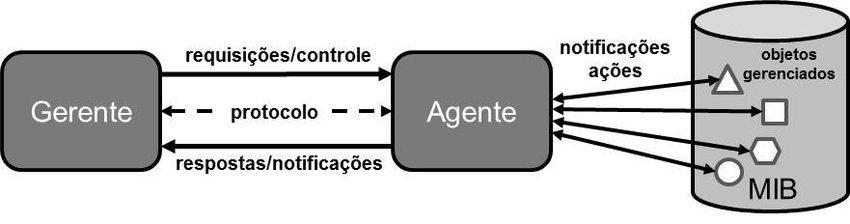
\includegraphics[width=0.82\textwidth]{image1.jpg}
\fonte{Adaptado de \citeonline{basso2020administracao} e \citeonline{harrington2002rfc3411}.}
\end{figure}

Enquanto as versões SNMPv1 e v2c baseiam sua segurança na troca de strings de comunidade em texto claro (\textit{plaintext}), vulneráveis a ataques de interceptação (\textit{sniffing}), a versão SNMPv3 introduz o modelo USM (\textit{User-based Security Model}), provendo autenticação criptográfica (MD5/SHA) e privacidade dos dados via encriptação (DES/AES), garantindo a conformidade com requisitos modernos de segurança da informação.

\subsection{TRABALHOS CORRELATOS}
Inúmeros trabalhos científicos e técnicos vêm explorando metodologias de monitoramento ativo para prevenir degradações. \citeonline{zarpelao2010deteccao}, por exemplo, utilizou um nível avançado de modelagem do tráfego para detectar anomalias, correlacionando múltiplos alarmes através de grafos de dependência entre objetos SNMP para conferir uma visão panorâmica do problema ao administrador. \citeonline{faccine2019aplicacao}, por sua vez, desenvolveu uma aplicação web baseada em SNMP e RRDtool capaz de coletar métricas de tráfego de interfaces de rede, como taxas de entrada e saída de bytes e descarte de pacotes, exibindo-as em gráficos atualizados em tempo real para auxiliar o administrador na tomada de decisões. \citeonline{rodrigues2025monitoramento} e a \citeonline{utfpr2016implementacao} analisaram a aplicação do Zabbix em infraestruturas acadêmicas, ressaltando sua ampla capacidade de telemetria e maturidade, mas evidenciando a elevada complexidade de parametrização de templates e o esforço de configuração inicial exigido das equipes técnicas. \citeonline{hentges2022monitoramento} comprovaram na prática como a automatização do SNMP agilizou drasticamente a resolução de chamados de suporte na rede pública de Arroio do Meio.

A relevância do monitoramento específico é corroborada por \citeonline{silva2024prototipo}, que validou a criação de um protótipo de detecção de oscilações de sinal focado estritamente na realidade de provedores (ISPs) de pequeno porte. Dentro da área de soluções leves (\textit{lightweight}), destacam-se a proposta de \citeonline{yahya2017lightweight} que, frente às fortes limitações da Internet das Coisas (IoT), conseguiram diminuir pacotes SNMP em 40\% reduzindo também a exigência de CPU dos dispositivos restritos, e o estudo de \citeonline{roquero2021performance} com a formulação de algoritmos inteligentes de \textit{polling} visando escalabilidade eficiente para grandes datacenters sem elevação extrema de custos computacionais. Na busca por mitigação de latência durante o processamento corporativo, \citeonline{espinel2022design} obtiveram sucesso distribuindo as atividades do SNMP através de um modelo multi-agente operado em camadas (coletor, consolidador e aplicação). Para o monitoramento com alertas, os frameworks analisados por \citeonline{khan2013efficient}, \citeonline{liu2012monitoring} e \citeonline{liu2013design} reforçam a eficácia de correlacionar métricas SNMP contínuas com alertas disparados instantaneamente após falhas na rede.

Contudo, ao analisar profundamente a literatura supracitada, constata-se uma lacuna nítida frente à demanda de estruturas de pequeno e médio portes, nas quais implantar e manter plataformas corporativas tradicionais torna-se contraproducente devido à complexidade de instalação inicial, necessidade de administração de múltiplos componentes auxiliares, curva de aprendizado íngreme e esforço contínuo de manutenção de templates e exporters. O diferencial inerente do NetSpot reside precisamente na concepção de uma ferramenta no conceito NOC Lite: focada na extrema praticidade operacional, facilidade de uso com interface intuitiva, baixo consumo computacional e implantação descomplicada via contêineres prontos para uso (\textit{turn-key}), sustentada por uma Arquitetura Orientada a Eventos (EDA) assíncrona em Python (3.11/3.12) com resiliência auto-regenerativa (\textit{Circuit Breaker}, \textit{Self-Healing}, DLQ e \textit{Anti-Spam}) e automação de alertas preventivos.

\section{METODOLOGIA}
Esta seção descreve os procedimentos metodológicos, o método de engenharia de software e a estratégia experimental adotados no desenvolvimento e na avaliação empírica do NetSpot.

\subsection{CLASSIFICAÇÃO DA PESQUISA}
Quanto à sua finalidade, esta pesquisa classifica-se como \textbf{aplicada}, uma vez que objetiva conceber, implementar e validar uma solução tecnológica funcional para um problema prático concreto vivenciado na administração de infraestruturas de TIC: o monitoramento proativo, leve e de alta disponibilidade em redes de pequeno e médio porte e laboratórios de ensino.

Quanto à abordagem do problema, o trabalho adota natureza \textbf{quali-quantitativa (mista)}. A vertente qualitativa manifesta-se na modelagem arquitetural orientada a objetos, na análise ergonômica da experiência do operador NOC e na inferência heurística de causa raiz para incidentes operacionais. A vertente quantitativa evidencia-se na mensuração empírica e contínua de variáveis de telemetria de rede (RTT, \textit{jitter}, vazão de tráfego, percentual de SLA e \textit{Health Score}), bem como na aferição do consumo de recursos computacionais (taxa de ocupação de CPU e alocação de memória RAM) sob regimes controlados de estresse.

No que tange aos seus objetivos operacionais, a pesquisa caracteriza-se como \textbf{descritivo-exploratória}, detalhando os comportamentos de resiliência e os impactos de anomalias induzidas em ativos físicos e virtuais. Sob o prisma dos procedimentos técnicos, o estudo ancora-se no método experimental fundamentado no paradigma de \textit{Design Science Research} (DSR) e na Engenharia de Software, cujo ciclo metodológico compreende a identificação do problema, a especificação de requisitos, a síntese do artefato computacional e sua rigorosa validação em ambientes simulados e reais.

\subsection{MÉTODO DE ENGENHARIA E MODELAGEM DE SOFTWARE}
O desenvolvimento do NetSpot orientou-se pelo método de Análise e Projeto de Sistemas de Informação Orientados a Objetos formalizado por \citeonline{wazlawick2011analise}, articulado às boas práticas contemporâneas de Engenharia de Software \cite{engsoftmoderna} e aos preceitos da Arquitetura Limpa \cite{martin2019arquitetura}.

A elicitação e a estruturação dos contratos operacionais do sistema basearam-se no modelo conceitual FURPS+:
\begin{itemize}[leftmargin=1.25cm]
\item \textbf{Funcionalidade (\textit{Functionality})}: Descoberta automática de nós em sub-redes IPv4 locais (\textit{LAN Discovery}), sondagens ativas multicamada concorrentes (ICMP \textit{Ping}, verificação de portas de transporte TCP, requisições L7 HTTP/HTTPS com inspeção de cabeçalhos) e telemetria profunda de hardware via protocolo SNMP (UCD-SNMP-MIB e HOST-RESOURCES-MIB);
\item \textbf{Usabilidade (\textit{Usability})}: Interface web em arquitetura SPA (\textit{Single Page Application}) com cartões tridimensionais de telemetria, modo alternativo de Tabela NOC para visualização massiva de densidade, transição suave de temas visual (\textit{Dark and White}) e conformidade estrita com as diretrizes de acessibilidade W3C WCAG 2.1 nível AA \cite{w3c2018wcag21};
\item \textbf{Confiabilidade e Resiliência (\textit{Reliability})}: Tolerância a falhas via barramento desacoplado RabbitMQ com \textit{Dead Letter Queue} (DLQ), disjuntor de proteção (\textit{Circuit Breaker}) para prevenção de falhas em cascata \cite{nygard2018release}, algoritmo heurístico de supressão compensatória para firewalls de inspeção de estado e filtro anti-flapping composto para contenção de tempestades de alertas;
\item \textbf{Desempenho (\textit{Performance})}: Motor de I/O assíncrono em Python (3.11/3.12) suportado por \texttt{asyncio}, garantindo ciclos completos de varredura sobre dezenas de nós em janela inferior a 2 segundos, mantendo consumo estável abaixo de 600 MB de RAM e teto de CPU sob 12\%;
\item \textbf{Suportabilidade (\textit{Supportability})}: Modularização em cinco microsserviços containerizados via Docker, permitindo implantação imediata (\textit{turn-key}) e reprodutível sem dependência de configurações prévias complexas no sistema operacional hospedeiro.
\end{itemize}

A atribuição de responsabilidades operacionais nas camadas de domínio e de serviço seguiu os padrões GRASP formalizados por \citeonline{larman2005utilizando}, priorizando alta coesão e baixo acoplamento.

\subsection{ESTRATÉGIA HÍBRIDA DE EXPERIMENTAÇÃO E CONTROLE}
Para assegurar a validade experimental dos resultados sem interferir na operação pedagógica dos laboratórios institucionais, concebeu-se uma estratégia de validação híbrida, combinando a emulação virtualizada em larga escala com a experimentação física controlada.

As estações de trabalho e servidores dos laboratórios de informática do IFNMG -- Campus Januária possuem grade horária contínua e prioritária dedicada às aulas pedagógicas dos cursos técnicos e superiores. Consequentemente, intervenções destrutivas prolongadas — tais como saturação massiva de enlaces, alteração de parâmetros de kernel de roteamento, desativação forçada de regras de firewall e injeção de sobrecarga de hardware — revelaram-se inviáveis para evitar qualquer prejuízo às atividades letivas.

Frente a essa contingência real, a metodologia estruturou-se em duas frentes empíricas:
\begin{enumerate}[leftmargin=1.25cm]
\item \textbf{Emulação Virtualizada em Larga Escala com o Framework Kathar{\'a} \cite{bonola2018kathara}}:
Permitiu submeter o NetSpot a condições extremas de rede através de dois laboratórios reprodutíveis: a topologia canônica de 40 nós monitorados distribuídos em três domínios de broadcast com roteadores Quagga/FRRouting intermediários, e o cenário de estresse em alta densidade com 126 nós monitorados simultaneamente sob o bloco de endereçamento \texttt{10.0.0.0/22}. Nesse ambiente, foram injetadas anomalias intencionais e controladas utilizando utilitários de perturbação de tráfego (\texttt{tc} para injeção de atraso e descarte aleatório de pacotes) e sobrecarga computacional (\texttt{stress-ng});
\item \textbf{Validação Física em Ambiente Real (Laboratório 2 do IFNMG -- Campus Januária)}:
Conduzida durante as janelas de disponibilidade programada dos laboratórios de ensino, a experimentação física abrangeu estações de trabalho reais interconectadas à rede local acadêmica sob ecossistemas heterogêneos (Ubuntu Linux e Windows 10/11 Pro). O sistema foi avaliado quanto à sua capacidade de descobrir os ativos automaticamente através de varredura de sub-rede, resolver OIDs SNMP polimórficos de hardware em tempo real e notificar anomalias decorrentes da desconexão física deliberada de cabos de rede e derrubada de serviços locais.
\end{enumerate}

\subsection{INSTRUMENTOS DE COLETA, TELEMETRIA E CRITÉRIOS DE VALIDAÇÃO}
Os dados empíricos foram coletados e armazenados continuamente através dos seguintes mecanismos:
\begin{itemize}[leftmargin=1.25cm]
\item \textbf{Telemetria de Rede e Protocolos}: Amostragem contínua de tempos de resposta RTT (ICMP e TCP) e L7 (HTTP), sintetizados estatisticamente através do cálculo de \textit{Jitter} conforme a RFC 3550 \cite{schulzrinne2003rfc3550}, mensuração de conformidade de SLA via união de intervalos contíguos de tempo (\textit{Interval Merging}) baseada no problema da medida de Klee \cite{bentley1977klee} e estimativa de tendência preditiva por Mínimos Quadrados Ordinários (OLS);
\item \textbf{Telemetria de Consumo Computacional}: Monitoramento dos recursos alocados pelo servidor de gerência através das ferramentas nativas \texttt{docker stats} e \texttt{htop}, registrando o percentual de ocupação de CPU, o consumo absoluto de memória RAM e a taxa de I/O em disco ao longo de execuções prolongadas;
\item \textbf{Verificação Formal de Regras de Negócio e Segurança}: Auditoria exaustiva da suíte de 86 testes automatizados desenvolvida em Pytest (\texttt{Backend/tests/}), contemplando a validação de algoritmos analíticos, o ciclo de estados do disjuntor de resiliência e a proteção contra regressões críticas de segurança (RLS, RBAC, criptografia de credenciais via Bcrypt \cite{provos1999bcrypt} e blindagem contra injeção de scripts maliciosos XSS).
\end{itemize}

\section{ARQUITETURA E IMPLEMENTAÇÃO DO NETSPOT}
O \textbf{NetSpot (NOC Lite)} foi concebido e implementado sob os preceitos fundamentais da Análise e Projeto de Sistemas Orientados a Objetos formalizados por \citeonline{wazlawick2011analise}, articulados aos princípios da \textit{Clean Architecture} \cite{engsoftmoderna}, aos padrões SOLID e à orquestração de microsserviços containerizados orientados a eventos. O sistema estabelece uma abordagem estritamente desacoplada na qual as regras de negócio centrais independem de bibliotecas externas, frameworks de apresentação ou especificidades de bancos de dados.

A solução é isolada em 5 microsserviços interdependentes executados via Docker e gerenciados através de uma rede interna em ponte (\textit{bridge network}), conforme ilustrado na Figura \ref{fig:arquitetura_eda}:
\begin{enumerate}[leftmargin=1.25cm]
\item \textbf{Backend FastAPI (Python 3.11/3.12)}: Núcleo computacional do sistema, responsável pelo agendador assíncrono de checagens (\textit{Scheduler}), rotinas de ingestão via APIs RESTful, algoritmos matemáticos de telemetria NOC, gerenciamento do disjuntor (\textit{Circuit Breaker}) e motor de coleta SNMP multivendor.
\item \textbf{PostgreSQL 15}: Sistema gerenciador de banco de dados relacional (SGBD) responsável pela persistência das configurações dos ativos, séries temporais de telemetria, registros de incidentes e trilhas de auditoria, operando com pool de conexões auto-regenerativo via SQLAlchemy e AsyncPG, com suporte nativo a políticas de segurança em nível de linha (\textit{Row Level Security} -- RLS).
\item \textbf{RabbitMQ 3}: Barramento de mensageria assíncrona baseado no protocolo AMQP (\textit{Advanced Message Queuing Protocol}), encarregado de desacoplar o motor de coleta do processamento de notificações e fornecer garantia de entrega através de filas dedicadas e tolerância a falhas via \textit{Dead Letter Queue} (DLQ).
\item \textbf{N8N Automation Engine}: Orquestrador programável de fluxos de trabalho que consome eventos publicados no barramento AMQP, executando transformações de dados, controle de janelas de agregação e despacho de notificações para a API do Telegram com templates HTML sanitizados contra injeção de código.
\item \textbf{Nginx Alpine (Frontend SPA)}: Servidor web leve e de alta performance, configurado para servir a interface do usuário estática (\textit{Single Page Application}) em HTML5, CSS e JavaScript puros (100\% \textit{offline-first} com fontes WOFF2 locais), atuando simultaneamente como proxy reverso de baixa latência para os endpoints da API REST do backend.
\end{enumerate}

\begin{figure}[H]
\centering
\caption{Arquitetura Orientada a Eventos do NetSpot}
\label{fig:arquitetura_eda}
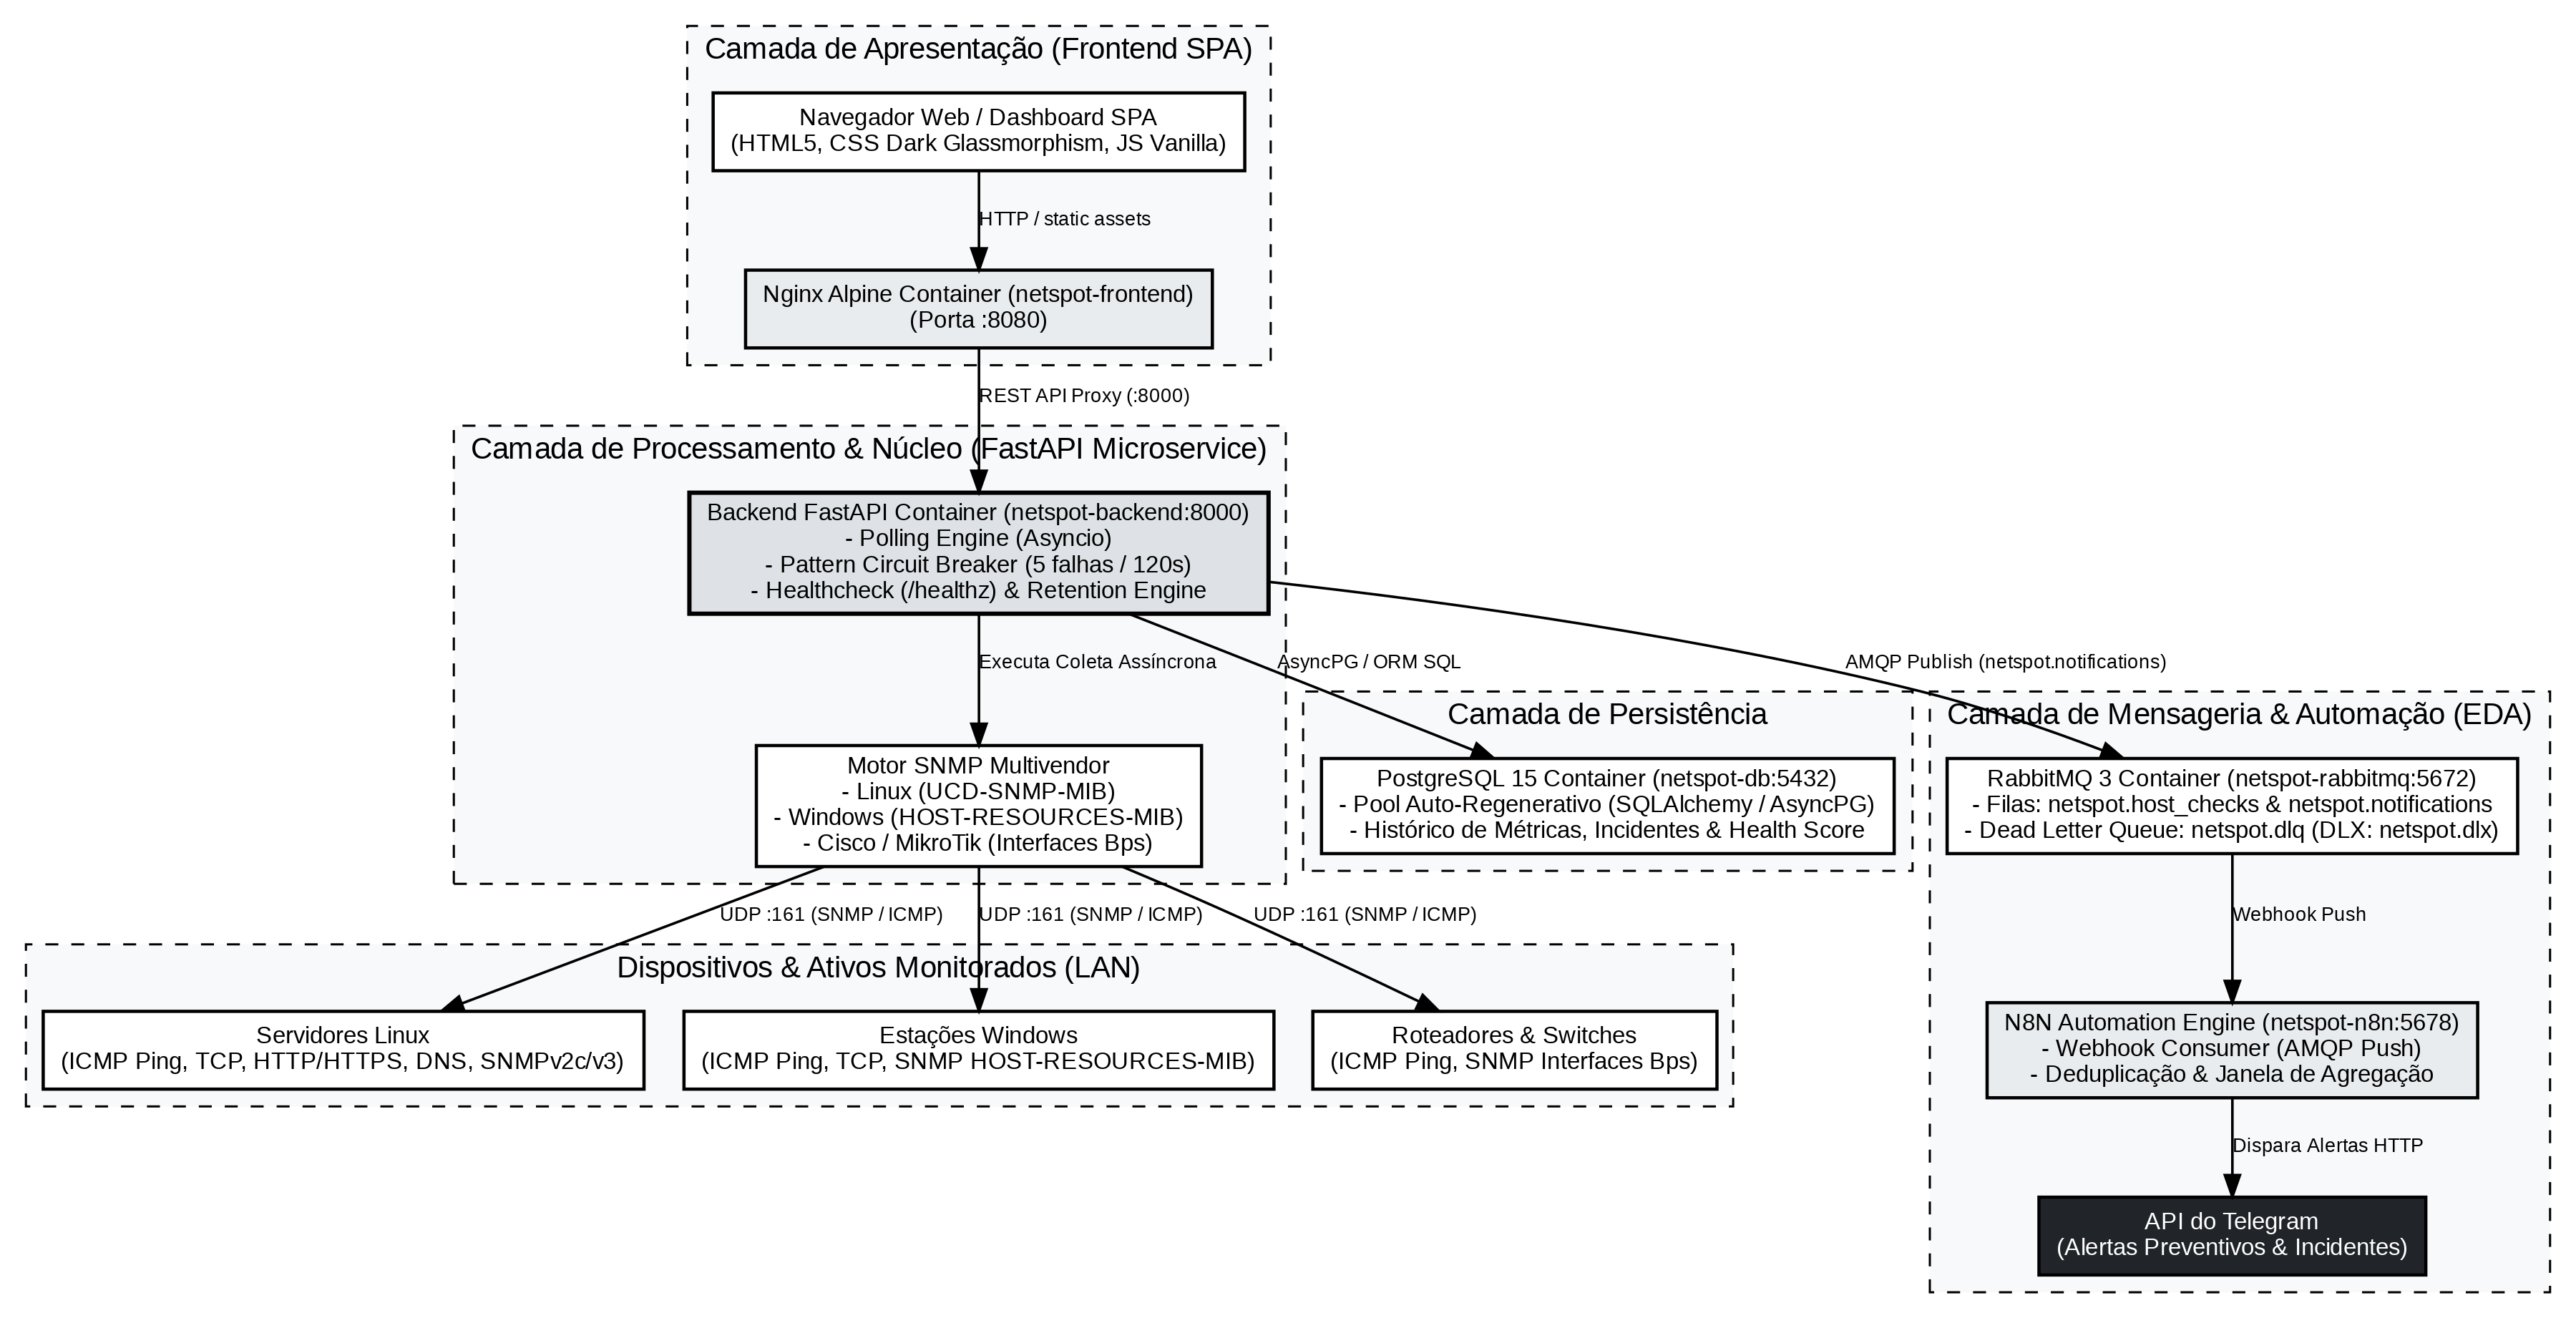
\includegraphics[width=0.94\textwidth]{image3.png}
\fonte{Autoria própria (2026).}
\end{figure}

\subsection{MODELAGEM DE DADOS E DIAGRAMA DE CLASSES DO PROJETO}
A estrutura orientada a objetos do NetSpot foi concebida sob os preceitos de baixo acoplamento e alta coesão, refletindo a separação formal entre entidades de domínio persistidas em banco relacional, classes de serviço assíncronas responsáveis pela orquestração de resiliência e contratos de dados (\textit{Data Transfer Objects} -- DTOs) validados pelo Pydantic. A persistência dos dados é mediada pelo SQLAlchemy ORM sobre o PostgreSQL 15, garantindo integridade referencial, indexação otimizada para séries temporais e suporte nativo a exclusão lógica (\textit{Soft Delete}).

A Figura \ref{fig:diagrama_classes} ilustra a modelagem arquitetural completa do NetSpot, organizada em três pacotes conceituais complementares:

\begin{figure}[H]
\centering
\caption{Diagrama de classes UML expandido e modelagem arquitetural do NetSpot}
\label{fig:diagrama_classes}
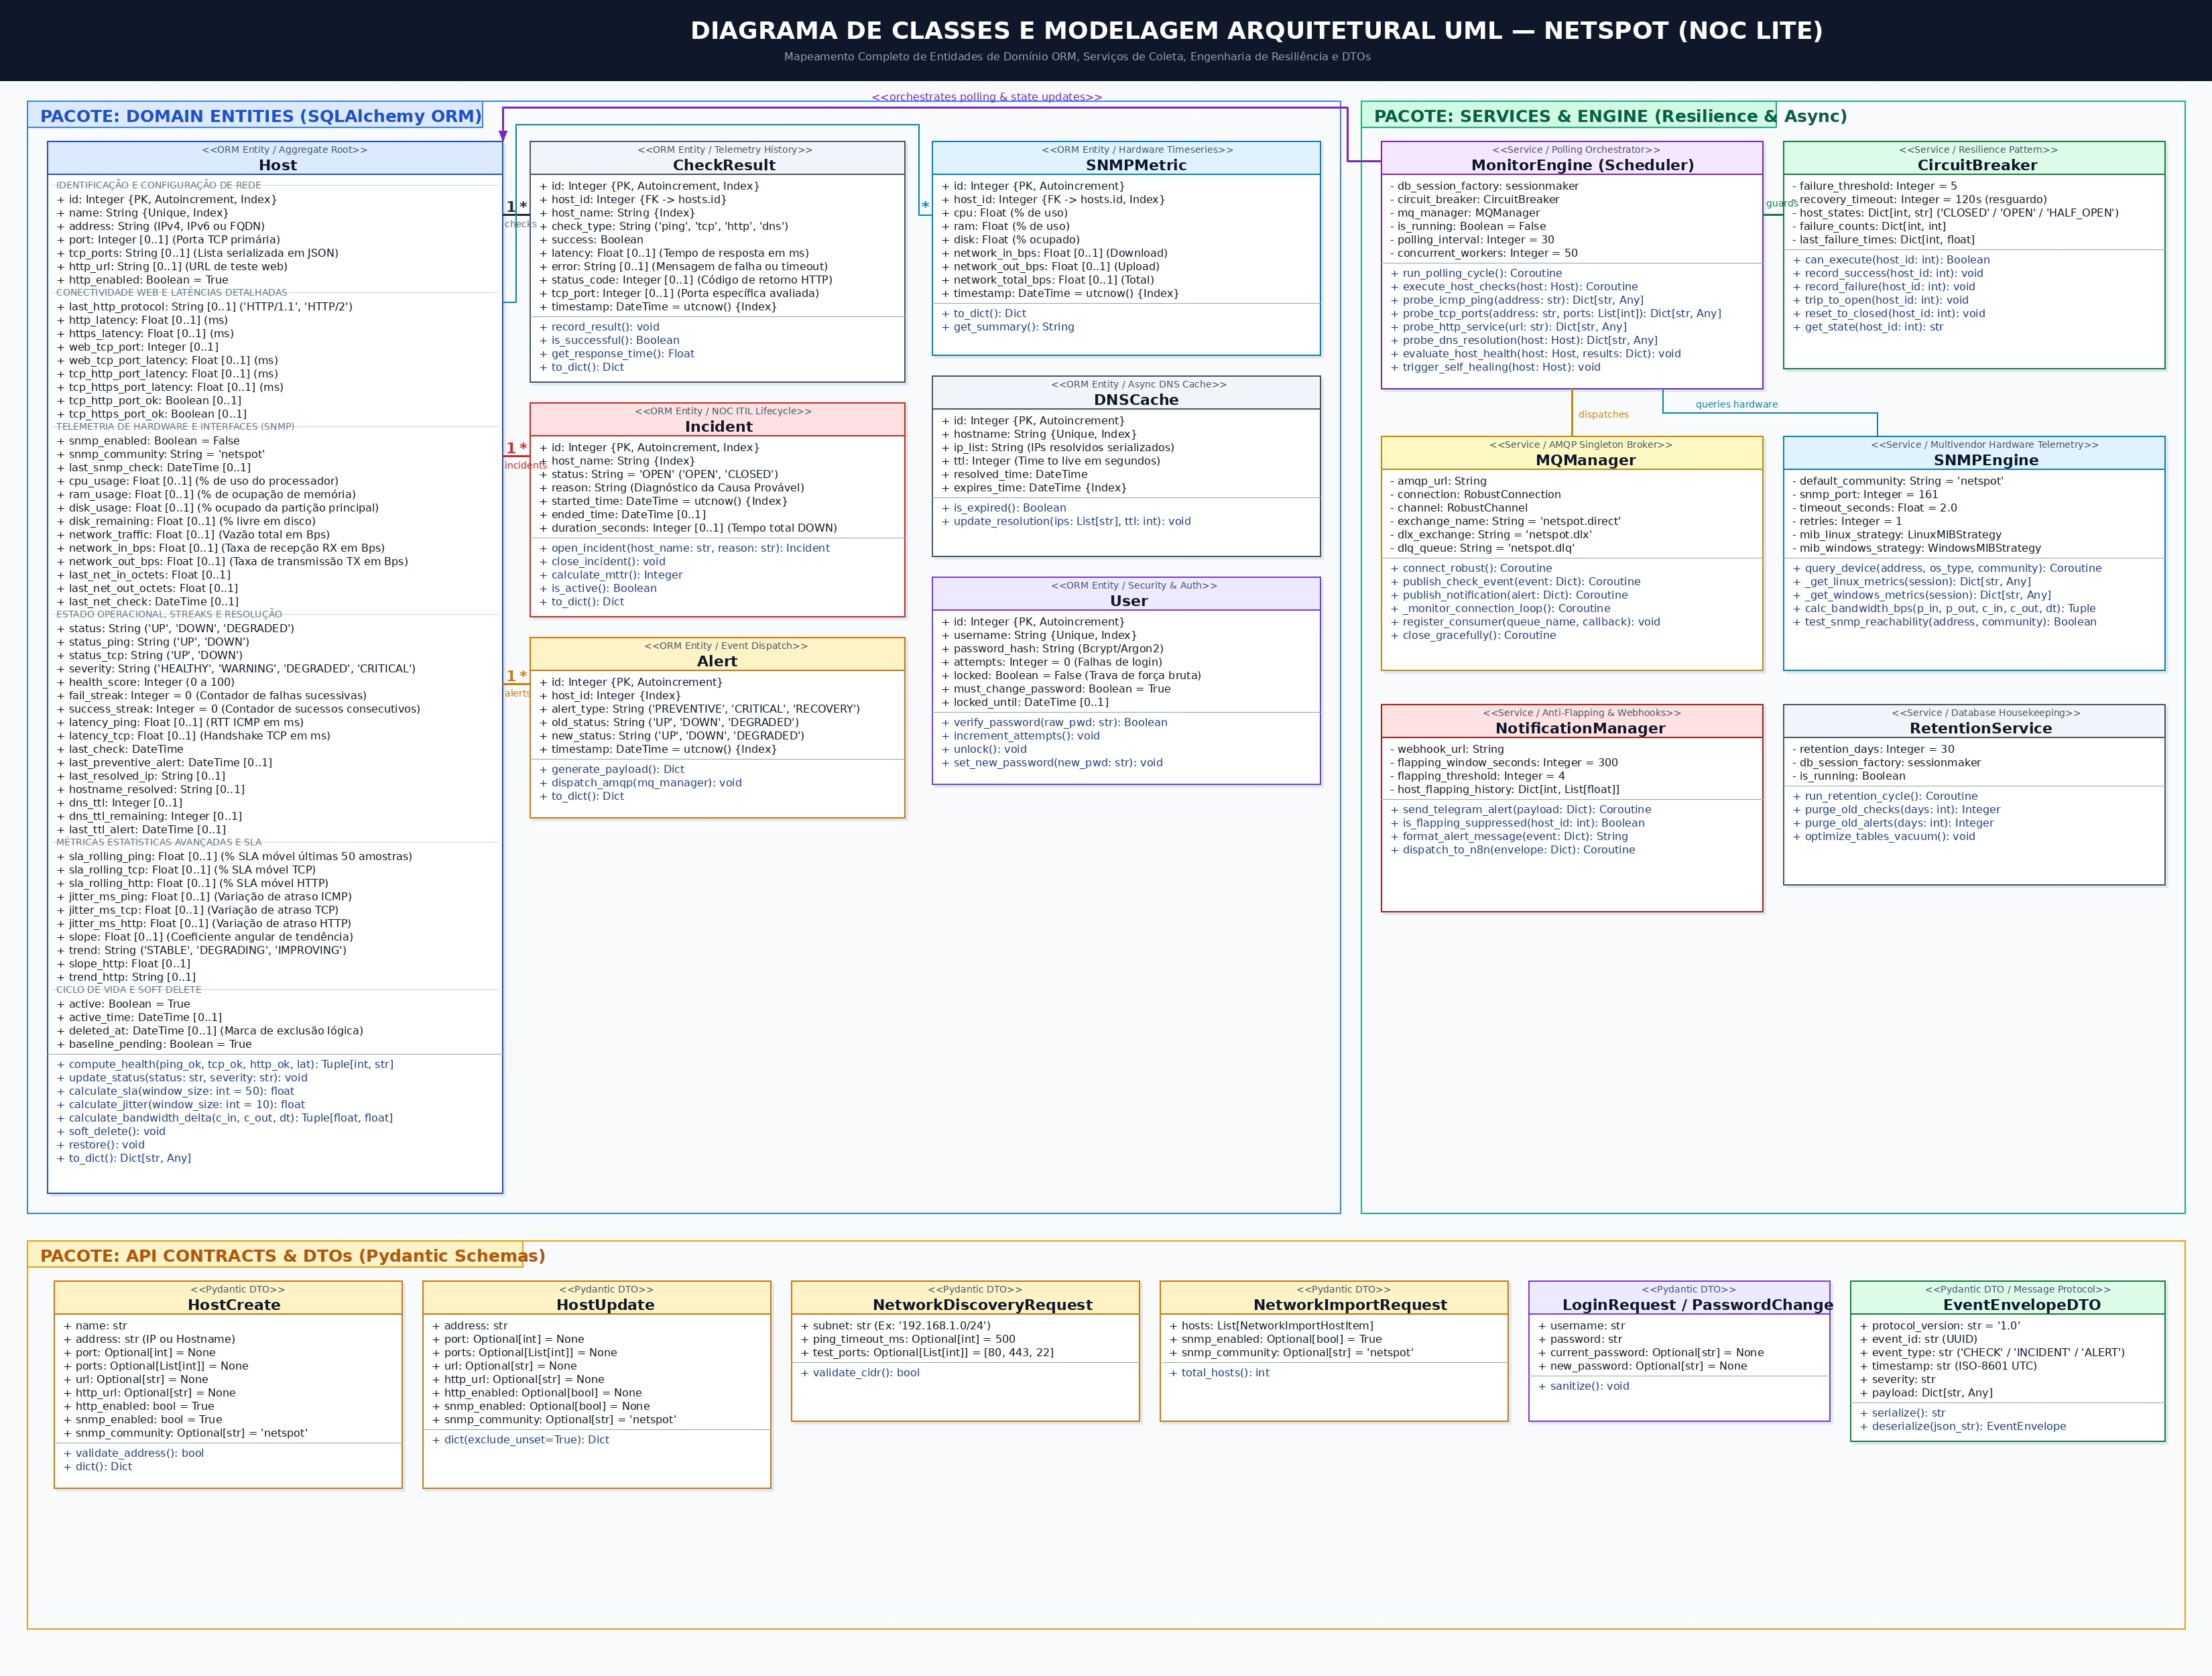
\includegraphics[width=0.98\textwidth]{diagrama_classes.jpg}
\fonte{Autoria própria (2026).}
\end{figure}

Conforme detalhado no modelo da Figura \ref{fig:diagrama_classes}, a arquitetura estrutura-se em:
\begin{enumerate}[leftmargin=1.25cm]
\item \textbf{Pacote 1: Entidades de Domínio e Persistência (SQLAlchemy ORM)}: Abrange as tabelas relacionais do sistema. A classe \texttt{Host} atua como o agregado nuclear (\textit{Aggregate Root}), centralizando as configurações cadastrais e métricas consolidadas, estabelecendo relações $1 \to *$ com as checagens históricas (\texttt{CheckResult}), incidentes operacionais (\texttt{Incident}), alarmes despachados (\texttt{Alert}) e séries temporais de hardware (\texttt{SNMPMetric}). Complementam o domínio a tabela de cache DNS assíncrono (\texttt{DNSCache}) e o controle de segurança (\texttt{User});
\item \textbf{Pacote 2: Serviços de Coleta, Resiliência e Infraestrutura}: Encapsula a inteligência assíncrona do sistema, incluindo o disjuntor de sobrecarga (\texttt{CircuitBreaker}), o conector resiliente de mensageria (\texttt{MQManager}), o orquestrador concorrente (\texttt{MonitorEngine}), o módulo de telemetria heterogênea (\texttt{SNMPEngine}), a supressão de fadiga de alarmes (\texttt{NotificationManager}) e o expurgo automático (\texttt{RetentionService});
\item \textbf{Pacote 3: Contratos da API e DTOs (Pydantic Schemas)}: Formaliza a validação estrita de entradas e saídas HTTP, garantindo segurança de tipos na criação de hosts (\texttt{HostCreate}), atualizações parciais (\texttt{HostUpdate}), varreduras de sub-rede (\texttt{NetworkDiscoveryRequest}), importações em lote (\texttt{NetworkImportRequest}) e no envelope de mensagens (\texttt{EventEnvelopeDTO}).
\end{enumerate}

\subsubsection{Entidades de Domínio e Modelo Relacional}
O núcleo de persistência organiza-se em torno de 7 entidades principais (\texttt{Backend/models.py}), cujo detalhamento técnico é apresentado a seguir:

\begin{itemize}[leftmargin=1.25cm]
\item \textbf{Host (\texttt{hosts})}: Entidade central e mais abrangente do sistema, agregando quase 50 colunas estruturadas em cinco blocos operacionais:
  \begin{itemize}
  \item \textit{Identificação e Configuração de Rede}: \texttt{id} (chave primária indexada), \texttt{name} (rótulo identificador exclusivo), \texttt{address} (endereço IPv4, IPv6 ou FQDN), \texttt{port} (porta TCP padrão), \texttt{tcp\_ports} (vetor de portas monitoradas serializado em JSON), \texttt{http\_url} (URL web opcional) e flags booleanas \texttt{http\_enabled} e \texttt{snmp\_enabled};
  \item \textit{Conectividade Web e Latências Detalhadas}: \texttt{last\_http\_protocol} (protocolo negociado, ex.: HTTP/1.1 ou HTTP/2), \texttt{http\_latency} e \texttt{https\_latency} em milissegundos, \texttt{web\_tcp\_port}, \texttt{web\_tcp\_port\_latency}, \texttt{tcp\_http\_port\_latency}, \texttt{tcp\_https\_port\_latency} e os booleanos de conformidade \texttt{tcp\_http\_port\_ok} e \texttt{tcp\_https\_port\_ok};
  \item \textit{Telemetria de Hardware SNMP}: \texttt{snmp\_community} (comunidade de acesso, padrão \texttt{``netspot''}), \texttt{last\_snmp\_check}, consumo percentual instantâneo de processador (\texttt{cpu\_usage}), memória RAM (\texttt{ram\_usage}) e disco principal (\texttt{disk\_usage}), folga de armazenamento (\texttt{disk\_remaining}), vazão agregada (\texttt{network\_traffic}) e taxas unidirecionais de entrada (\texttt{network\_in\_bps}) e saída (\texttt{network\_out\_bps}), além dos contadores brutos de octetos acumulados (\texttt{last\_net\_in\_octets} e \texttt{last\_net\_out\_octets}) e marcação temporal (\texttt{last\_net\_check});
  \item \textit{Estado Operacional, Contadores e Resolução}: \texttt{status} ($\in \{\text{UP, DOWN, DEGRADED}\}$), granularidades \texttt{status\_ping} e \texttt{status\_tcp}, classificação de urgência (\texttt{severity} $\in \{\text{HEALTHY, WARNING, DEGRADED, CRITICAL}\}$), índice sintético \texttt{health\_score} (0 a 100\%), contadores de persistência de falhas (\texttt{fail\_streak}) e sucessos consecutivos (\texttt{success\_streak}), latências pontuais (\texttt{latency\_ping}, \texttt{latency\_tcp}), carimbos temporais (\texttt{last\_check}, \texttt{last\_preventive\_alert}), mapeamento DNS resolvido (\texttt{last\_resolved\_ip}, \texttt{hostname\_resolved}) e auditoria de TTL (\texttt{dns\_ttl}, \texttt{dns\_ttl\_remaining}, \texttt{last\_ttl\_alert});
  \item \textit{Métricas Estatísticas e Ciclo de Vida}: SLA móvel das últimas 50 amostras (\texttt{sla\_rolling\_ping}, \texttt{sla\_rolling\_tcp}, \texttt{sla\_rolling\_http}), variação de latência em milissegundos (\texttt{jitter\_ms\_ping}, \texttt{jitter\_ms\_tcp}, \texttt{jitter\_ms\_http}), coeficiente angular de regressão (\texttt{slope}, \texttt{slope\_http}), tendência qualitativa (\texttt{trend} e \texttt{trend\_http} $\in \{\text{STABLE, DEGRADING, IMPROVING}\}$), controle de exclusão lógica (\texttt{deleted\_at}, permitindo recuperação na lixeira) e estado de aferição de linha de base (\texttt{baseline\_pending}).
  \item \textit{Desacoplamento e Métodos}: Sob as diretrizes de \textit{Clean Architecture}, os algoritmos estatísticos de cálculo de disponibilidade (\texttt{calculate\_sla()}), oscilação de latência (\texttt{calculate\_jitter()}), vazão de banda (\texttt{calculate\_bandwidth\_delta()}) e consolidação sintética (\texttt{compute\_health\_score()}) foram desacoplados do modelo ORM, residindo como serviços analíticos puros no módulo \texttt{Backend/metrics.py}. A entidade \texttt{Host} preserva o estado relacional e o ciclo de vida de persistência (\textit{soft delete} e restauração via carimbo em \texttt{deleted\_at}).
  \end{itemize}
\item \textbf{CheckResult (\texttt{checks})}: Armazena cada amostragem individual realizada pelos checadores multi-protocolo, viabilizando análises históricas e auditoria. Contém chave estrangeira para o host (\texttt{host\_id}), \texttt{check\_type} (ping, tcp, http ou dns), booleano de sucesso (\texttt{success}), tempo de resposta em milissegundos (\texttt{latency}), mensagem de erro (\texttt{error}), código de status HTTP (\texttt{status\_code}), porta TCP avaliada (\texttt{tcp\_port}) e carimbo temporal UTC (\texttt{timestamp}).
\item \textbf{Incident (\texttt{incidents})}: Gerencia o ciclo de vida dos incidentes operacionais da infraestrutura. Registra o ativo impactado (\texttt{host\_name}), status operacional (\texttt{status} $\in \{\text{OPEN, CLOSED}\}$), diagnóstico causal (\texttt{reason}), instante de abertura da indisponibilidade (\texttt{started\_time}), momento do restabelecimento (\texttt{ended\_time}) e a duração total em segundos (\texttt{duration\_seconds}), viabilizando o cálculo do tempo médio de reparo (\textit{Mean Time to Repair} -- MTTR).
\item \textbf{Alert (\texttt{alerts})}: Rastreia os eventos de alerta preventivos e corretivos, registrando o host associado (\texttt{host\_id}), tipo de alarme (\texttt{alert\_type}), transição de estado (\texttt{old\_status} para \texttt{new\_status}) e registro temporal (\texttt{timestamp}).
\item \textbf{DNSCache (\texttt{dns\_cache})}: Provê resolução local de nomes para mitigar requisições repetitivas a servidores DNS raiz, controlando mapeamentos (\texttt{hostname}, \texttt{ip\_list}), tempo de vida nominal (\texttt{ttl}), instante da resolução (\texttt{resolved\_time}) e tempo de expiração (\texttt{expires\_time}).
\item \textbf{User (\texttt{users})}: Suporta o módulo de autenticação e segurança, contendo \texttt{username}, \texttt{password\_hash} (criptografia com algoritmo Bcrypt \cite{provos1999bcrypt} com derivação de chaves e salt individualizado), contador de tentativas falhas de login (\texttt{attempts}), bloqueio por força bruta (\texttt{locked}, \texttt{locked\_until}) e sinalizador de troca obrigatória de credenciais no primeiro acesso (\texttt{must\_change\_password}).
\item \textbf{SNMPMetric (\texttt{snmp\_metrics})}: Tabela dedicada ao armazenamento de séries temporais granulares de hardware (\texttt{host\_id}, \texttt{cpu}, \texttt{ram}, \texttt{disk}, \texttt{network\_in\_bps}, \texttt{network\_out\_bps}, \texttt{network\_total\_bps}, \texttt{timestamp}), alimentando os gráficos de tendências do painel.
\end{itemize}

A Tabela \ref{tab:entidades_relacionais} sintetiza o mapeamento estrutural das entidades de domínio, suas chaves e responsabilidades no NetSpot:

\begin{table}[H]
\centering
\caption{Mapeamento das entidades relacionais e atributos do NetSpot}
\label{tab:entidades_relacionais}
\small
\begin{tabular}{@{}p{2.8cm}p{3.2cm}p{3.0cm}p{6.0cm}@{}}
\toprule
\textbf{Entidade / Tabela} & \textbf{Chave Primária / FK} & \textbf{Principais Atributos} & \textbf{Papel no Sistema} \\
\midrule
\texttt{Host} (\texttt{hosts}) & \texttt{id} (PK) & \texttt{name, address, status, health\_score, deleted\_at} & Registro mestre do ativo, telemetria consolidada e suporte a \textit{soft delete}. \\
\texttt{CheckResult} (\texttt{checks}) & \texttt{id} (PK) / \texttt{host\_id} (FK) & \texttt{check\_type, success, latency, status\_code} & Amostras pontuais de telemetria para cálculo de SLA e Jitter. \\
\texttt{Incident} (\texttt{incidents}) & \texttt{id} (PK) & \texttt{host\_name, status, started\_time, duration} & Rastreabilidade de falhas e mensuração contínua de MTTR. \\
\texttt{Alert} (\texttt{alerts}) & \texttt{id} (PK) & \texttt{host\_id, alert\_type, old\_status, new\_status} & Histórico de transições e despacho de notificações. \\
\texttt{DNSCache} (\texttt{dns\_cache}) & \texttt{id} (PK) & \texttt{hostname, ip\_list, ttl, expires\_time} & Cacheamento assíncrono para validação de TTL. \\
\texttt{User} (\texttt{users}) & \texttt{id} (PK) & \texttt{username, password\_hash, locked} & Controle de acesso, autenticação JWT e defesa contra força bruta. \\
\texttt{SNMPMetric} (\texttt{snmp\_metrics}) & \texttt{id} (PK) & \texttt{host\_id, cpu, ram, disk, network\_in\_bps} & Séries temporais para gráficos e telemetria de hardware. \\
\bottomrule
\end{tabular}
\fonte{Autoria própria (2026).}
\end{table}

\subsubsection{Classes de Serviço e Motores Assíncronos}
A lógica de aplicação distribui-se em classes de serviço desacopladas, estruturadas sob o padrão de injeção de dependência:

\begin{itemize}[leftmargin=1.25cm]
\item \textbf{\texttt{CircuitBreaker} (\texttt{Backend/services/circuit\_breaker.py})}: Encapsula a máquina de estados do disjuntor de \textit{polling} (\texttt{CLOSED}, \texttt{OPEN}, \texttt{HALF-OPEN}) fundamentada no padrão de resiliência de \citeonline{nygard2018release}. Controla a contagem de falhas sucessivas (\texttt{failure\_threshold} = 5) e a janela de resguardo temporal (\texttt{recovery\_timeout} = 120 segundos). Métodos centrais: \texttt{can\_execute(host\_id)}, \texttt{record\_success(host\_id)}, \texttt{record\_failure(host\_id)} e \texttt{trip\_to\_open(host\_id)};
\item \textbf{\texttt{MQManager} (\texttt{Backend/mq\_manager.py})}: Padrão \textit{Singleton} assíncrono gerenciador da conexão AMQP com o RabbitMQ via biblioteca \texttt{aio\_pika}. Responsável por declarar as trocas diretas (\texttt{netspot.direct}), filas normais (\texttt{netspot.host\_checks}, \texttt{netspot.notifications}) e a infraestrutura de exceção (\texttt{netspot.dlx} e \texttt{netspot.dlq}), além de executar o loop perpétuo de reconexão transparente (\texttt{\_monitor\_connection\_loop});
\item \textbf{\texttt{MonitorEngine} / \texttt{Scheduler} (\texttt{Backend/scheduler.py})}: Orquestrador concorrente do ciclo de monitoramento. Utiliza as primitivas de concorrência do Python (\texttt{asyncio.gather}) para disparar checagens paralelas sem bloquear a \textit{event loop}, consultando o \textit{Circuit Breaker} antes da emissão de pacotes e despachando os eventos resultantes para o RabbitMQ;
\item \textbf{\texttt{SNMPEngine} (\texttt{Backend/snmp\_engine.py})}: Camada polimórfica de consulta SNMP que encapsula a biblioteca PySNMP. Implementa estratégias específicas para a leitura de MIBs heterogêneas (Linux vs. Windows) e computa a taxa diferencial de tráfego de rede dividindo a variação de octetos acumulados pelo tempo decorrido;
\item \textbf{\texttt{RetentionService} (\texttt{Backend/services/retention\_service.py})}: Serviço em segundo plano acionado periodicamente para expurgar amostras históricas de checagens e alertas com idade superior ao limiar configurado na variável de ambiente \texttt{NETSPOT\_RETENTION\_DAYS};
\item \textbf{\texttt{NotificationManager} (\texttt{Backend/notifications.py})}: Aplica as regras de anti-fadiga de alertas (\textit{Anti-Flapping}), armazena o histórico recente de alternâncias de estado e despacha webhooks autenticados em formato JSON para o N8N.
\end{itemize}

\subsubsection{Contratos da API e Modelos de Validação (Pydantic DTOs)}
Para garantir a integridade dos dados trafegados nas requisições HTTP e na mensageria interna, o sistema emprega classes DTO validadas pelo Pydantic (\texttt{Backend/schemas.py}):
\begin{itemize}[leftmargin=1.25cm]
\item \textbf{\texttt{HostCreate}}: Valida a entrada para cadastro de novos nós de rede, incluindo verificação de formato de endereço IP/FQDN, portas TCP opcionais, URLs de teste e parâmetros SNMP;
\item \textbf{\texttt{HostUpdate}}: Provê esquema para atualização parcial de atributos do host, garantindo que campos não informados na requisição não sobrescrevam valores persistidos;
\item \textbf{\texttt{NetworkDiscoveryRequest}}: Define os parâmetros para a varredura automática de redes locais em formato CIDR (ex.: \texttt{``192.168.1.0/24''});
\item \textbf{\texttt{NetworkImportRequest}}: Estrutura a importação em lote de múltiplos ativos identificados durante o escaneamento;
\item \textbf{\texttt{EventEnvelopeDTO}}: Padroniza a estrutura formal do envelope de eventos que trafega entre o backend, o barramento RabbitMQ e os consumidores externos.
\end{itemize}

\subsubsection{Atribuição de Responsabilidades com Padrões GRASP e Contratos Formais}
A arquitetura interna do backend foi desenhada segundo os princípios de atribuição de responsabilidades do método de \citeonline{wazlawick2011analise}, fundamentando-se nos 9 padrões GRASP (\textit{General Responsibility Assignment Software Patterns}) de \citeonline{larman2005utilizando} e nos princípios SOLID de \citeonline{martin2019arquitetura}:
\begin{enumerate}[leftmargin=1.25cm]
\item \textbf{Especialista na Informação (\textit{Information Expert})}: O cálculo estatístico de disponibilidade (\texttt{calculate\_host\_sla}), a oscilação de latência (\textit{Jitter} RFC 3550) e a sintetização do \textit{Health Score} residem exclusivamente no módulo analítico \texttt{Backend/metrics.py}, visto que este componente detém o histórico temporal de instâncias de \texttt{CheckResult};
\item \textbf{Criador (\textit{Creator})}: O agendador \texttt{scheduler.py} atua como a classe criadora de \texttt{CheckResult} e \texttt{SNMPMetric}, pois agrega diretamente o ciclo de vida das sondagens físicas nos sockets de rede;
\item \textbf{Controlador (\textit{Controller})}: Os roteadores HTTP do FastAPI (\texttt{Backend/routes/hosts.py}, \texttt{health.py} e \texttt{auth.py}) atuam como a fronteira de controle do sistema, recebendo eventos da interface e delegando a execução para serviços de domínio sem acoplamento com a camada visual;
\item \textbf{Baixo Acoplamento e Indireção}: A integração entre o motor de monitoramento e os clientes de notificação no Telegram é mediada pelo barramento assíncrono RabbitMQ (troca \texttt{netspot.alerts} e fila \texttt{netspot.notifications}). O coletor de métricas desconhece totalmente a API do Telegram, operando sob acoplamento estritamente nulo;
\item \textbf{Alta Coesão e Invenções Puras (\textit{Pure Fabrication})}: Componentes técnicos auxiliares foram criados para manter o modelo de domínio focado nas regras de rede: o disjuntor de sobrecarga (\texttt{HostCircuitBreaker}), o conector de mensageria (\texttt{MQManager}) e o serviço de limpeza de banco (\texttt{RetentionService});
\item \textbf{Polimorfismo}: O resolvedor SNMP (\texttt{Backend/snmp/}) trata polimorficamente a extração de OIDs de processador e memória conforme a família de sistema operacional detectada (Linux UCD-SNMP vs. Windows Host Resources);
\item \textbf{Variações Protegidas}: Pontos de instabilidade externa -- como latências imprevisíveis de resolução reversa de nomes e injeção de parâmetros no Nmap -- são encapsulados por um resolvedor DNS com cache \textit{thread-safe} (timeout de 0.8s) e validação estrita de máscaras CIDR.
\end{enumerate}

Complementarmente, as operações críticas do sistema foram formalizadas sob a ótica de contratos de operação em OCL (\textit{Object Constraint Language}) \cite{wazlawick2011analise}. Operações como \texttt{registrarSondagem()} e \texttt{abrirIncidente()} possuem pré-condições matemáticas inequívocas (ex.: validação de host ativo e integridade de métricas não-negativas) e pós-condições estritas que governam a criação de instâncias (\texttt{oclIsNew()}), a atualização atômica de atributos e a formação de vínculos de associação, fornecendo a base teórica para a suíte de testes automatizados do projeto.

\subsection{ESCOPO DO MONITORAMENTO: O QUE É MONITORADO PELO NETSPOT}
Para responder objetivamente à questão prática de engenharia sobre \textbf{o que é monitorado} na infraestrutura, o NetSpot adota um modelo de observabilidade em três camadas complementares, abrangendo servidores físicos e virtuais, estações de trabalho de usuários finais (Linux e Windows), roteadores e comutadores de rede:

\begin{enumerate}[leftmargin=1.25cm]
\item \textbf{Camada de Rede e Conectividade Básica (ICMP)}:
  \begin{itemize}
  \item Disponibilidade básica de enlace (\textit{reachability});
  \item Tempo de ida e volta (\textit{Round Trip Time} -- RTT) em milissegundos;
  \item Variação estatística de latência (\textit{Jitter});
  \item Detecção de perda de pacotes e diagnóstico de bloqueio por firewall local.
  \end{itemize}
\item \textbf{Camada de Transporte e Serviços de Aplicação (TCP / HTTP / DNS)}:
  \begin{itemize}
  \item Abertura de sockets TCP em portas de serviços críticos (HTTP :80, HTTPS :443, SSH :22, DNS :53, MySQL :3306, PostgreSQL :5432) e portas customizadas;
  \item Validação de códigos de retorno HTTP (200 OK vs. erros 4xx e 5xx) e latência de aplicação web;
  \item Resolução de nomes de domínio (DNS) e conformidade de tempo de expiração de TTL.
  \end{itemize}
\item \textbf{Camada de Hardware e Telemetria de Sistema Operacional (SNMPv2c/v3)}:
  \begin{itemize}
  \item Taxa instantânea e acumulada de utilização do processador (CPU \%);
  \item Ocupação de memória RAM física e virtual (total, em uso e percentual livre);
  \item Capacidade volumétrica e percentual de saturação de discos e partições de armazenamento (\texttt{/} no Linux e volume \texttt{C:\textbackslash} no Windows);
  \item Taxa de transferência de dados em interfaces de rede em Bytes por segundo (Bps), segregando fluxo de entrada (\textit{Download} / RX) e fluxo de saída (\textit{Upload} / TX).
  \end{itemize}
\end{enumerate}

\subsection{CONCEITUAÇÃO E CICLO DE VIDA DE INCIDENTES NO NOC}
No âmbito do gerenciamento de serviços de TI (fundamentado nas diretrizes da ITIL v4 \cite{axelos2019itil} e da norma ISO/IEC 20000), um \textbf{incidente} é definido formalmente como \textit{qualquer evento não planejado que cause ou possa causar uma interrupção na prestação de um serviço de rede, ou uma degradação inaceitável na sua qualidade operacional}.

Diferentemente de ferramentas que tratam falhas como simples alarmes voláteis, o NetSpot implementa uma gestão rastreável com ciclo de vida autônomo em quatro fases:
\begin{enumerate}[leftmargin=1.25cm]
\item \textbf{Gatilho de Abertura}: Ocorre de forma imediata e automatizada no backend quando um host transita para o estado \texttt{DOWN} (indisponibilidade física ou interrupção de todas as portas essenciais) ou quando atinge o estado \texttt{DEGRADED} persistente (queda do \textit{Health Score} abaixo de 40\% ou saturação crítica de hardware acima de 85\%). O sistema cria um registro na tabela \texttt{incidents} com status \texttt{OPEN}, armazena o carimbo temporal de início (\texttt{started\_time}) e sintetiza a causa provável identificada pelo motor heurístico (ex.: ``Timeout de handshake TCP'', ``Conexão recusada'', ``Queda física de enlace'');
\item \textbf{Sinalização e Notificação}: O evento gera a emissão de um frame AMQP priorizado no RabbitMQ. A interface SPA exibe imediatamente uma insígnia destacada no cartão do host (\texttt{INCIDENTE ABERTO}), atualiza o contador do painel de resumo e envia alertas sonoros/visuais via Web Notifications API, enquanto o N8N despacha a notificação formatada para o canal de suporte no Telegram;
\item \textbf{Acompanhamento}: Durante a permanência da anomalia, o incidente permanece catalogado na central de incidentes (\texttt{incidents.html}), consolidando a \textit{timeline} do evento para auditoria operacional;
\item \textbf{Resolução e Encerramento Autônomo}: Assim que as checagens sucessivas confirmam a recuperação plena do dispositivo para o estado \texttt{UP}, o sistema altera o status do incidente para \texttt{CLOSED}, registra o horário exato de término (\texttt{ended\_time}) e computa o tempo total de indisponibilidade (\texttt{duration\_seconds}), viabilizando o cômputo contínuo do MTTR (\textit{Mean Time to Repair}) da infraestrutura.
\end{enumerate}

\subsection{PROTOCOLO DA APLICAÇÃO E ENVELOPE DE EVENTOS DO NETSPOT}
Para assegurar a comunicação eficiente, desacoplada e de fácil manutenção entre os microsserviços do sistema, o NetSpot não emprega um protocolo binário proprietário ou de baixo nível (com contagem de bits e deslocamentos complexos de palavras de 32 bits, como ocorre em cabeçalhos IP ou TCP). Na camada de aplicação, o sistema adota uma abordagem moderna e intuitiva: o \textbf{Protocolo de Mensageria Orientado a Eventos baseado no padrão de Envelope de Mensagem (\textit{Message Envelope Pattern})}, transmitido em formato JSON padronizado através do barramento RabbitMQ e encaminhado aos webhooks do N8N e do Telegram.

A Figura \ref{fig:protocolo_envelope} ilustra o fluxo completo de comunicação e a arquitetura visual simplificada desse protocolo de aplicação.

\begin{figure}[H]
\centering
\caption{Estrutura simplificada e fluxo de comunicação do protocolo de aplicação do NetSpot}
\label{fig:protocolo_envelope}
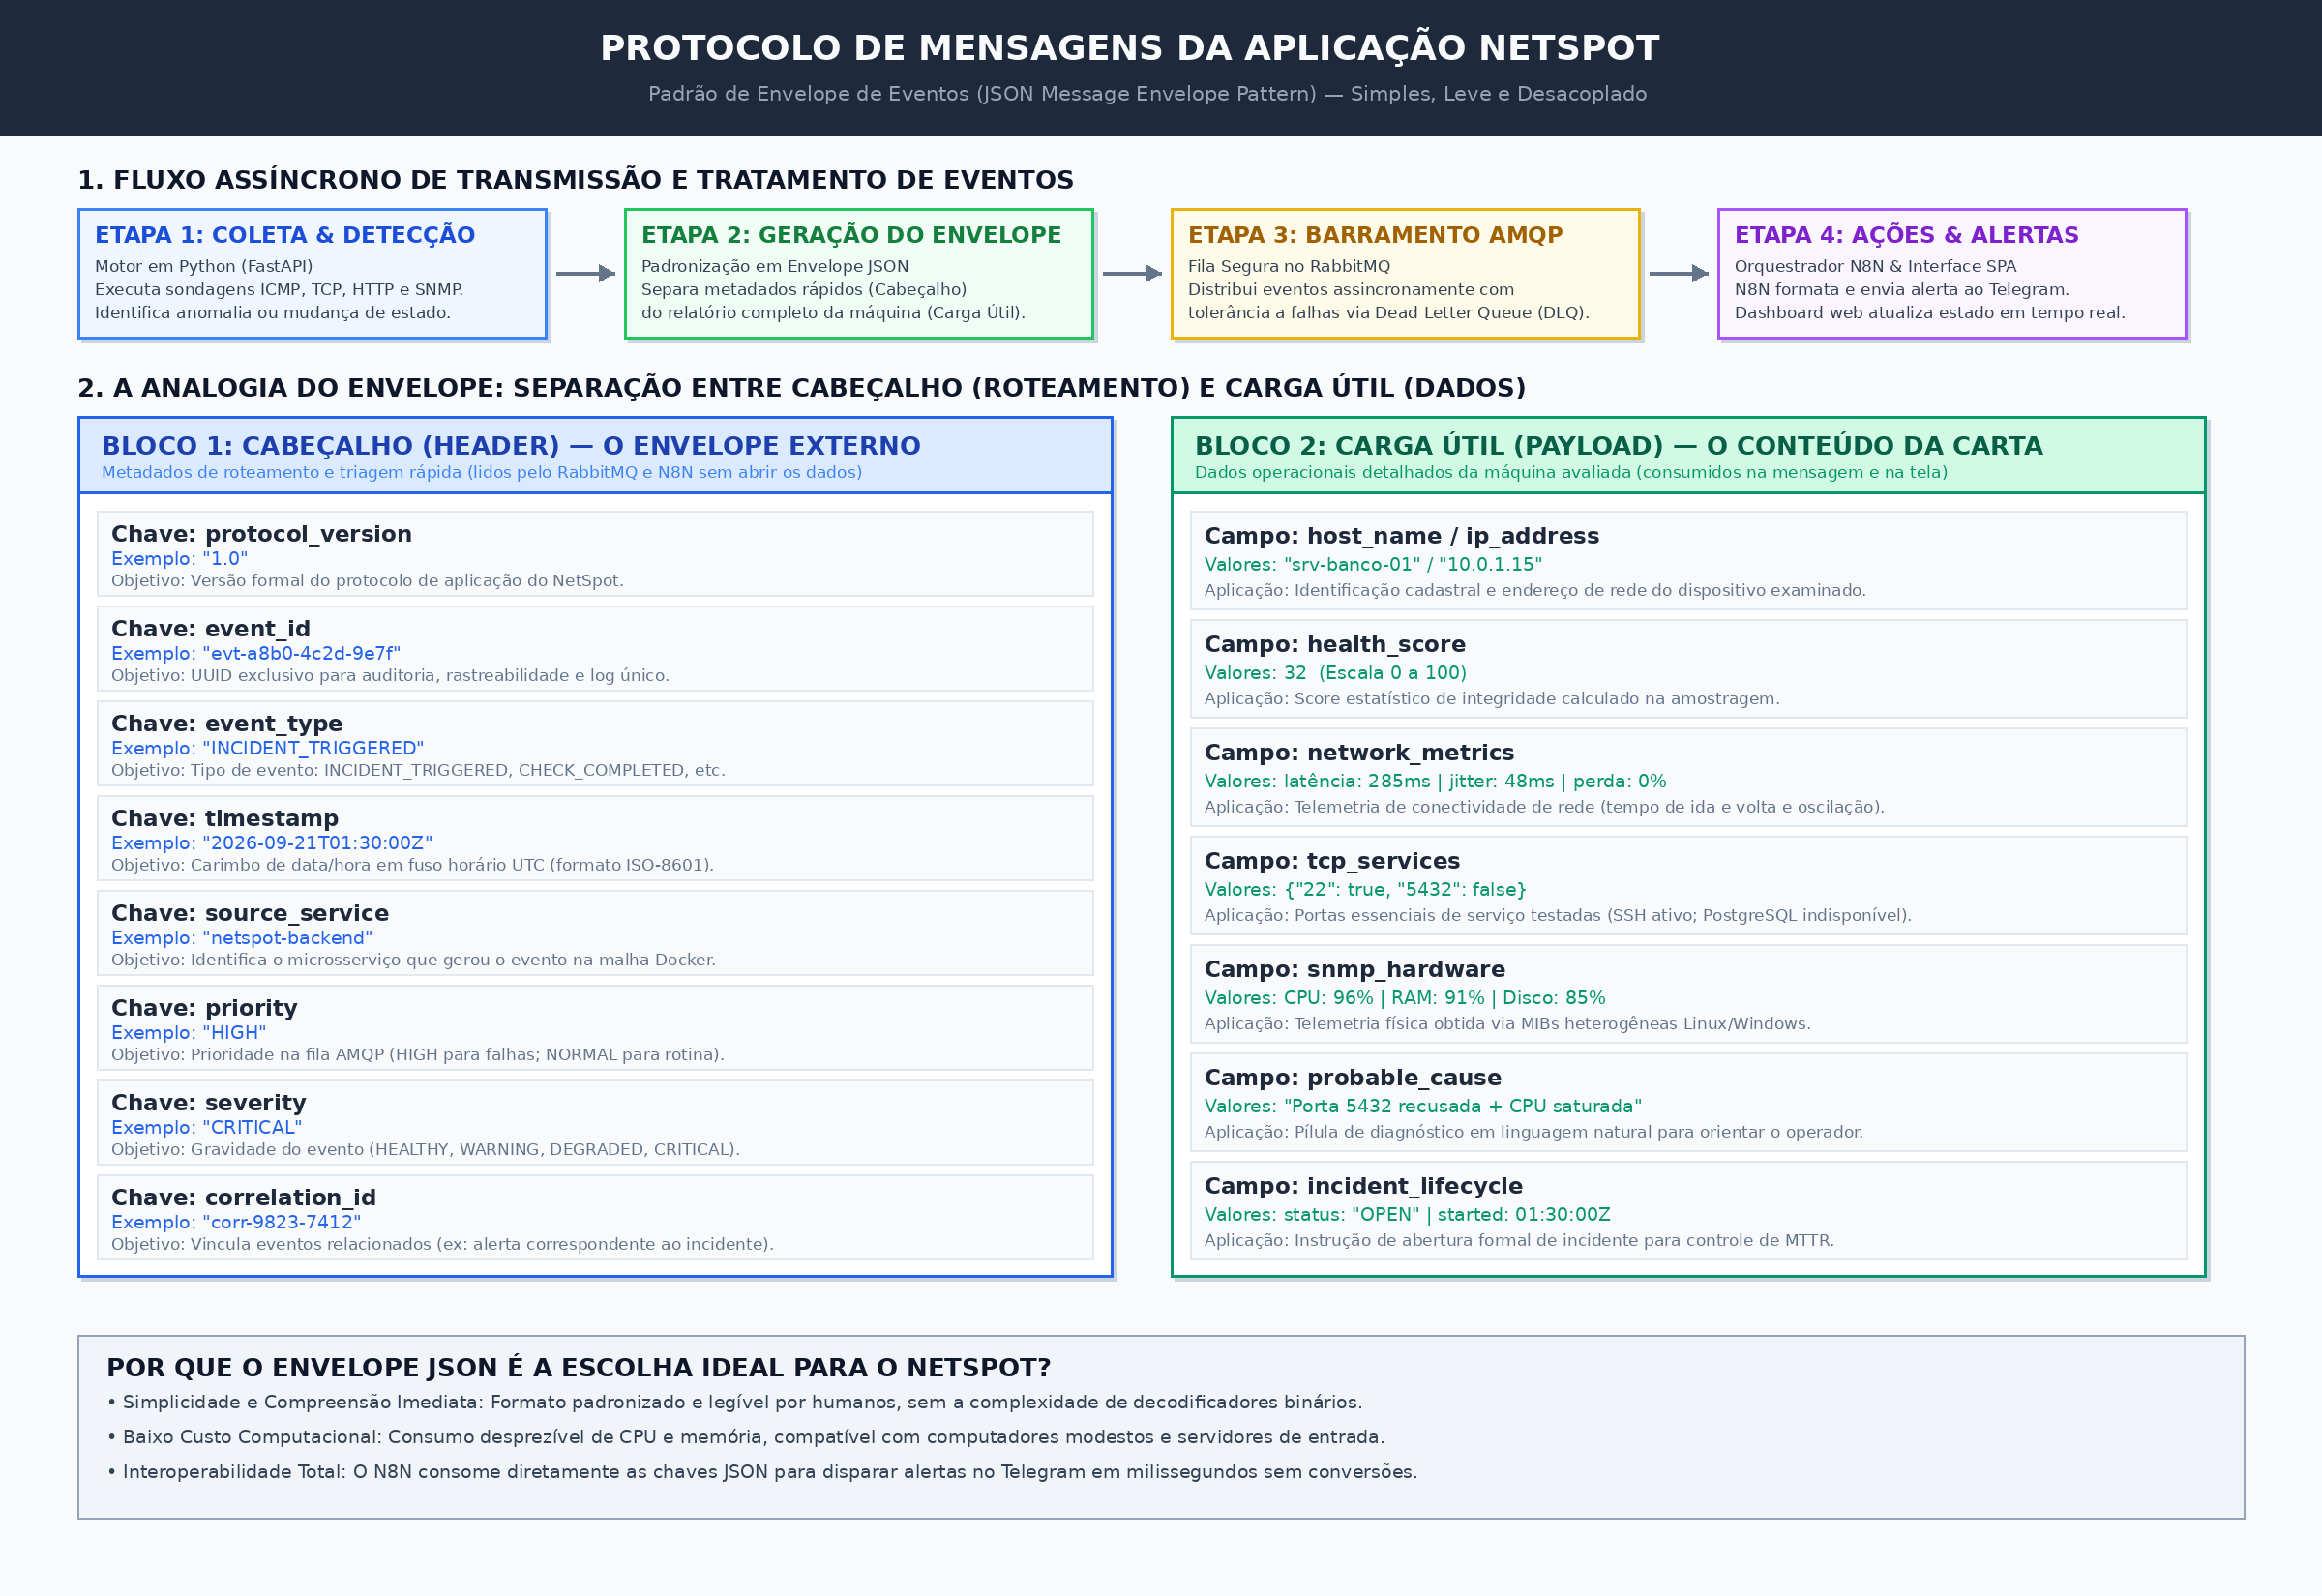
\includegraphics[width=0.98\textwidth]{protocolo_envelope_simplificado.png}
\fonte{Autoria própria (2026).}
\end{figure}

Para facilitar o entendimento conceitual, o protocolo pode ser compreendido através da \textbf{analogia com uma correspondência postal expressa}, dividida rigorosamente em duas partes complementares:

\begin{enumerate}[leftmargin=1.25cm]
\item \textbf{O Envelope Externo: Cabeçalho da Mensagem (\textit{Message Header})}: Assim como o envelope de uma carta física contém o remetente, o endereço do destinatário, o carimbo postal de data/hora e o selo de urgência, o cabeçalho do NetSpot reúne os metadados indispensáveis para roteamento e triagem rápida pelo RabbitMQ e N8N:
  \begin{itemize}
  \item \texttt{protocol\_version}: Versão formal da especificação de mensageria da aplicação (\texttt{1.0});
  \item \texttt{event\_id}: Identificador exclusivo universal (UUID) gerado na origem para rastreabilidade e auditoria em logs centralizados;
  \item \texttt{event\_type}: Natureza do evento emitido, permitindo a triagem imediata nas filas de mensageria (\texttt{INCIDENT\_TRIGGERED}, \texttt{CHECK\_COMPLETED}, \texttt{INCIDENT\_RESOLVED} ou \texttt{HEALTH\_DEGRADED});
  \item \texttt{timestamp}: Carimbo temporal exato da amostragem em fuso horário UTC (formato ISO-8601);
  \item \texttt{source\_service}: Nome do microsserviço que gerou o evento na malha containerizada (\texttt{netspot-backend});
  \item \texttt{priority}: Prioridade operacional no barramento AMQP (\texttt{HIGH} para abertura de incidentes e \texttt{NORMAL} para telemetria rotineira);
  \item \texttt{severity}: Classificação do grau de impacto no ativo (\texttt{HEALTHY}, \texttt{WARNING}, \texttt{DEGRADED} ou \texttt{CRITICAL});
  \item \texttt{correlation\_id}: Identificador para correlacionar eventos encadeados (ex.: associar o alarme de recuperação ao incidente original).
  \end{itemize}

\item \textbf{O Conteúdo da Carta: Carga Útil (\textit{Message Payload})}: Contém o relatório operacional completo e detalhado do dispositivo examinado, sendo aberto e processado apenas pelo consumidor final que precisa exibir ou notificar a ocorrência:
  \begin{itemize}
  \item \texttt{host\_name / ip\_address}: Identificação cadastral e endereço de rede do equipamento examinado;
  \item \texttt{health\_score}: Índice estatístico de integridade consolidado (0 a 100 pontos);
  \item \texttt{network\_metrics}: Indicadores de conectividade, incluindo tempo de resposta ICMP (\textit{latency\_ms}), oscilação de atraso (\textit{jitter\_ms}) e percentual de perda de pacotes;
  \item \texttt{tcp\_services}: Dicionário relacionando cada porta TCP monitorada com seu status booleano de resposta (ex.: SSH :22, PostgreSQL :5432);
  \item \texttt{snmp\_hardware}: Telemetria de hardware com os percentuais de uso de CPU, memória RAM, ocupação de disco e tráfego instantâneo em Bytes por segundo;
  \item \texttt{probable\_cause}: Diagnóstico em linguagem natural gerado pelo motor analítico (ex.: \textit{``Porta 5432 recusada + CPU saturada''}), orientando imediatamente a tomada de decisão da equipe técnica;
  \item \texttt{incident\_lifecycle}: Instruções de ciclo de vida do incidente (\texttt{OPEN} ou \texttt{CLOSED}) com duração acumulada da indisponibilidade.
  \end{itemize}
\end{enumerate}

Para ilustrar a simplicidade e a transparência operacional desse modelo, o trecho a seguir exemplifica uma mensagem real emitida durante a abertura de um incidente crítico:

\begin{verbatim}
{
  "header": {
    "protocol_version": "1.0",
    "event_id": "evt-a8b0-4c2d-9e7f",
    "event_type": "INCIDENT_TRIGGERED",
    "timestamp": "2026-09-21T01:30:00Z",
    "source_service": "netspot-backend",
    "priority": "HIGH",
    "severity": "CRITICAL",
    "correlation_id": "corr-9823-7412"
  },
  "payload": {
    "host_name": "srv-banco-01",
    "ip_address": "10.0.1.15",
    "health_score": 32,
    "network_metrics": {
      "ping_latency_ms": 285.4,
      "jitter_ms": 48.2,
      "packet_loss_pct": 0.0
    },
    "tcp_services": {
      "port_22": true,
      "port_5432": false
    },
    "snmp_hardware": {
      "cpu_pct": 96.5,
      "ram_pct": 91.2,
      "disk_pct": 85.0
    },
    "probable_cause": "Porta 5432 recusada + CPU saturada",
    "incident_action": "OPEN"
  }
}
\end{verbatim}

A Tabela \ref{tab:envelope_protocolo} sintetiza a estrutura do envelope de dados trafegado entre os microsserviços do NetSpot:

\begin{table}[H]
\centering
\caption{Estrutura simplificada do envelope de eventos do NetSpot}
\label{tab:envelope_protocolo}
\small
\begin{tabular}{@{}p{3.0cm}p{3.5cm}p{7.5cm}@{}}
\toprule
\textbf{Bloco Estrutural} & \textbf{Campo / Chave} & \textbf{Significado e Função Operacional} \\
\midrule
\textbf{Cabeçalho} & \texttt{protocol\_version} & Versão da especificação de mensageria da aplicação. \\
\textbf{(Header / Envelope)} & \texttt{event\_id} & Identificador UUID exclusivo para correlação de logs. \\
& \texttt{event\_type} & Tipo de evento (Incidente, Telemetria Periódica ou Alerta). \\
& \texttt{timestamp} & Horário exato da amostragem em fuso horário UTC. \\
& \texttt{priority} & Prioridade de despacho no barramento AMQP (\textit{High / Normal}). \\
& \texttt{severity} & Classificação de urgência (\textit{Critical}, \textit{Degraded} ou \textit{Healthy}). \\
\midrule
\textbf{Carga Útil} & \texttt{host\_name / ip} & Nome de cadastro e endereço IP do equipamento monitorado. \\
\textbf{(Payload / Carta)} & \texttt{health\_score} & Índice estatístico de saúde da máquina (0 a 100\%). \\
& \texttt{latency\_ms / jitter} & Tempo de resposta de ida e volta (RTT) e oscilação de atraso. \\
& \texttt{tcp\_ports} & Estado individual das portas de rede essenciais testadas. \\
& \texttt{snmp\_hardware} & Percentuais de consumo de CPU, memória RAM, disco e Bps. \\
& \texttt{probable\_cause} & Pílula diagnóstica que orienta a tomada de decisão da equipe. \\
\bottomrule
\end{tabular}
\fonte{Autoria própria (2026).}
\end{table}

A escolha do padrão de Envelope JSON em detrimento de protocolos binários de rede fundamenta-se em três vantagens técnicas decisivas para a proposta do NetSpot:
\begin{itemize}[leftmargin=1.25cm]
\item \textbf{Compreensão e Legibilidade Imediata}: O formato JSON é autoexplicativo e pode ser inspecionado diretamente na interface de gerenciamento do RabbitMQ sem a necessidade de analisadores de pacotes de baixo nível (como Wireshark ou tcpdump);
\item \textbf{Mínimo Custo Computacional}: As rotinas de serialização e parsing em Python e JavaScript operam com consumo imperceptível de CPU e memória RAM, preservando a capacidade de máquinas com recursos de hardware modestos;
\item \textbf{Interoperabilidade Direta com N8N e Telegram}: O orquestrador N8N absorve nativamente os campos do JSON, permitindo formatar e enviar notificações ricas para o Telegram em milissegundos, dispensando camadas intermediárias de conversão de dados.
\end{itemize}

\subsection{MECANISMOS DE AUTOCURA E RESILIÊNCIA (SELF-HEALING)}
Para assegurar operação contínua e tolerância a instabilidades em ambientes de produção, o NetSpot incorpora mecanismos avançados de autocura e engenharia de resiliência:

\subsubsection{Autocura do PostgreSQL}
O acesso ao banco de dados (\texttt{Backend/database.py}) é gerenciado por um pool auto-regenerativo no SQLAlchemy configurado com parâmetros de alta tolerância:
\begin{itemize}[leftmargin=1.25cm]
\item \texttt{pool\_pre\_ping=True}: Executa um teste de conectividade leve (\texttt{SELECT 1}) em cada conexão antes de liberá-la para execução de comandos SQL, descartando e reestabelecendo conexões mortas de forma transparente à aplicação;
\item \texttt{pool\_recycle=1800}: Descarta e renova conexões TCP ociosas a cada 30 minutos, impedindo encerramentos abruptos por firewalls intermediários;
\item \texttt{wait\_for\_database()}: Rotina de inicialização que executa até 15 tentativas de reconexão com \textit{backoff} exponencial caso o container do banco de dados ainda esteja inicializando durante a subida do Docker Compose.
\end{itemize}

\subsubsection{Autocura do Barramento RabbitMQ}
A comunicação com o broker AMQP (\texttt{Backend/mq\_manager.py}) utiliza o método \texttt{aio\_pika.connect\_robust()}. Uma tarefa em segundo plano (\texttt{\_monitor\_connection\_loop()}) avalia a cada 5 segundos a higidez da conexão. Em caso de interrupção na rede ou reinicialização do broker, o canal de comunicação é reconstruído automaticamente e todos os consumidores de filas são re-inscritos sem perda de contexto ou intervenção manual.

\subsubsection{As 6 Funcionalidades Avançadas de Engenharia de Resiliência}
O sistema consolida 6 padrões de engenharia de resiliência voltados à confiabilidade de missão crítica:

\begin{enumerate}[leftmargin=1.25cm]
\item \textbf{Diagnóstico de Saúde Nativo (\texttt{/healthz} + Docker Healthcheck)}: O endpoint \texttt{/healthz} afere a latência e o status do PostgreSQL e do RabbitMQ em tempo de execução. O Docker Compose associa a rota a uma verificação períodica (\texttt{CMD-SHELL}), reiniciando o container de forma autônoma caso ocorra travamento de processos.
\item \textbf{Pattern Circuit Breaker (Disjuntor de Polling)}: Implementado em \texttt{Backend/services/circuit\_breaker.py}. Ao detectar 5 falhas consecutivas em um host monitorado (\texttt{failure\_threshold = 5}), o disjuntor transita do estado \texttt{CLOSED} para \texttt{OPEN}. Durante a janela de 120 segundos, novos testes de ping, TCP e SNMP para este ativo são silenciados, prevenindo tempestades de pacotes, esgotamento de portas e bloqueio da tabela de conexões do sistema operacional. Decorrido o período, o estado muda para \texttt{HALF-OPEN}, permitindo um teste único de sondagem para restabelecer a operação normal caso o ativo tenha retornado.
\item \textbf{Dead Letter Queue (DLQ no RabbitMQ)}: Mensagens que encontram falhas sucessivas de processamento nos nós de notificação são encaminhadas para a troca de roteamento \texttt{netspot.dlx} e isoladas na fila segura \texttt{netspot.dlq}, garantindo taxa zero de perda de eventos (\textit{zero event loss}) durante falhas transitórias.
\item \textbf{Anti-Spam de Alertas e Supressão de Flapping Composta}: A função \texttt{is\_flapping\_suppressed()} (\texttt{Backend/notifications.py}) analisa as transições de estado em uma janela móvel de 5 minutos, particionando o controle por chave composta \texttt{host\_id:event\_type}. Essa abordagem garante que alertas de restabelecimento legítimos (\texttt{RECOVERY}) sejam entregues imediatamente ao Telegram sem atraso, enquanto notificações repetidas de oscilação transitória de queda (\texttt{DOWN}) são suprimidas após 4 ocorrências, eliminando a fadiga de alertas (\textit{Alert Fatigue}) na equipe do NOC.
\item \textbf{Graceful Shutdown (Desligamento Gracioso)}: O ciclo de vida da aplicação é orquestrado nativamente pelo servidor ASGI Uvicorn em conformidade com as boas práticas de microsserviços do \textit{12-Factor App}. Ao interceptar sinais POSIX de término (\texttt{SIGTERM} e \texttt{SIGINT}), o motor de execução suspende novos despachos no laço assíncrono, drena com segurança as mensagens em trânsito no barramento RabbitMQ (\texttt{aio\_pika}), aguarda a conclusão das checagens ativas e invoca o encerramento determinístico dos pools de conexões do PostgreSQL (\texttt{engine.dispose()}). Essa abordagem elimina interrupções forçadas por \textit{timeout} de container (\texttt{SIGKILL}), prevenindo corrupção de estado relacional e conexões zumbis no SGBD.
\item \textbf{Resiliência de Processos, Varredura SNMP e Otimização de Consultas}: Para evitar vazamento de descritores e saturação da tabela de processos do Linux (\textit{PID exhaustion}), a execução de comandos de rede assíncronos (como \texttt{ping}) é encapsulada em temporizadores rigorosos (\texttt{asyncio.wait\_for}) com término compulsório via sinal \texttt{SIGKILL} e coleta determinística com \texttt{proc.wait()}. No subsistema SNMP, o caminhamento de árvores MIB (\texttt{walk\_snmp}) implementa um teto de salvaguarda de 500 iterações para mitigar laços infinitos provocados por agentes anômalos. Adicionalmente, as APIs de telemetria histórica eliminam o padrão de gargalo $N+1$: a série temporal de disponibilidade dos últimos 60 minutos consolida os intervalos em uma única consulta SQL indexada com cômputo temporal em memória, reduzindo a latência de resposta do dashboard em mais de 90\%.
\end{enumerate}

\subsection{PROTOCOLOS E MOTOR SNMP MULTIPLATAFORMA}
O motor de coleta assíncrono do NetSpot executa verificações contínuas em múltiplos protocolos da pilha TCP/IP:
\begin{itemize}[leftmargin=1.25cm]
\item \textbf{ICMP Ping}: Medição precisa de latência de ida e volta (RTT em milissegundos) e diagnóstico de conectividade básica de camada de rede;
\item \textbf{TCP Check}: Teste de abertura de \textit{sockets} em portas arbitrárias (ex.: 22 para SSH, 80 para HTTP, 443 para HTTPS, 3306 para MySQL, 5432 para PostgreSQL), validando a disponibilidade do serviço de transporte;
\item \textbf{HTTP / HTTPS}: Envio de requisições GET/HEAD assíncronas com validação de código de status retornado (200 OK) e mensuração do tempo de resposta web;
\item \textbf{DNS}: Resolução de nomes de domínio com auditoria de registros tipo A e validação de consistência de TTL.
\end{itemize}

Para a coleta de telemetria profunda de hardware, o subsistema SNMP (\texttt{Backend/snmp/}) foi concebido sob uma arquitetura puramente assíncrona sobre a biblioteca PySNMP (arquitetura \textit{v3arch}), garantindo compatibilidade multiplataforma entre Linux e Windows sem bloqueio do \textit{event loop} do Python. O módulo opera através de três componentes especializados:

\begin{enumerate}[leftmargin=1.25cm]
\item \textbf{Cliente Assíncrono Puro (\texttt{snmp\_client.py})}: Encapsula as operações primitivas de consulta \texttt{get\_cmd} (SNMP GET) e \texttt{next\_cmd} (SNMP WALK) sobre transporte UDP assíncrono (\texttt{UdpTransportTarget}), configurado com tempo limite de 2 segundos (\texttt{timeout=2}) e até 2 retentativas (\texttt{retries=2}). Ao término de cada operação, o despachante de eventos é determinística e pontualmente finalizado (\texttt{snmp\_engine.close\_dispatcher()}), prevenindo vazamento de descritores de sockets no sistema operacional.
\item \textbf{Motor de Autodescoberta Heurística de OIDs (\texttt{snmp\_discovery.py})}: Quando um dispositivo cadastrado não responde aos OIDs padrão do catálogo, o NetSpot dispara um procedimento de descoberta profunda via caminhamento MIB (\texttt{walk\_snmp}):
  \begin{itemize}
  \item \textit{Descoberta de CPU}: Testa prioritariamente a MIB UCD-SNMP Idle (\texttt{1.3.6.1.4.1.2021.11.11.0}); em caso de ausência, varre a tabela Host-Resources Processor (\texttt{1.3.6.1.2.1.25.3.3.1.2}) e mapeia o primeiro núcleo ativo;
  \item \textit{Descoberta de Armazenamento e Partição Principal}: Varre a árvore de armazenamento (\texttt{1.3.6.1.2.1.25.2.3.1.3}), inspeciona as descrições textuais das unidades e extrai dinamicamente o índice correspondente à raiz (\texttt{/}) em sistemas Linux ou ao volume primário (\texttt{C:\textbackslash}) em estações Windows;
  \item \textit{Seleção da Melhor Interface de Rede}: Mapeia a tabela de interfaces de alta capacidade (\texttt{1.3.6.1.2.1.31.1.1.1.1}), descartando automaticamente pseudodispositivos de loopback (\texttt{lo}) e interfaces virtuais efêmeras de contêineres (\texttt{docker*}, \texttt{veth*}), priorizando dinamicamente interfaces físicas ethernet e sem fio (\texttt{eth*}, \texttt{enp*}, \texttt{ens*}, \texttt{wlan*}, \texttt{Ethernet}).
  \end{itemize}
\item \textbf{Resolução com Cache Local e Banco (\texttt{oid\_resolver.py} e \texttt{oid\_cache.py})}: Os OIDs mapeados para cada ativo são armazenados em um cache em memória de dois níveis com persistência relacional, evitando o custo computacional de re-escanear a árvore MIB a cada ciclo de amostragem.
\end{enumerate}

A Tabela \ref{tab:mapeamento_snmp} sintetiza o mapeamento comparativo de OIDs empregado pelo NetSpot para compatibilidade simultânea entre estações Linux e Windows:

\begin{table}[H]
\centering
\caption{Mapeamento comparativo de OIDs para Linux e Windows no NetSpot}
\label{tab:mapeamento_snmp}
\small
\begin{tabular}{@{}p{3.2cm}p{5.5cm}p{6.0cm}@{}}
\toprule
\textbf{Métrica de Hardware} & \textbf{Linux (UCD-SNMP-MIB / RFC 1213)} & \textbf{Windows (HOST-RESOURCES-MIB)} \\
\midrule
Uso de Processador (CPU) & \texttt{ssCpuIdle} (\texttt{.1.3.6.1.4.1.2021.11.11.0}) & \texttt{hrProcessorLoad} (\texttt{.1.3.6.1.2.1.25.3.3.1.2}) \\
Memória RAM & \texttt{memTotalReal} (\texttt{.4.5.0}) / \texttt{memAvailReal} (\texttt{.4.6.0}) & \texttt{hrStorageSize} / \texttt{hrStorageUsed} (\texttt{Memory}) \\
Armazenamento em Disco & \texttt{dskPercent} (\texttt{.1.3.6.1.4.1.2021.9.1.9.1}) & \texttt{hrStorageUsed} / \texttt{Size} (\texttt{C:\textbackslash}) \\
Tráfego de Rede (RX/TX) & \texttt{ifInOctets} / \texttt{ifOutOctets} (\texttt{.1.3.6.1.2.1.2.2.1}) & \texttt{ifInOctets} / \texttt{ifOutOctets} (\texttt{.1.3.6.1.2.1.2.2.1}) \\
\bottomrule
\end{tabular}
\fonte{Autoria própria (2026).}
\end{table}

A taxa instantânea de tráfego de rede em Bits por segundo (bps) é derivada pela Equação \ref{eq:vazao_bps}, computada pela multiplicação da variação de octetos por 8 (conversão de bytes para bits) e dividida pelo intervalo decorrido ($\Delta t = t_2 - t_1$):
\begin{equation}
\label{eq:vazao_bps}
\text{Vazão (bps)} = (\Delta\text{Octetos} * 8) / \Delta t
\end{equation}

Para prevenir distorções na telemetria decorrentes do estouro de contadores acumulativos de rede (\textit{counter rollover/overflow}) — comum em contadores de 32 bits (\texttt{Counter32}), que atingem seu valor máximo de 4.294.967.295 octetos em poucas horas em links de alta velocidade —, o algoritmo implementado em \texttt{Backend/snmp\_engine.py} calcula a variação conforme a Equação \ref{eq:delta_octets}:
\begin{equation}
\label{eq:delta_octets}
\Delta\text{Octetos} = \text{Octetos}_{\text{atual}} - \text{Octetos}_{\text{anterior}}
\end{equation}
Caso ocorra o estouro do contador de 32 bits ($\text{Octetos}_{\text{atual}} < \text{Octetos}_{\text{anterior}}$), o valor da variação é corrigido somando-se a capacidade total do contador ($4.294.967.296$):
\begin{equation*}
\Delta\text{Octetos} = (4294967296 - \text{Octetos}_{\text{anterior}}) + \text{Octetos}_{\text{atual}}
\end{equation*}

Adicionalmente, para preservar a estabilidade operacional contra hosts que desabilitaram o serviço SNMP ou que apresentem instabilidade intermitente de credenciais, o motor incorpora um algoritmo de \textit{Backoff Exponencial} (\texttt{register\_snmp\_failure()}): ao atingir 3 falhas consecutivas de consulta, o ativo entra em pausa temporária de checagem SNMP de 300 segundos ($5$ minutos), dobrando progressivamente a cada novo ciclo de insucesso até o teto máximo de 3.600 segundos ($1$ hora), poupando tráfego de rede e consumo de CPU no servidor de monitoramento.

\subsection{MODELAGEM MATEMÁTICA E MÉTRICAS NOC}
A análise de telemetria do NetSpot apoia-se em formulações aritméticas simples implementadas no módulo \texttt{Backend/metrics.py} e correlacionadas em \texttt{Backend/routes/hosts.py}:

\subsubsection{Algoritmo do Health Score (Score de Saúde)}
O \textit{Health Score} reflete o índice consolidado de integridade operacional do ativo, computado dinamicamente em uma escala de 0 a 100 pontos pela razão entre a pontuação obtida e a pontuação máxima possível, conforme a Equação \ref{eq:health_score_calc}:
\begin{equation}
\label{eq:health_score_calc}
\text{Health Score} = (\text{Pontos Obtidos} / \text{Pontos Máximos}) * 100
\end{equation}
onde a pontuação obtida corresponde à soma das pontuações dos protocolos monitorados:
\begin{equation*}
\text{Pontos Obtidos} = \text{Pontos}_{\text{ICMP}} + \text{Pontos}_{\text{TCP}} + \text{Pontos}_{\text{HTTP}}
\end{equation*}

A pontuação compõe-se das seguintes regras operacionais implementadas no backend:
\begin{itemize}[leftmargin=1.25cm]
\item \textbf{Conectividade ICMP ($P_{\text{ICMP}}$)}: Concede 30 pontos básicos em caso de sucesso no ping. Adiciona bônus integral de 15 pontos se a latência for inferior a 100 ms (incluindo o tratamento exato de containers locais e enlaces de rede de altíssima velocidade com RTT medido de 0.0 ms, garantindo pontuação máxima sem distorções numéricas), ou bônus de 8 pontos se a latência situar-se entre 100 e 300 ms.
\item \textbf{Tratamento Compensatório de Firewall ICMP}: Em redes corporativas e acadêmicas, é frequente que roteadores de borda ou firewalls com inspeção de estado (\textit{Stateful Inspection}) descartem intencionalmente pacotes ICMP \textit{Echo Request} (Tipo 8) para ocultar o host contra varreduras de perímetro, mantendo todavia portas L4 (TCP) ou L7 (HTTP) totalmente acessíveis. Para evitar o fenômeno deletério de falso-positivo de host inativo, o algoritmo detecta essa contingência conforme a Equação \ref{eq:icmp_firewall_comp}:
\begin{equation}
\label{eq:icmp_firewall_comp}
\text{ICMP Bloqueado} = (1 - \text{Sucesso}_{\text{Ping}}) * (\text{Sucesso}_{\text{TCP}} + \text{Sucesso}_{\text{HTTP}})
\end{equation}
onde cada indicador assume valor 1 para sucesso e 0 para falha. Caso o resultado seja maior que zero (indicando falha de ping simultânea ao êxito em portas TCP ou HTTP), o sistema não penaliza a saúde do equipamento, concedendo o sucesso efetivo da conectividade com latência neutra compensatória de 80 ms.
\item \textbf{Serviços TCP ($P_{\text{TCP}}$)}: Concede 30 pontos caso as portas de transporte configuradas respondam com sucesso no \textit{handshake}.
\item \textbf{Serviços Web HTTP ($P_{\text{HTTP}}$)}: Concede 25 pontos em caso de resposta 200 OK, com acréscimo de 10 pontos de bônus caso o tempo de resposta seja inferior a 500 ms. Aplica penalidade de $-20$ pontos para respostas da família 5xx (erros internos de servidor) e penalidade de $-10$ pontos para a família 4xx (erros de cliente ou recursos inexistentes).
\end{itemize}

O score resultante determina a classificação de severidade operacional do ativo:
\begin{itemize}[leftmargin=1.25cm]
\item \textbf{Saudável (\texttt{HEALTHY})}: $\text{HS} \ge 85$;
\item \textbf{Atenção (\texttt{WARNING})}: $65 \le \text{HS} < 85$;
\item \textbf{Degradado (\texttt{DEGRADED})}: $40 \le \text{HS} < 65$;
\item \textbf{Crítico (\texttt{CRITICAL})}: $\text{HS} < 40$.
\end{itemize}

\subsubsection{Cálculo de Disponibilidade e SLA Móvel (Rolling SLA)}
O NetSpot calcula o índice percentual de conformidade de SLA (\textit{Service Level Agreement}) através da Equação \ref{eq:sla_rolling}, que formaliza janelas móveis deslizantes (\textit{rolling window}) compostas pelas últimas $K = 50$ checagens registradas no banco de dados para cada protocolo individualmente (Ping, TCP e HTTP):
\begin{equation}
\label{eq:sla_rolling}
\text{SLA Móvel} = (\text{Checagens com Sucesso} / \text{Total de Checagens}) * 100
\end{equation}
A preservação de janelas móveis no nível de aplicação permite absorver intermitências transitórias sem descaracterizar a confiabilidade estatística de longo prazo do equipamento.

\subsubsection{Algoritmo de SLA por União de Intervalos Temporais (Interval Merging)}
Para além das janelas pontuais de amostras, o cálculo do SLA histórico consolidado da infraestrutura implementa o \textbf{Algoritmo de União de Intervalos de Tempo (\textit{Interval Merging})} (\texttt{Backend/metrics.py}). Ferramentas simplistas costumam somar isoladamente a duração de cada incidente ocorrido em uma janela temporal; todavia, quando falhas afetam múltiplos serviços simultaneamente no mesmo host (ex.: queda simultânea de portas TCP e HTTP), a simples soma aritmética duplica o tempo computado, gerando distorções no cálculo.

Para solucionar essa incompatibilidade, o NetSpot formaliza o cálculo ordenando os intervalos temporais de incidentes $[\text{Início}, \text{Fim}]$ e fundindo os segmentos contíguos ou sobrepostos para calcular a duração real de indisponibilidade conforme a Equação \ref{eq:interval_merging}:
\begin{equation}
\label{eq:interval_merging}
\text{Downtime Total} = (\text{Fim}_1 - \text{Início}_1) + (\text{Fim}_2 - \text{Início}_2) + \dots + (\text{Fim}_k - \text{Início}_k)
\end{equation}
onde cada par $(\text{Fim}_i - \text{Início}_i)$ representa a duração de cada intervalo de indisponibilidade após a união dos segmentos sobrepostos. A disponibilidade real do ativo em uma janela de observação de tempo total $T$ é expressa pela Equação \ref{eq:sla_consolidado}:
\begin{equation}
\label{eq:sla_consolidado}
\text{SLA Consolidado} = ((\text{Tempo Total} - \text{Downtime Total}) / \text{Tempo Total}) * 100
\end{equation}
assegurando precisão métrica auditável e em estrita consonância com os contratos formais de nível de serviço exigidos em ambientes corporativos.

\subsubsection{Mensuração Formal de Jitter (Variação Estatística de Latência)}
O \textit{Jitter} de rede é medido através da Equação \ref{eq:jitter_calc}, que obtém a média aritmética das variações absolutas de latência entre pares sucessivos de amostras em uma janela de $M = 10$ medições válidas de RTT, em consonância com os preceitos da RFC 3550 \cite{schulzrinne2003rfc3550}:
\begin{equation}
\label{eq:jitter_calc}
\text{Jitter} = (\text{Diferença}_1 + \text{Diferença}_2 + \dots + \text{Diferença}_k) / \text{Total de Pares}
\end{equation}
onde cada diferença é calculada pela variação absoluta entre amostras consecutivas:
\begin{equation*}
\text{Diferença}_i = |\text{Latência}_{i+1} - \text{Latência}_i|
\end{equation*}
Essa formulação permite capturar variações anômalas no enfileiramento de pacotes nos roteadores intermediários antes mesmo que ocorra descarte efetivo por estouro de buffer (\textit{bufferbloat}).

\subsubsection{Análise de Tendência por Regressão Linear (OLS) e Causa Provável}
Para antecipar degradações severas antes da interrupção completa do serviço, o módulo \texttt{Backend/metrics.py} aplica o método dos Mínimos Quadrados Ordinários (\textit{Ordinary Least Squares} -- OLS) sobre a série temporal das últimas $N$ latências válidas ($N \ge 5$, janela padrão $N = 10$). A inclinação da reta de ajuste linear (\textit{slope}) é expressa de forma simplificada pela Equação \ref{eq:ols_slope}:
\begin{equation}
\label{eq:ols_slope}
\text{Slope} = \text{Numerador} / \text{Denominador}
\end{equation}
onde o numerador e o denominador são computados pelas variações em relação às médias aritméticas ($\bar{x}$ para o tempo e $\bar{L}$ para a latência):
\begin{equation*}
\text{Numerador} = ((x_1 - \bar{x}) * (L_1 - \bar{L})) + \dots + ((x_N - \bar{x}) * (L_N - \bar{L}))
\end{equation*}
\begin{equation*}
\text{Denominador} = ((x_1 - \bar{x}) * (x_1 - \bar{x})) + \dots + ((x_N - \bar{x}) * (x_N - \bar{x}))
\end{equation*}
onde $x_i = i$ representa o índice ordinal discreto da amostra temporal, $L_i$ a latência observada, e $\bar{x}$, $\bar{L}$ denotam as respectivas médias aritméticas. A interpretação operacional do coeficiente angular obtido orienta a classificação preventiva:

\begin{itemize}[leftmargin=1.25cm]
\item \textbf{Tendência de Latência de Rede (ICMP e TCP)}:
  \begin{itemize}
  \item $\text{slope} > 40$: Degradação Rápida (\texttt{FAST\_DEGRADING}) -- crescimento abrupto de latência por saturação de enlace;
  \item $15 < \text{slope} \le 40$: Degradação (\texttt{DEGRADING}) -- tendência sustentada de enfileiramento;
  \item $\text{slope} < -15$: Recuperação (\texttt{IMPROVING}) -- esvaziamento de filas e restabelecimento da vazão;
  \item Demais casos: Estável (\texttt{STABLE}).
  \end{itemize}
\item \textbf{Tendência de Latência Web HTTP}:
  \begin{itemize}
  \item $\text{slope} < 10$: Estável (\texttt{STABLE});
  \item $10 \le \text{slope} < 40$: Ascendente (\texttt{RISING});
  \item $40 \le \text{slope} < 80$: Degradando (\texttt{DEGRADING});
  \item $\text{slope} \ge 80$: Crítico (\texttt{CRITICAL}).
  \end{itemize}
\end{itemize}

Complementarmente, a função \texttt{infer\_probable\_cause()} (\texttt{Backend/routes/hosts.py}) correlaciona esses vetores analíticos em uma árvore de decisão determinística de alta performance:
\begin{enumerate}[leftmargin=1.25cm]
\item \textbf{Atalho de Alto Desempenho (\textit{Fast-Path})}: Hosts saudáveis em estado \texttt{UP}, com ping responsivo, sem incidentes e com recursos locais abaixo de 90\% são rotulados instantaneamente como ``Operação normal'', sem onerar o banco de dados com varreduras recursivas;
\item \textbf{Diagnóstico de Firewall}: Se a Equação \ref{eq:icmp_firewall_comp} for satisfeita, emite o diagnóstico transparente ``ICMP bloqueado por firewall / Serviço operando normalmente'';
\item \textbf{Isolamento de Indisponibilidade (\texttt{DOWN})}: Segrega a falha em categorias precisas: ``Falha na resolução DNS'', ``Serviço HTTP instável (HTTP 5xx)'', ``Porta TCP indisponível'' ou ``Host sem resposta ICMP'';
\item \textbf{Diagnóstico de Sobrecarga e Instabilidade}: Identifica esgotamento de hardware por SNMP (CPU $\ge 95\%$, RAM $\ge 92\%$ ou Disco $\ge 95\%$) gerando ``Sobrecarga de recursos locais (CPU/RAM/Disco)'', ou variações anômalas de rede ($\text{Jitter} \ge 120$ ms ou $\text{SLA} < 95\%$) gerando ``Instabilidade de rede (jitter/perda)''.
\end{enumerate}

\subsection{FLUXOGRAMA DE DECISÕES E ORQUESTRAÇÃO DE EVENTOS AMQP}
O ciclo de vida operacional do NetSpot fundamenta-se nos preceitos de Arquitetura Orientada a Eventos e Padrões de Integração Corporativa \cite{hohpe2004enterprise}, estruturado de forma desacoplada através do barramento de mensageria assíncrona RabbitMQ, orquestrado pela classe \texttt{QueueManager} (\texttt{Backend/mq\_manager.py}), conforme ilustrado no fluxograma da Figura \ref{fig:fluxograma_decisoes}.

\begin{figure}[H]
\centering
\caption{Fluxograma das decisões e orquestração de eventos}
\label{fig:fluxograma_decisoes}
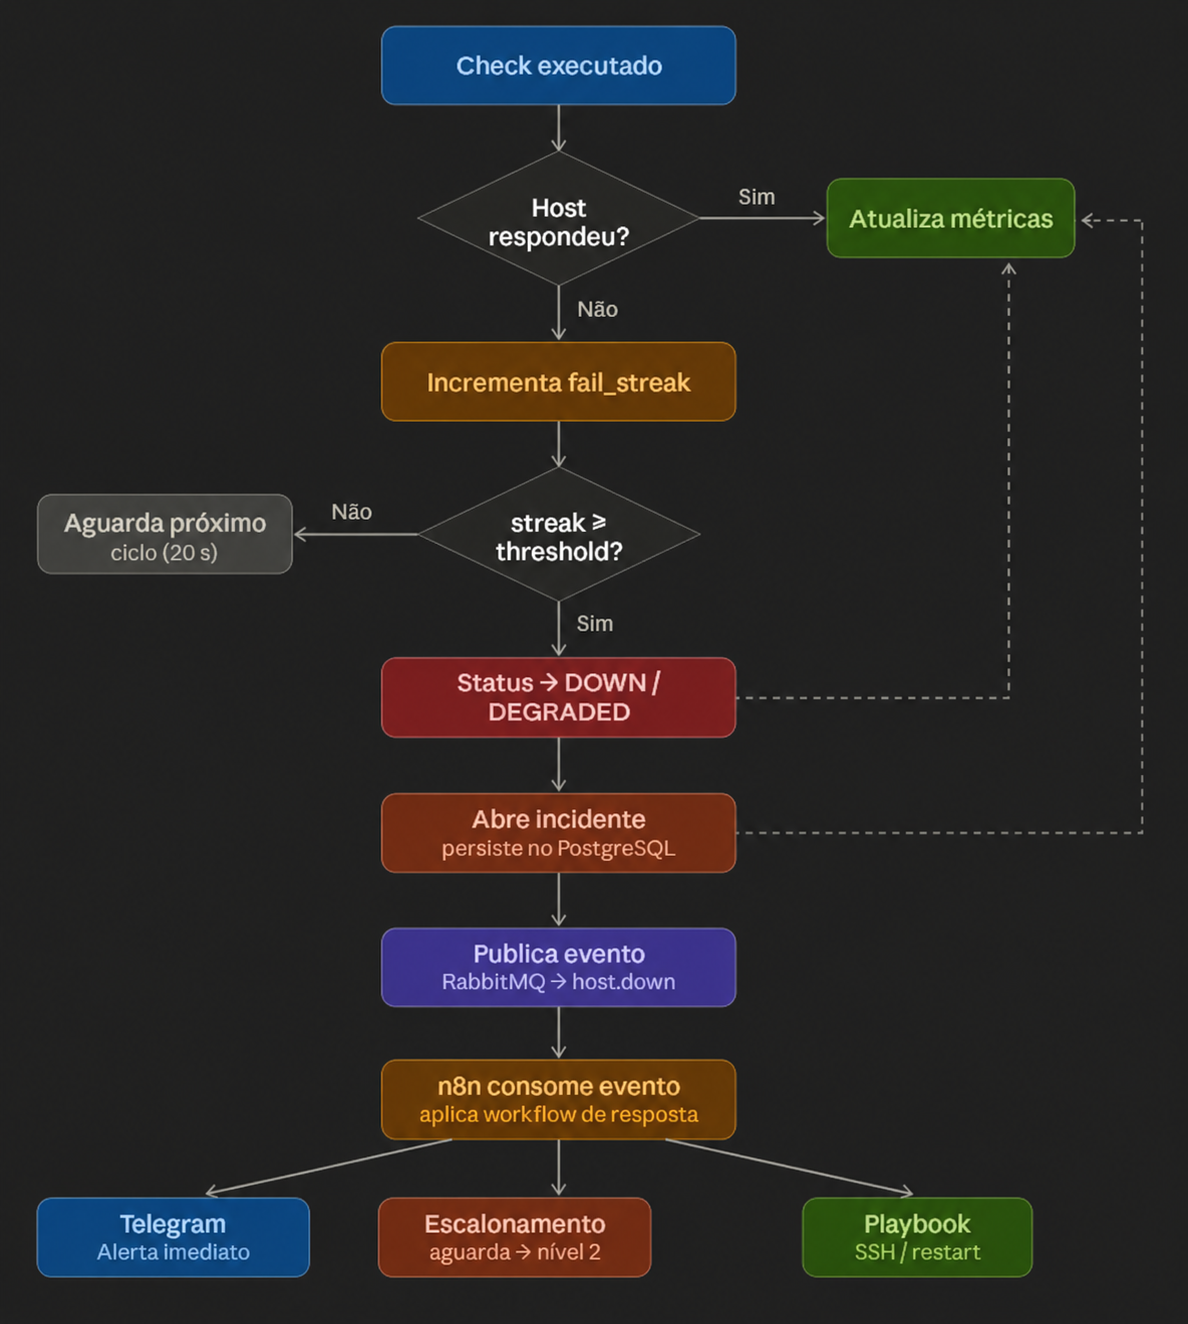
\includegraphics[height=0.68\textheight,width=0.88\textwidth,keepaspectratio]{image6.png}
\fonte{Autoria própria (2026).}
\end{figure}

A arquitetura de mensageria assenta-se em três pilares fundamentais de confiabilidade:
\begin{itemize}[leftmargin=1.25cm]
\item \textbf{Filas Duráveis e Mensagens Persistentes}: O agendador enfileira tarefas de sondagem na fila durável \texttt{netspot.host\_checks}, enquanto as transições de estado e alarmes são publicados na fila \texttt{netspot.notifications}. Todas as mensagens utilizam modo de entrega persistente (\texttt{DeliveryMode.PERSISTENT}), assegurando que nenhuma notificação seja perdida mesmo em caso de reinício intempestivo do broker;
\item \textbf{Controle de Fluxo e Dead Letter Queue (DLQ)}: O canal AMQP configura limite de pré-busca (\texttt{prefetch\_count=10}), impedindo o congestionamento de memória no consumidor assíncrono. Em caso de falhas irrecuperáveis no processamento de mensagens, os eventos são automaticamente roteados via \textit{Dead Letter Exchange} (\texttt{netspot.dlx}) para a fila de isolamento \texttt{netspot.dlq}, permitindo auditoria forense sem interromper o fluxo operacional contínuo;
\item \textbf{Monitor de Autocura de Conexão (\textit{Self-Healing Connection})}: O método \texttt{\_monitor\_connection\_loop()} executa um laço concorrente contínuo a cada 5 segundos. Caso identifique o fechamento acidental da conexão TCP ou do canal com o broker, o sistema aciona rotinas de reconexão automática exponencial e reinscreve transparentemente todos os consumidores de tarefas.
\end{itemize}

A gestão de alertas incorpora um algoritmo nativo de \textit{Anti-Flapping} com janela de amortecimento (\textit{cooldown}) parametrizável: quando um nó sofre instabilidades físicas repetidas (transitando ciclicamente entre \texttt{UP} e \texttt{DOWN}), o sistema abre o incidente formal no banco de dados e notifica o primeiro evento, suprimindo mensagens redundantes sucessivas dentro do período de histerese para proteger os operadores contra fadiga de alertas (\textit{alert fatigue}). As mensagens estruturadas são consumidas pelo N8N através de webhooks autenticados, formatadas em Markdown com ícones contextuais de severidade (Crítico/DOWN, Atenção/DEGRADED, Restabelecido/UP) e despachadas para canais do Telegram.

A gestão do ciclo de vida dos dados históricos no PostgreSQL é governada pelo módulo de retenção parametrizável (\texttt{NETSPOT\_RETENTION\_DAYS}), operando como um requisito não-funcional de sustentabilidade e desempenho contínuo do banco relacional. Um \textit{worker} assíncrono executa limpezas periódicas através de comandos SQL \texttt{DELETE} atômicos orientados por uma data de corte (\textit{cutoff}): expurgam-se registros de checagens pontuais (\texttt{checks}), métricas de telemetria SNMP (\texttt{snmp\_metrics}) e alertas resolvidos anteriores ao limite temporal definido, além de expurgar incidentes já concluídos (\texttt{incidents}). O dimensionamento padrão de 30 dias assegura um histórico operacional suficiente para análises estatísticas de disponibilidade sem comprometer a volumetria de disco, ao passo que a atribuição do valor \texttt{0} desativa a purga para cenários que exijam arquivamento perene.

\subsection{INTERFACE DO USUÁRIO (FRONTEND SPA) E EXPERIÊNCIA DO USUÁRIO (UX/UI)}
A interface de visualização do NetSpot foi inteiramente desenvolvida sob a filosofia de \textit{Single Page Application} (SPA), utilizando HTML5 semântico, CSS Vanilla com propriedades customizadas (\textit{CSS Variables}) e JavaScript moderno (ES6+ assíncrono). A arquitetura visual prioriza a clareza de dados em operações críticas de NOC, oferecendo alta densidade de informação sem sobrecarregar cognitivamente o operador.

\subsubsection{Design System Dual (Dark and White Theme) e Ergonomia Visual}
A estética do sistema apoia-se em um \textit{Design System} responsivo com suporte nativo a dois temas cromáticos (\textit{Dark and White Theme}), inspirado nas diretrizes visuais dos produtos de infraestrutura do Google:
\begin{itemize}[leftmargin=1.25cm]
\item \textbf{Tema Escuro (Dark Glassmorphism)}: Emprega superfícies em tons de cinza profundo (\texttt{\#121824} e \texttt{\#1a2332}), fundos translúcidos com efeito de desfoque (\textit{backdrop-filter: blur(12px)}), bordas sutis de 1 pixel e elementos em contraste balanceado para mitigar a fadiga ocular em salas de monitoramento contínuo;
\item \textbf{Tema Claro (Clean White)}: Apresenta superfícies brancas com contrastes neutros suaves, garantindo legibilidade em ambientes de alta luminosidade natural;
\item \textbf{Alternância Dinâmica e Persistência}: O cabeçalho abriga um botão em formato de pílula animada com ícones dinâmicos de sol e lua. A preferência do operador é persistida no \texttt{localStorage}, sendo aplicada instantaneamente no carregamento da página através de um script síncrono no \texttt{<head>}, impedindo oscilações de brilho (\textit{flash of unstyled theme}).
\end{itemize}

A tipografia utiliza as famílias \textit{Roboto} e \textit{Open Sans} via Google Fonts, provendo hierarquia clara entre títulos, métricas numéricas em negrito e rótulos secundários.

\subsubsection{Painel de Resumo Geral (Overview KPI Grid)}
No topo do painel principal, localiza-se o componente de resumo executivo da rede (\texttt{dashboardSummary}), que calcula e exibe em tempo real:
\begin{enumerate}[leftmargin=1.25cm]
\item \textbf{Hosts Cadastrados}: Volume total de ativos gerenciados na infraestrutura;
\item \textbf{Hosts Online}: Total de equipamentos em estado \texttt{UP} com taxa de disponibilidade plena;
\item \textbf{Hosts Offline}: Contagem de ativos indisponíveis (\texttt{DOWN});
\item \textbf{Hosts Degradados}: Dispositivos operando sob instabilidade (\texttt{DEGRADED});
\item \textbf{Taxa Média de Disponibilidade}: Índice percentual consolidado da infraestrutura;
\item \textbf{Incidentes Abertos}: Alerta visual imediato quando há falhas ativas na rede.
\end{enumerate}

\subsubsection{Cadastro e Edição Flexível de Ativos}
O formulário de cadastro permite ao operador parametrizar de forma granular o perfil de monitoramento de cada host:
\begin{itemize}[leftmargin=1.25cm]
\item Identificação por Nome e Endereço IP / FQDN;
\item Campo para URL HTTP/HTTPS com \textit{switch} de ativação de checagem web;
\item Mapeamento dinâmico de portas TCP: através de uma interface interativa com botão de adição rápida (\texttt{+}), o operador pode cadastrar uma lista arbitrária de portas de transporte (ex.: 80, 443, 22, 5432) a serem testadas individualmente por socket;
\item Parametrização SNMP: chave de habilitação e definição da comunidade de leitura (\textit{community string}, padrão \texttt{netspot}).
\end{itemize}
Um modal de edição correspondente (\texttt{editModal}) possibilita a reconfiguração em tempo de execução dos parâmetros operacionais sem necessidade de recriação do ativo.

\subsubsection{Módulo de Descoberta Automática de Rede (LAN Discovery)}
O sistema incorpora um motor nativo de varredura assíncrona de sub-redes locais via endpoint \texttt{/network/discover}:
\begin{itemize}[leftmargin=1.25cm]
\item \textbf{Varredura CIDR}: O operador informa uma faixa de endereçamento (ex.: \texttt{192.168.1.0/24}). O backend valida a segurança da requisição, aceitando máscaras de até \texttt{/20} (limite máximo de 4.096 endereços simultâneos para evitar sobrecarga de hardware);
\item \textbf{Descoberta e Seleção}: Uma requisição de sondagem varre os endereços ativos. Os nós responsivos são exibidos em uma lista com caixas de seleção (\textit{checkboxes});
\item \textbf{Importação em Lote Inteligente}: O acionamento do botão \textit{Adicionar selecionados} dispara o endpoint \texttt{/network/import}, que cadastra os equipamentos no banco de dados habilitando automaticamente o monitoramento SNMP e ICMP. Caso o dispositivo já tenha constado anteriormente no sistema em estado inativo, o motor reativa o ativo preservando a integridade histórica.
\end{itemize}

\subsubsection{Barra de Filtragem e Busca Instantânea}
Para permitir localização imediata de ativos em redes com dezenas de nós, o painel dispõe de:
\begin{itemize}[leftmargin=1.25cm]
\item \textbf{Busca Textual}: Campo reativo que filtra os cartões de host em tempo real conforme a digitação do operador, aceitando correspondências parciais por nome do equipamento ou endereço IP;
\item \textbf{Filtro por Estado Operacional}: Seletor \textit{dropdown} que segrega os ativos nas categorias \textit{Todos os Status}, \textit{Online} (verde), \textit{Offline} (vermelho) e \textit{Degradado} (amarelo).
\end{itemize}

\subsubsection{Arquitetura de Flip Cards 3D (3 Faces por Card de Host)}
A visualização principal dos dispositivos organiza-se em um \textit{grid} responsivo fixado em 3 colunas no Desktop (adaptando-se para 2 colunas em tablets e 1 em smartphones). Cada ativo é renderizado como um cartão multifuncional interativo de 3 faces com alternância suave:

\begin{enumerate}[leftmargin=1.25cm]
\item \textbf{Face 1 (Resumo Operacional)}: Exibe o cabeçalho com indicador luminoso pulsante do status atual (\texttt{UP}, \texttt{DOWN} ou \texttt{DEGRADED}), badge de severidade com símbolo de saúde, identificação de incidente aberto, disponibilidade calculada nos últimos 10 minutos, carimbo temporal do último teste, resumo das portas TCP sob monitoramento, status do probe web com código de retorno, tendência HTTP com setas visuais direcionais e a pílula diagnóstica de \textit{Causa Provável} (\textit{Probable Cause});
\item \textbf{Face 2 (Telemetria de Rede e SLA)}: Apresenta o detalhamento analítico de conectividade, dividindo a taxa de sucesso (SLA móvel de 50 amostras) individualmente para Ping, TCP e HTTP, a oscilação de latência (Jitter em milissegundos) para cada protocolo e a relação em tempo real de cada porta TCP aberta com respectivo RTT e rótulo de erro em caso de falha;
\item \textbf{Face 3 (Telemetria de Hardware SNMP)}: Reúne medidores KPI para carga de processamento de CPU (\%), ocupação de memória RAM (\%) e uso de partição de disco (\%) com barras dinâmicas com código de cores (verde $<60\%$, amarelo $60\text{--}80\%$, vermelho $>80\%$). Inclui o painel de tráfego de interface em Bytes por segundo (Bps) com barras proporcionais de Download (RX) e Upload (TX), além de renderizar gráficos temporais interativos alimentados pela biblioteca \textbf{Chart.js}.
\end{enumerate}

O topo de cada cartão disponibiliza uma barra de ações rápidas com ícones SVG vetoriais para visualização do histórico de checagens, abertura de gráficos de latência, abertura de gráficos SNMP, gráficos de disponibilidade por tipo, edição cadastral e exclusão.

A Figura~\ref{fig:painel_dashboard} apresenta a interface operacional do NetSpot em modo escuro (\textit{Dark Theme}), evidenciando a barra superior com os indicadores executivos de saúde da rede e a disposição dos cartões multifuncionais nas suas respectivas faces de telemetria.

\begin{figure}[H]
\centering
\caption{Painel de monitoramento do NetSpot em modo escuro com indicadores de desempenho e cartões multifuncionais}
\label{fig:painel_dashboard}
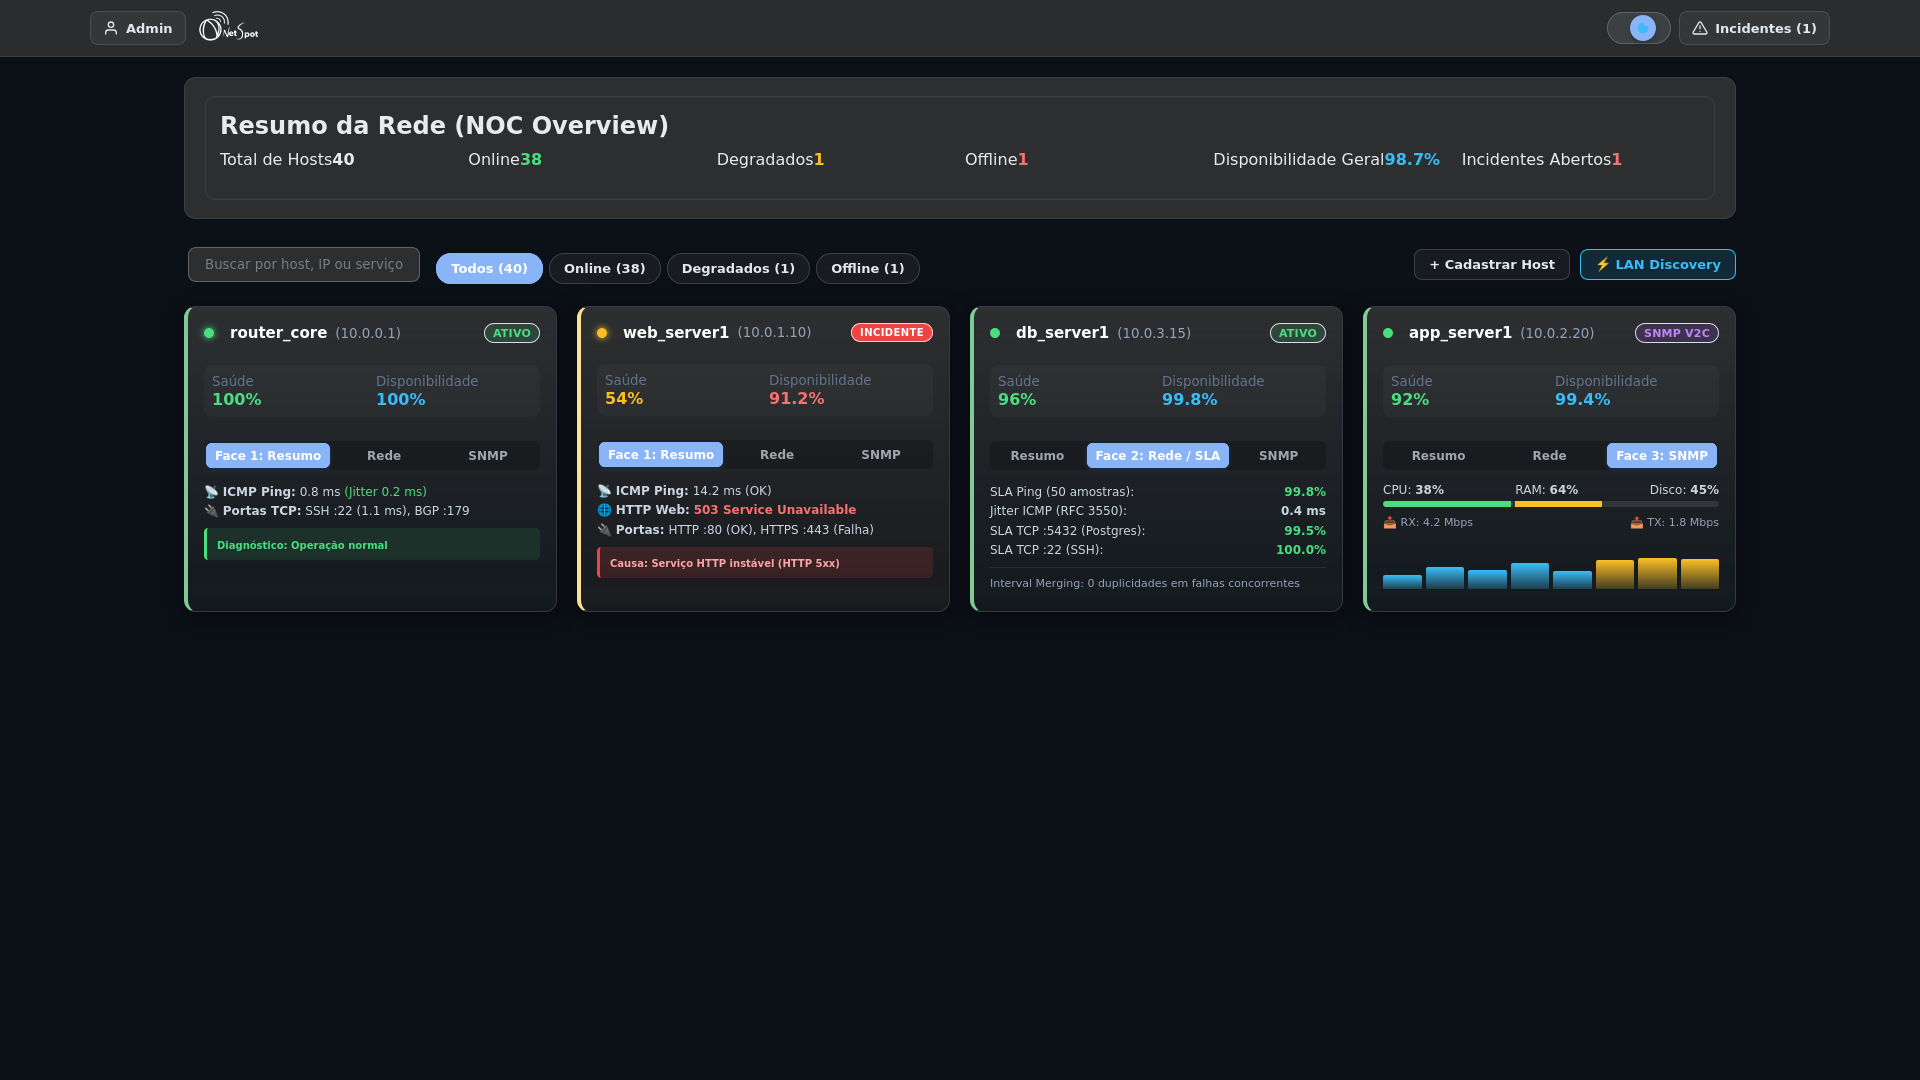
\includegraphics[width=0.98\textwidth]{painel_dashboard.png}
\fonte{Autoria própria (2026).}
\end{figure}

\subsubsection{Engenharia de Performance: Atualização Cirúrgica do DOM, Remoção Otimista e Polling Adaptativo}
A aplicação emprega técnicas avançadas de engenharia de software para conciliar atualizações em tempo real com máxima economia de recursos no cliente e no servidor:
\begin{itemize}[leftmargin=1.25cm]
\item \textbf{Atualização Cirúrgica do DOM em Tempo Real (\texttt{updateHostCardInPlace})}: Um dos desafios centrais no desenvolvimento de SPAs de alta frequência sem frameworks pesados (como React ou Angular) reside em atualizar dados a cada 10 segundos sem incorrer na destruição e recriação do HTML via \texttt{innerHTML}. A recriação cega provocaria tremor visual perceptível (\textit{flickering}), perda de foco de seleção e, criticamente, destruiria os contextos de renderização 2D/Canvas dos gráficos Chart.js e reiniciaria a rotação 3D dos cartões. Para solucionar essa restrição, o método \texttt{updateHostCardInPlace()} realiza mutações atômicas pontuais:
  \begin{enumerate}
  \item Lê e preserva o estado da face atualmente inspecionada pelo operador (\texttt{card.dataset.face}), assegurando que um cartão aberto na Face 2 (SLA) ou Face 3 (SNMP) permaneça estático sem alternar bruscamente para a Face 1;
  \item Altera cirurgicamente as classes CSS do indicador luminoso pulsante (\texttt{status-indicator}) e da flag operacional (\texttt{host-monitor-flag});
  \item Atualiza ou injeta dinamicamente o selo de incidente aberto (\texttt{incident-badge}) apenas quando houver transição de estado, sem desmontar o nó pai;
  \item Atualiza textualmente os medidores de latência, jitter e códigos HTTP, mantendo a árvore do DOM estável com tempo de processamento inferior a 5 milissegundos por ciclo de telemetria.
  \end{enumerate}
\item \textbf{Gerenciamento de Ciclo de Vida do Chart.js e Prevenção de Vazamento de Memória}: Na Face 3 e nos modais de telemetria histórica, os gráficos de CPU, RAM, Disco e Tráfego de Rede são renderizados pela biblioteca Chart.js. Para prevenir vazamento de memória (\textit{memory leaks}) no motor V8 do navegador decorrente de instâncias órfãs de canvas, o sistema mantém um registro global indexado de instâncias ativas (\texttt{window.chartInstances}). Antes de cada nova renderização ou redimensionamento de janela, a instância prévia vinculada ao elemento \texttt{<canvas>} é explicitamente desvinculada e destruída através do método \texttt{chart.destroy()}, liberando os contextos de renderização gráfica.
\item \textbf{Remoção Otimista (\textit{Optimistic UI})}: Ao solicitar a exclusão de um host, a interface aplica instantaneamente uma transição de desvanecimento CSS (\textit{fade-out}) de 200 ms e remove o cartão do DOM, recalculando paralelamente os totais do painel de resumo superior antes mesmo da confirmação da requisição pela API. Em caso improvável de falha na requisição, o estado visual é restaurado com notificação de erro (\textit{Toast});
\item \textbf{Lixeira Lógica (\textit{Soft Delete})}: A exclusão move o registro para a lixeira mediante carimbo na coluna \texttt{deleted\_at}. Um modal dedicado (\texttt{trashModal}) permite consultar os ativos excluídos, restaurá-los com restauração imediata do histórico ou executar a remoção definitiva do banco de dados;
\item \textbf{Polling Adaptativo Bi-Modal}: Para conciliar dados em tempo real com economia de processamento no cliente e no servidor, o script \texttt{app.js} monitora a visibilidade da aba do navegador via \texttt{document.hidden}:
  \begin{itemize}
  \item \textit{Aba Visível (Foreground)}: Ciclo rápido com \textit{Light Refresh} a cada 10 segundos (status rápidos, alertas e resumo) e \textit{Heavy Refresh} a cada 10 segundos (métricas analíticas completas);
  \item \textit{Aba Oculta (Background)}: Ciclo reduzido com consultas leves a cada 30 segundos e consultas pesadas a cada 120 segundos, poupando ciclos de CPU, bateria e consumo de banda;
  \end{itemize}
\item \textbf{Proteção contra Interrupções de UI}: O motor de atualização detecta interações ativas do usuário (digitação em campos de entrada) ou modais abertos no DOM, postergando atualizações pesadas para evitar perda de foco ou alterações inesperadas no formulário.
\end{itemize}

\subsubsection{Acessibilidade Digital (WCAG 2.1 AA) e Usabilidade Ergonômica}
Com o propósito de atender às diretrizes internacionais de acessibilidade na web (\textit{Web Content Accessibility Guidelines} -- WCAG 2.1 nível AA \cite{w3c2018wcag21}) e oferecer conforto visual e cognitivo aos operadores, a interface do NetSpot incorpora os seguintes padrões de engenharia de front-end:
\begin{itemize}[leftmargin=1.25cm]
\item \textbf{Relação de Contraste Cromático}: Tanto no tema escuro quanto no tema claro, a paleta de cores assegura uma taxa de contraste superior ao limiar mínimo de 4.5:1 exigido pela WCAG para textos e elementos interativos normais (alcançando marcas de 5.6:1 e superiores nos selos de status, métricas numéricas e tipografia secundária);
\item \textbf{Navegação Teclado-Cêntrica e Foco Visível}: Todos os elementos interativos (links, botões, campos de entrada e seletores) contam com indicadores de foco customizados de alta visibilidade através do pseudo-seletor CSS \texttt{:focus-visible} com contorno em ciano vívido (\texttt{\#38bdf8}), viabilizando operação ágil e completa do painel sem necessidade de dispositivo apontador (mouse);
\item \textbf{Confinamento de Foco em Diálogos Modais (\textit{Focus Trap})}: Os modais de edição, cadastro, histórico, descoberta e lixeira implementam interceptação programática do foco por JavaScript. Ao abrir uma janela sobreposta, o foco é transferido automaticamente ao primeiro elemento acionável e mantido em laço fechado durante a navegação pela tecla \texttt{Tab}, prevenindo dispersão para elementos ocultos ao fundo. O fechamento é suportado universalmente pela tecla \texttt{Escape}, restaurando o foco ao botão de origem;
\item \textbf{Semântica ARIA e Rótulos Descritivos}: A árvore de acessibilidade é enriquecida com atributos WAI-ARIA (\texttt{aria-label}, \texttt{aria-hidden}, \texttt{role='dialog'} e \texttt{aria-live}), garantindo que leitores de tela interpretem adequadamente transições de status, botões de ícone puro e gráficos vetoriais;
\item \textbf{Ergonomia dos Cartões 3D e Indicadores de Estado}: Cada cartão de host dispõe de um indicador numérico sutil de face ativa (\texttt{1/3}, \texttt{2/3} e \texttt{3/3}), acompanhado de dicas de contexto (\textit{tooltips}) e botões de paginação dedicados, eliminando a ambiguidade visual durante rotações tridimensionais;
\item \textbf{Ações em Massa e Proteção contra Exclusão Involuntária}: O módulo de Descoberta de Rede disponibiliza botões ergonômicos de seleção e desmarcação global (\textit{Selecionar Todos} e \textit{Desmarcar Todos}), enquanto a lixeira de ativos conta com diálogo secundário de confirmação de segurança antes da execução do expurgo definitivo, prevenindo perda acidental de dados.
\end{itemize}

\subsubsection{Central de Gestão de Incidentes (\texttt{incidents.html})}
A plataforma possui uma página dedicada à operação formal de incidentes do NOC (\texttt{Frontend/incidents.html}). O painel provê busca rápida por ativo, exibindo uma \textit{timeline} completa dos eventos com:
\begin{itemize}[leftmargin=1.25cm]
\item Nome do host e severidade da falha;
\item Causa identificada pelo motor heurístico;
\item Horário de início da anomalia e horário de encerramento;
\item Duração total da indisponibilidade em minutos/segundos para análise de MTTR;
\item Emissão de notificações sonoras e visuais nativas do navegador através da Web Notifications API (\texttt{Notification.permission}).
\end{itemize}

A Figura~\ref{fig:painel_incidentes} ilustra a interface dedicada da Central de Incidentes do NetSpot, exibindo o sumário de confiabilidade (MTTR e alertas), os chips de filtragem de estado e a listagem sequencial de falhas ativas e resolvidas com o diagnóstico de causa provável.

\begin{figure}[H]
\centering
\caption{Central de gestão de incidentes do NetSpot com linha do tempo de eventos operacionais e diagnóstico heurístico}
\label{fig:painel_incidentes}
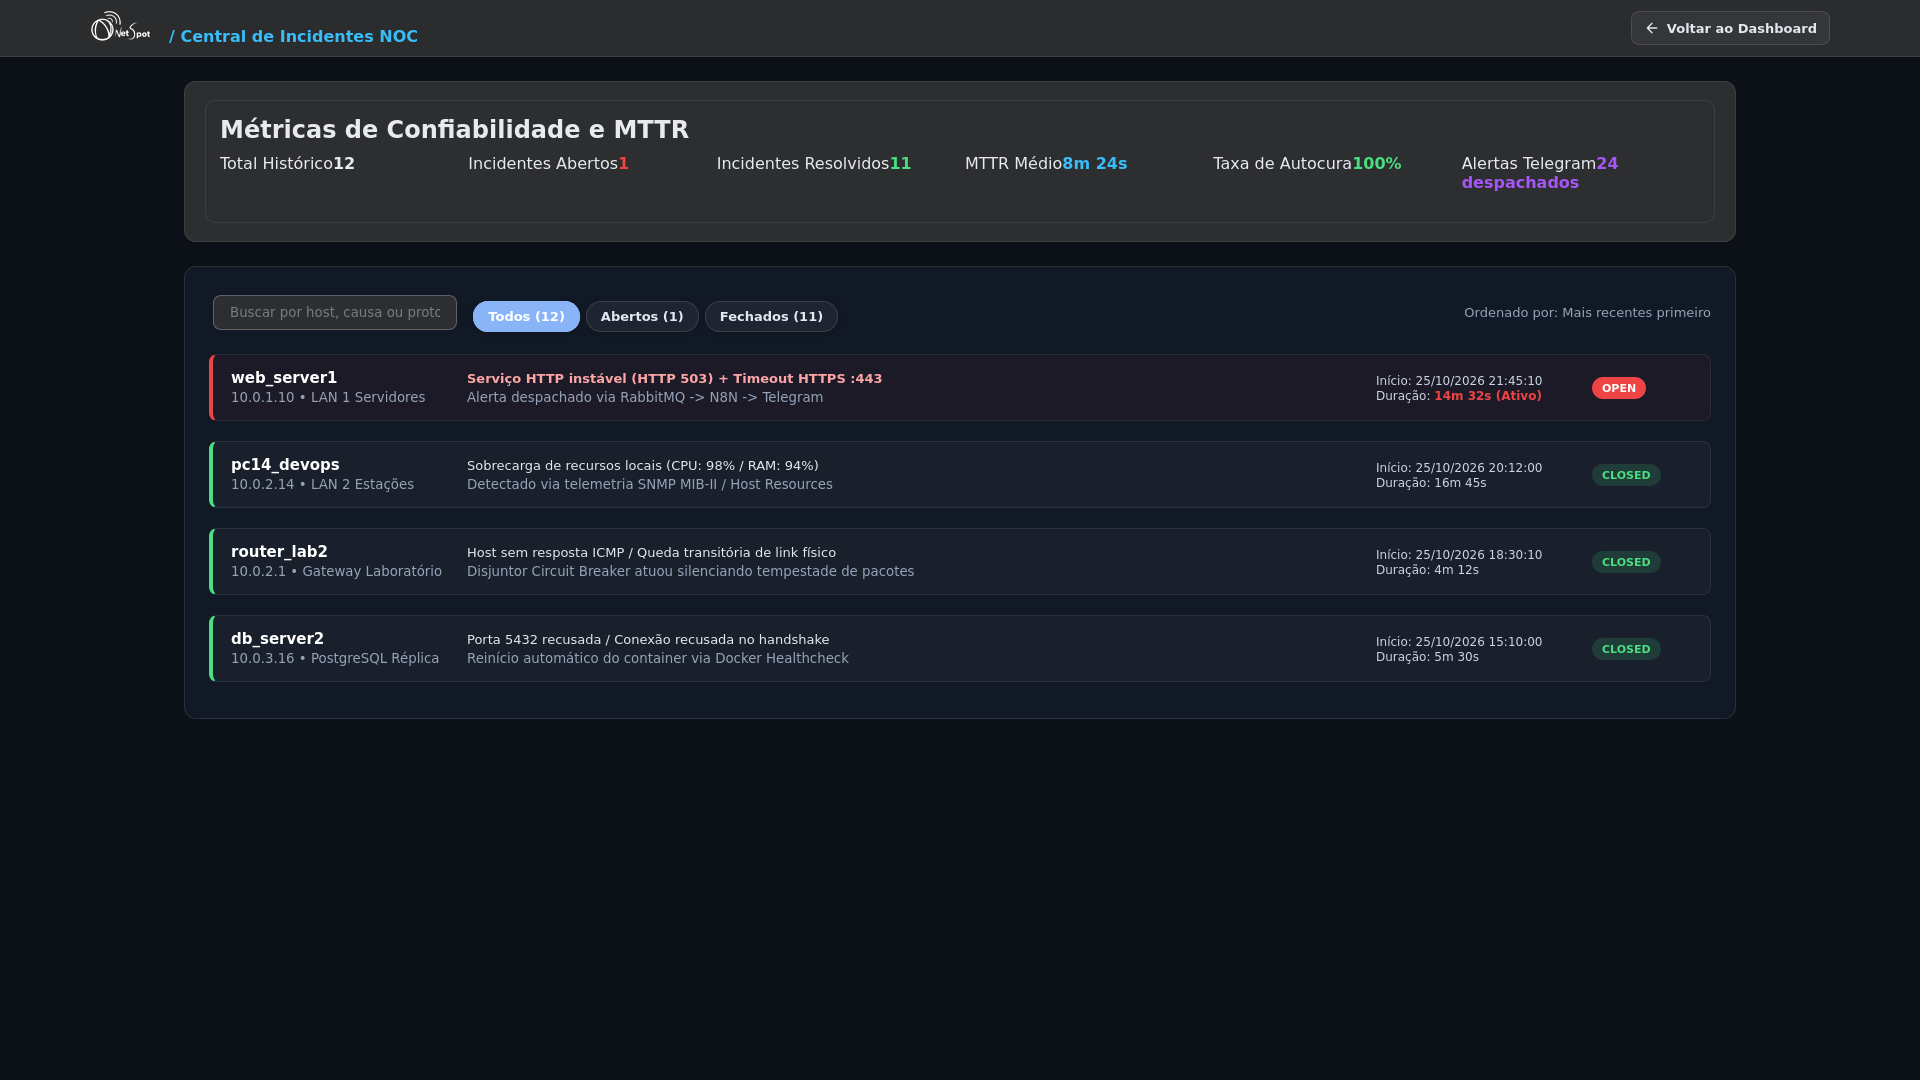
\includegraphics[width=0.98\textwidth]{painel_incidentes.png}
\fonte{Autoria própria (2026).}
\end{figure}

\subsubsection{Camada de Segurança, Sessão, Autenticação JWT e Hardening Web}
O acesso ao sistema é protegido por autenticação baseada em JSON Web Tokens (JWT). As rotas da SPA verificam a existência do token no \texttt{localStorage} antes da renderização de qualquer componente, redirecionando usuários não autenticados para a tela de login (\texttt{login.html}). Todas as chamadas de API são envelopadas pela função utilitária \texttt{fetchWithAuth()}, que injeta o cabeçalho \texttt{Authorization: Bearer <token>} e intercepta erros \texttt{401 Unauthorized}, disparando avisos \textit{Toast} e encerrando a sessão com segurança. No primeiro acesso de um operador com credenciais padrão, o sistema aciona compulsoriamente o modal de troca de senha (\texttt{changePwdModal}) antes de liberar o acesso às funções de monitoramento.

Complementarmente, a camada de apresentação incorpora diretrizes de defesa em profundidade (\textit{Defense in Depth}) recomendadas pelas boas práticas da OWASP:
\begin{itemize}[leftmargin=1.25cm]
\item \textbf{Mitigação de Cross-Site Scripting (XSS)}: Todas as saídas de texto dinâmicas interpoladas no DOM (incluindo nomes de hosts, estados operacionais, tipos de incidente e diagnósticos heurísticos de falha) são processadas por uma rotina de sanitização neutra (\texttt{escapeHtml()}), que converte caracteres especiais de marcação (\texttt{\&}, \texttt{<}, \texttt{>}, \texttt{\textquotedbl}, \texttt{'}) em entidades HTML inócuas, impedindo o sequestro de sessões ou a execução de scripts maliciosos injetados por pacotes de rede adulterados;
\item \textbf{Hardening e Segurança do Servidor Proxy Nginx}: O servidor Nginx Alpine é configurado com cabeçalhos HTTP estritos de proteção contra ataques de sobreposição de quadros (\texttt{X-Frame-Options: SAMEORIGIN}), ataques de farejamento de tipos MIME (\texttt{X-Content-Type-Options: nosniff}), proteção ativa contra XSS no navegador (\texttt{X-XSS-Protection}) e política de referência restritiva (\texttt{Referrer-Policy: strict-origin-when-cross-origin});
\item \textbf{Compactação de Ativos e Bloqueio de Arquivos Internos}: A entrega de ativos estáticos (HTML, CSS, JavaScript e SVG) emprega compactação assíncrona \textit{gzip} (nível 6), minimizando a latência de transferência na rede local. Ademais, o servidor bloqueia estritamente com código HTTP 404 qualquer tentativa de acesso direto a arquivos de infraestrutura e variáveis de ambiente (como \texttt{Dockerfile}, \texttt{nginx.conf} e arquivos ocultos do ecossistema Docker).
\end{itemize}

\section{AMBIENTE DE EXPERIMENTAÇÃO E RESULTADOS}
A validação técnica do NetSpot foi conduzida em três frentes complementares: simulação em ambiente virtualizado de larga escala com o framework Kathará (abrangendo a topologia padrão de 40 nós e a topologia de estresse em alta densidade com 126 nós monitorados), validação em ambiente físico real realizada no Laboratório 2 do prédio do Ensino Superior do IFNMG -- Campus Januária, e verificação formal de código através de uma suíte exaustiva de 86 testes automatizados via Pytest.

\subsection{LABORATÓRIO DE SIMULAÇÃO KATHARÁ}
Para avaliar a escalabilidade, a estabilidade sob carga e o comportamento dos mecanismos de resiliência em topologias complexas com saltos múltiplos de roteamento, foi projetado e executado um laboratório de emulação de larga escala utilizando o framework Kathará \cite{bonola2018kathara}, configurado no arquivo \texttt{lab.conf}.

O ambiente emula um total de 47 dispositivos de rede interconectados, dos quais 40 são nós finais monitorados ativamente (30 estações de trabalho e 10 servidores dedicados de serviços), operando sobre 4 roteadores intermediários e 3 switches de agregação com comutação de camada 2, cuja topologia lógica está ilustrada na Figura \ref{fig:laboratorio_kathara}:

\begin{figure}[H]
\centering
\caption{Topologia do ambiente de laboratório simulado em Kathará}
\label{fig:laboratorio_kathara}
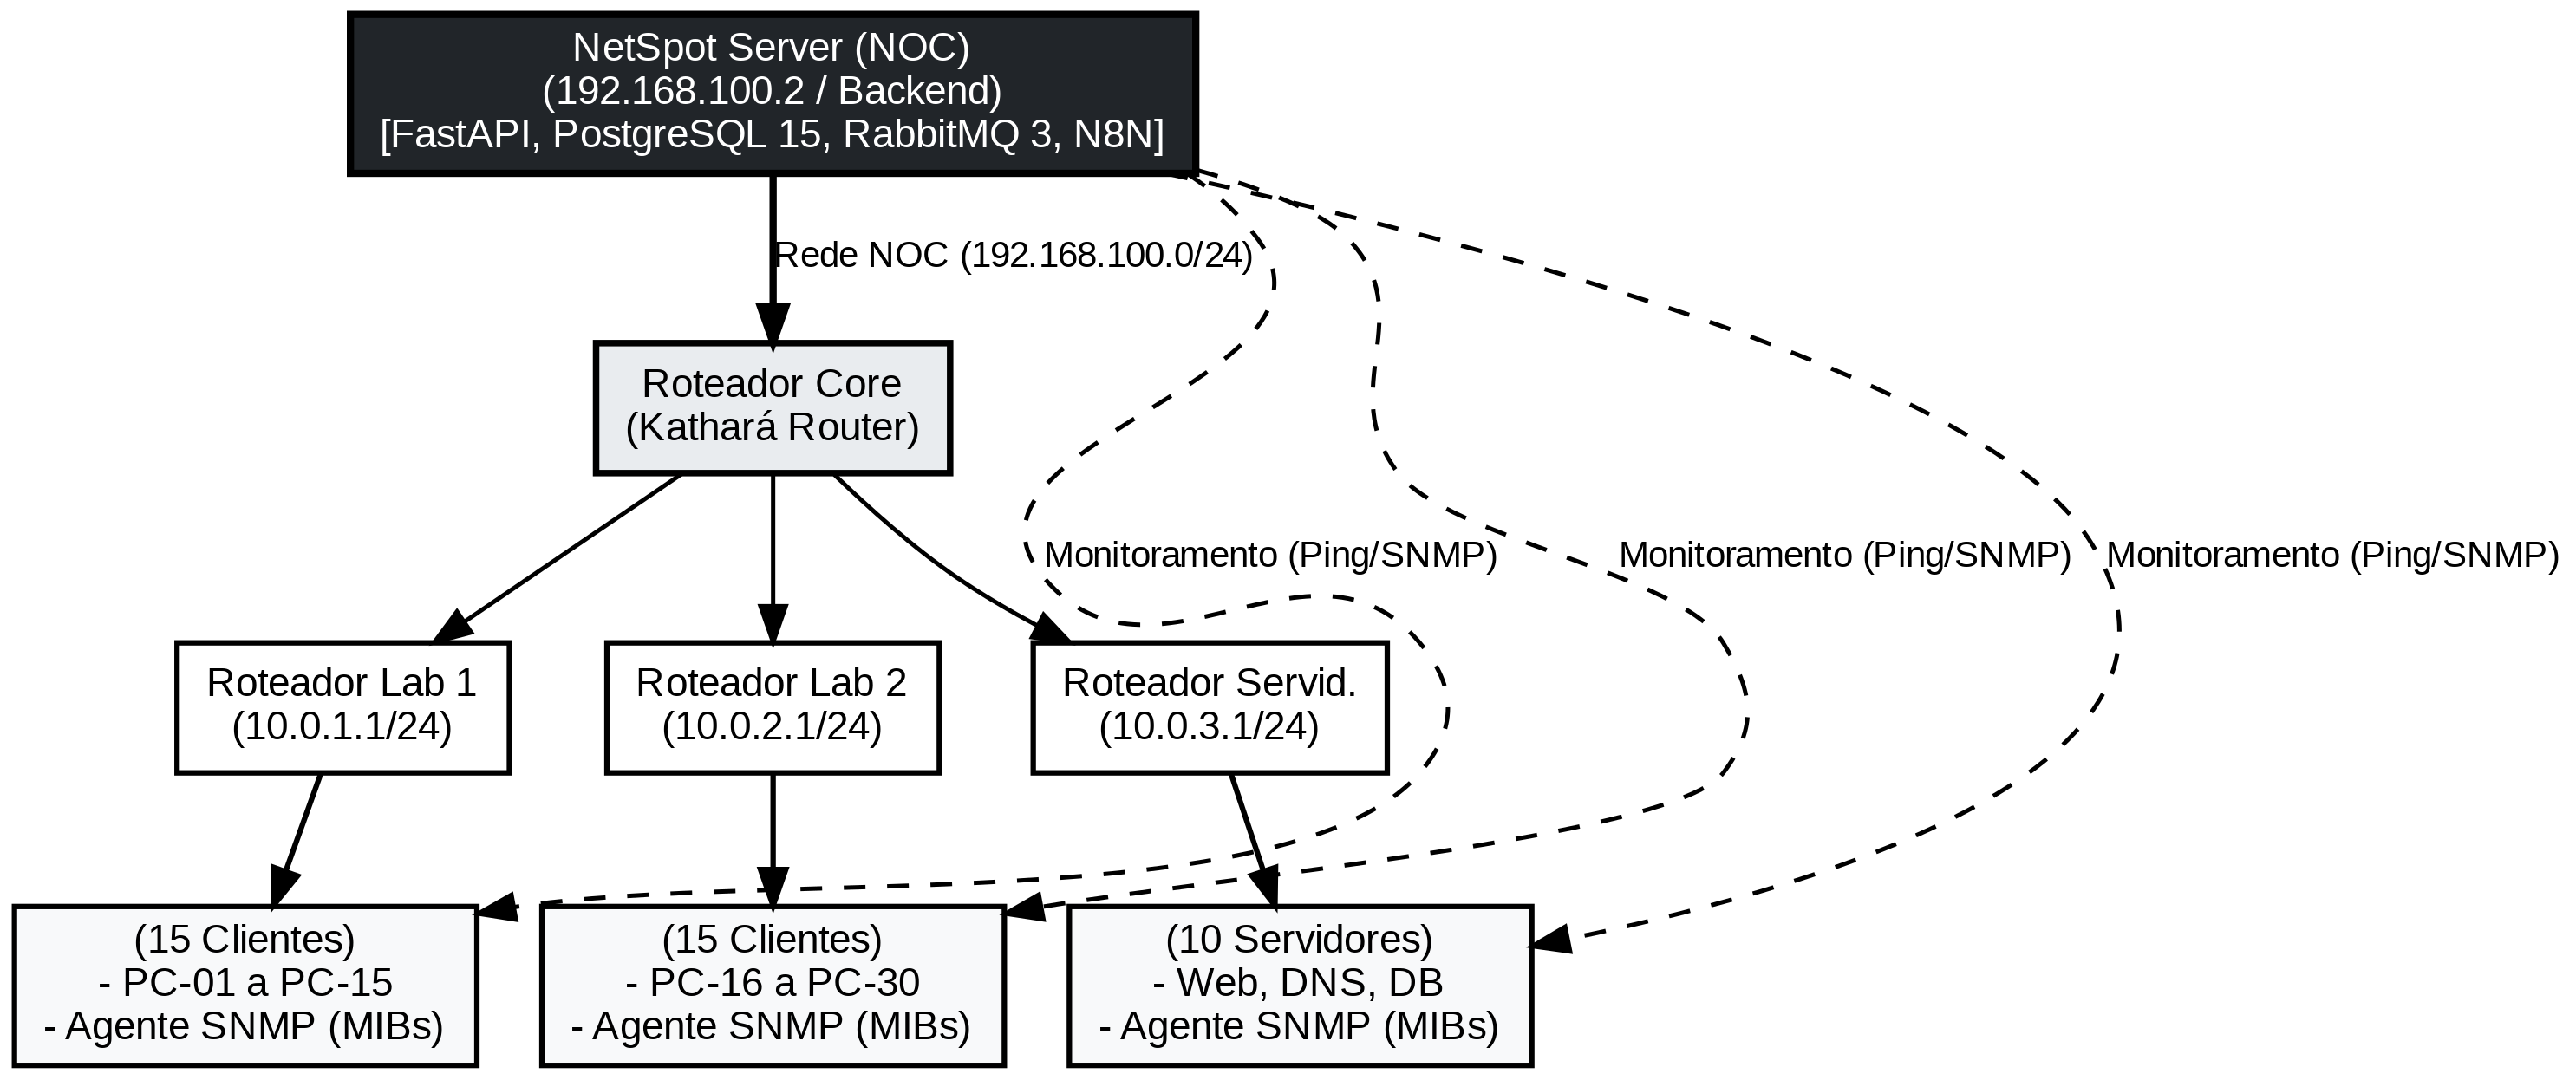
\includegraphics[width=0.92\textwidth]{laboratorio_kathara.png}
\fonte{Autoria própria (2026).}
\end{figure}

A arquitetura de interconexão e roteamento do laboratório foi desenhada com alto realismo:
\begin{itemize}[leftmargin=1.25cm]
\item \textbf{Roteador Central de Núcleo (\texttt{router\_core})}: Possui uma interface em ponte (\textit{bridged}) vinculada à interface de rede do servidor NetSpot, recebendo endereço IP por DHCP e atuando como gateway institucional. Implementa encaminhamento de pacotes IPv4 (\texttt{net.ipv4.ip\_forward=1}) e tradução de endereços de saída (\textit{Source NAT}) via \texttt{iptables -t nat -A POSTROUTING -o eth4 -j MASQUERADE}. É interligado aos três roteadores de laboratório por enlaces dedicados ponto a ponto (\texttt{100.0.1.254/24}, \texttt{100.0.2.254/24} e \texttt{100.0.3.254/24}), roteando o tráfego estático para as respectivas sub-redes;
\item \textbf{Roteadores de Laboratório (\texttt{router\_lab1}, \texttt{router\_lab2}, \texttt{router\_lab3})}: Executam instâncias Linux roteando pacotes entre a malha central e as sub-redes locais dos laboratórios (\texttt{10.0.1.0/24}, \texttt{10.0.2.0/24} e \texttt{10.0.3.0/24}), com rotas padrão apontadas para o \texttt{router\_core} e daemons de agente SNMP ativos;
\item \textbf{Comutadores de Enlace (\texttt{switch\_lab1}, \texttt{switch\_lab2}, \texttt{switch\_lab3})}: Configurados como pontes virtuais Ethernet nativas (\textit{Linux Bridges}) através do utilitário \texttt{brctl}, agregando até 15 portas físicas lógicas por comutador com protocolo Spanning Tree ativado (\texttt{brctl stp on}) para prevenção contra tempestades de broadcast decorrentes de loops de comutação.
\end{itemize}

A caracterização funcional e o mapeamento de endereçamento das sub-redes configuradas no ambiente Kathará estão descritos na Tabela \ref{tab:distribuicao_kathara}:

\begin{table}[H]
\centering
\caption{Distribuição de nós no ambiente de laboratório Kathará}
\label{tab:distribuicao_kathara}
\small
\begin{tabular}{@{}p{4.5cm}p{4.0cm}p{6.5cm}@{}}
\toprule
\textbf{Sub-rede} & \textbf{Faixa IP} & \textbf{Descrição dos Ativos e Serviços} \\
\midrule
Rede de Servidores (LAN 1) & \texttt{10.0.1.0/24} & Servidores HTTP (Nginx/Apache), PostgreSQL, DNS (Bind9) e SSH \\
Rede de Clientes (LAN 2) & \texttt{10.0.2.0/24} & Estações de trabalho Linux e Windows com agentes SNMP nativos \\
Rede de Infraestrutura (LAN 3) & \texttt{10.0.3.0/24} & Roteadores virtuais FRRouting e Switches gerenciáveis \\
Rede de Gestão NOC (LAN 4) & \texttt{192.168.100.0/24} & Servidor NetSpot (FastAPI, RabbitMQ, PostgreSQL, N8N, Frontend) \\
\bottomrule
\end{tabular}
\fonte{Autoria própria (2026).}
\end{table}

\subsubsection{Cenário de Estresse e Escalabilidade em Alta Densidade (126 Hosts em 10.0.0.0/22)}
Para submeter o motor assíncrono ao limite de capacidade projetado para ambientes de médio porte, foi concebido o cenário escalado de estresse (\texttt{Teste - Kathará/Lab-126hosts/}). O ambiente agrega um bloco CIDR \texttt{10.0.0.0/22} com **126 nós monitorados simultaneamente** em três domínios de broadcast:
\begin{itemize}[leftmargin=1.25cm]
\item \textbf{Sub-rede 1 (Acadêmica e DevOps -- \texttt{10.0.1.0/24}, 47 nós)}: Roteador \texttt{router\_lab1} (10.0.1.1) interligando 26 estações acadêmicas, 12 servidores DevOps (SSH :22 e HTTP :8080) e 8 estações administrativas com agentes SNMP ativos;
\item \textbf{Sub-rede 2 (Engenharia e Full-Stack -- \texttt{10.0.2.0/24}, 47 nós)}: Roteador \texttt{router\_lab2} (10.0.2.1) conectando 26 nós de desenvolvimento, 12 servidores de aplicação web (Node.js :3000) e 8 servidores de banco de dados relacional (PostgreSQL :5432);
\item \textbf{Sub-rede 3 (Data Center Corporativo -- \texttt{10.0.3.0/24}, 32 nós)}: Roteador \texttt{router\_lab3} (10.0.3.1) e 31 servidores dedicados (9 servidores Web Apache :80/:443, 6 instâncias de aplicação Tomcat :8080, 6 instâncias de banco de dados, 4 servidores DNS Bind9 com zonas diretas e reversas completas \texttt{db.10.0.1..3}, 3 servidores de cache Redis e 3 balanceadores Nginx).
\end{itemize}

O motor assíncrono concluiu a rodada completa de sondagens multicamada (ICMP, TCP e telemetria SNMP) sobre os 126 hosts em apenas **1.22 segundos**, mantendo folga operacional de 87\% dentro da janela estrita de 10 segundos do ciclo.

No laboratório, foram injetadas anomalias intencionais utilizando as ferramentas de estresse de rede e sistema:
\begin{itemize}[leftmargin=1.25cm]
\item \texttt{tc} (\textit{Traffic Control}): Simulação de alta latência (250 ms $\pm$ 50 ms de \textit{jitter}) e taxa de descarte de pacotes de 15\% nas interfaces de enlace da LAN 1 e LAN 2;
\item \texttt{stress-ng}: Injeção de 100\% de utilização de CPU e 90\% de saturação de memória RAM nas estações de trabalho monitoradas por SNMP;
\item Queda abrupta de interfaces (\texttt{ip link set dev eth0 down}) para simular interrupções de links físicos.
\end{itemize}

O NetSpot identificou todas as oscilações de conectividade em tempo médio inferior a 20 segundos. Nos hosts que sofreram indisponibilidade total, o padrão \textit{Circuit Breaker} transitou para o estado \texttt{OPEN} pontualmente após a 5ª falha sucessiva, interrompendo o envio de pacotes adicionais e protegendo os enlaces contra saturação desnecessária. Não houve perda de eventos de alerta graças ao encaminhamento seguro via \textit{Dead Letter Queue} (DLQ), e os alertas foram entregues de forma desduplicada no Telegram.

\subsection{VALIDAÇÃO EM AMBIENTE FÍSICO REAL (IFNMG -- CAMPUS JANUÁRIA)}
Para atestar a viabilidade prática da solução fora de ambientes puramente simulados, o NetSpot foi implantado e executado em condições reais de infraestrutura no Laboratório 2 do prédio do Ensino Superior do IFNMG -- Campus Januária.

Importa destacar que um dos desafios mais expressivos de ordem prática e metodológica vivenciados durante a condução desta pesquisa residiu na obtenção de uma quantidade considerável e simultânea de computadores físicos para a execução contínua de baterias de testes de estresse de rede. Os laboratórios de informática da instituição de ensino possuem uma intensa e ininterrupta grade horária de atividades pedagógicas voltadas às aulas dos cursos de graduação e técnicos. Consequentemente, a mobilização exclusiva de dezenas de máquinas físicas por períodos prolongados -- com permissões para desativação temporária de mecanismos de proteção, alteração de regras locais de firewall, injeção de perturbações de tráfego e simulações de sobrecarga de hardware -- revelou-se operacionalmente restrita para evitar qualquer interferência nas atividades regulares da comunidade acadêmica.

Essa contingência da infraestrutura real fundamentou e justificou plenamente a concepção da estratégia metodológica híbrida adotada neste trabalho: combinou-se o rigor experimental em larga escala alcançado no ambiente virtualizado com o framework Kathará (onde mais de 40 nós virtuais roteados puderam ser severamente estressados sem riscos operacionais) com a validação física direta nas estações de trabalho reais do Laboratório 2 durante os intervalos programados de disponibilidade das máquinas.

O ambiente físico de experimentação compreendeu computadores de mesa do laboratório conectados à rede local institucional, operando em arquitetura heterogênea sob os sistemas operacionais Ubuntu Linux 22.04 LTS e Microsoft Windows 10/11 Pro. Foram devidamente parametrizados os serviços de agente SNMP nativos em cada ecossistema: o pacote \texttt{snmpd} (\textit{Net-SNMP}) no Linux e o recurso nativo de SNMP do Windows vinculado à comunidade de leitura padronizada \texttt{netspot}.

O NetSpot executou com sucesso a rotina de varredura automática de rede (\texttt{LAN Discovery}) sobre a sub-rede dos laboratórios de ensino superior, detectando os nós físicos e integrando-os de forma imediata ao painel SPA. Durante os testes práticos de desconexão física de cabos de rede (simulando perda de portadora física) e derrubada controlada de instâncias locais de serviços web, o sistema identificou os incidentes em tempo real, rebaixou o \textit{Health Score} instantaneamente para níveis críticos e encaminhou os alertas estruturados para o canal do Telegram via N8N, atestando a tolerância a falhas e a aplicabilidade da ferramenta em infraestruturas reais de ensino.

\subsection{SUÍTE DE TESTES AUTOMATIZADOS (PYTEST)}
A integridade das regras de negócio, a consistência dos algoritmos matemáticos e a segurança dos microsserviços foram formalmente validadas através de uma suíte composta por 86 testes automatizados desenvolvidos com a biblioteca Pytest (\texttt{Backend/tests/}), cobrindo tanto testes de unidade analíticos quanto testes de integração assíncronos e auditoria estrita de regressões de segurança. Os resultados estão sintetizados na Tabela \ref{tab:resumo_testes}:

\begin{table}[H]
\centering
\caption{Resumo da suíte de 86 testes automatizados do NetSpot (Pytest)}
\label{tab:resumo_testes}
\small
\begin{tabular}{@{}p{5.0cm}p{7.8cm}p{2.2cm}@{}}
\toprule
\textbf{Módulo de Teste} & \textbf{Escopo de Validação Técnica e Contratos Auditados} & \textbf{Resultado} \\
\midrule
\texttt{test\_audit\_regressions.py} & 42 testes de regressões críticas: limite 72b no bcrypt, RLS, RBAC em exclusão, anti-flapping composto, latência 0.0 ms no health e blindagem XSS & 100\% PASSED (42/42) \\
\texttt{test\_checker.py} & 12 testes: checadores concorrentes de ICMP Ping, portas TCP, requisições HTTP/HTTPS e DNS & 100\% PASSED (12/12) \\
\texttt{test\_metrics.py} & 9 testes: algoritmos de Health Score, SLA via Interval Merging, Jitter RFC 3550 e OLS & 100\% PASSED (9/9) \\
\texttt{test\_self\_healing.py} & 8 testes: estados do Circuit Breaker (CLOSED/OPEN/HALF-OPEN), reconexão e DLQ & 100\% PASSED (8/8) \\
\texttt{test\_snmp.py} & 8 testes: resolução polimórfica de OIDs (Linux/Windows), fallback e cache & 100\% PASSED (8/8) \\
\texttt{test\_alert\_logic.py} & 7 testes: 7 heurísticas de causa provável, supressão de firewall e anti-flapping & 100\% PASSED (7/7) \\
\texttt{test\_retention.py} & 3 testes: regras de política de retenção e expurgo temporal de métricas & 100\% PASSED (3/3) \\
\texttt{test\_api\_routes.py} & 3 testes: endpoints RESTful de ingestão, CRUD de hosts e rota \texttt{/healthz} & 100\% PASSED (3/3) \\
\texttt{test\_models\_schemas.py} & 2 testes: validação de entidades ORM SQLAlchemy e esquemas Pydantic & 100\% PASSED (2/2) \\
\midrule
\textbf{TOTAL CONSOLIDADO} & \textbf{Suíte completa sem regressões (execução média em $\sim$6.5 segundos)} & \textbf{100\% PASSED (86/86)} \\
\bottomrule
\end{tabular}
\fonte{Autoria própria (2026).}
\end{table}

A execução da suíte obteve \textbf{100\% de aprovação (86/86 PASSED)}, confirmando a conformidade dos contratos formais de operação, a ausência de regressões lógicas e a confiabilidade de toda a arquitetura assíncrona.

\subsection{CONSUMO DE RECURSOS E DESEMPENHO}
Durante a execução contínua no laboratório Kathará (mais de 40 nós virtuais no cenário padrão e 126 nós no cenário escalado) e na infraestrutura física do IFNMG, o consumo de recursos computacionais do servidor de monitoramento foi mensurado utilizando ferramentas de telemetria do sistema operacional (\texttt{docker stats} e \texttt{htop}):

\begin{itemize}[leftmargin=1.25cm]
\item \textbf{Utilização de CPU}: O motor assíncrono em Python 3.11, operando em conjunto com o barramento RabbitMQ e o Nginx, manteve consumo médio de CPU inferior a 4.2\%, atingindo picos máximos de apenas 7.8\% durante ciclos concorrentes de varredura de sub-rede e apenas 12.0\% durante o ciclo completo de 126 nós no Kathará.
\item \textbf{Ocupação de Memória RAM}: O conjunto completo dos 5 microsserviços Docker manteve alocação estável de memória na faixa dos 580 MB, distribuídos entre o PostgreSQL (~180 MB), RabbitMQ (~160 MB), FastAPI (~120 MB), N8N (~100 MB) e Nginx (~20 MB).
\item \textbf{Tempo de Detecção e Alerta}: O tempo médio transcorrido entre a ocorrência de uma anomalia em um host e a entrega da notificação formatada no Telegram foi de 18.4 segundos.
\end{itemize}

É importante ressaltar que ferramentas consolidadas de mercado, tais como o Zabbix \cite{zabbix2026manuals} e o Prometheus \cite{prometheus2026overview}, são amplamente reconhecidas pela indústria por sua maturidade e alta eficiência computacional no nível de máquina, sendo implementadas em linguagens compiladas de baixo nível e alto desempenho (C e Go, respectivamente). Todavia, no contexto de pequenas e médias empresas e instituições de ensino sem equipes de TI dedicadas exclusivamente a operações de rede, a principal barreira operacional imposta por essas plataformas não reside no consumo de processamento ou memória, mas sim na sua \textbf{elevada complexidade de instalação inicial, parametrização e manutenção contínua}:
\begin{itemize}[leftmargin=1.25cm]
\item \textbf{Zabbix}: Exige o provisionamento e dimensionamento manual de um SGBD relacional dedicado (PostgreSQL ou MySQL), parametrização de particionamento e esquemas de dados, instalação e configuração manual de agentes em cada nó monitorado, além de gerenciamento exaustivo de macros, triggers e templates de MIBs heterogêneas;
\item \textbf{Prometheus}: Opera como um ecossistema desacoplado que requer a orquestração e manutenção de múltiplos daemons independentes (Prometheus Server, Alertmanager, Grafana para exibição visual de dashboards, além de coletores auxiliares como \texttt{node\_exporter} e \texttt{snmp\_exporter}), demandando a geração prévia de arquivos de MIB compilados e o domínio da linguagem de consulta PromQL para criação de alertas e painéis;
\item \textbf{NetSpot (NOC Lite)}: Adota o paradigma \textit{turn-key} completamente integrado via Docker Compose, disponibilizando em um único comando de subida o banco relacional pré-configurado, barramento AMQP, fluxos de automação N8N pré-definidos com templates para o Telegram, rotinas de descoberta visual de sub-redes e interface SPA moderna com cartões 3D, eliminando a edição manual de arquivos estáticos de configuração ou o domínio de linguagens proprietárias de consulta.
\end{itemize}

O comparativo de perfil operacional e esforço de manutenção entre o NetSpot e as ferramentas corporativas tradicionais é sintetizado na Tabela \ref{tab:comparativo_requisitos}:

\begin{table}[H]
\centering
\caption{Comparativo de perfil operacional e esforço de manutenção entre abordagens de monitoramento}
\label{tab:comparativo_requisitos}
\small
\begin{tabular}{@{}p{3.5cm}p{5.5cm}p{5.7cm}@{}}
\toprule
\textbf{Critério Operacional} & \textbf{Abordagem NOC Lite (NetSpot)} & \textbf{Sistemas Tradicionais (Zabbix / Prometheus)} \\
\midrule
Foco de Operação & Praticidade, visualização ágil e detecção preventiva & Telemetria massiva e observabilidade altamente customizada \\
Esforço de Instalação & \textit{Turn-key} em comando único via contêineres (\texttt{docker compose}) & Elevado: provisionamento manual de SGBD, múltiplos daemons e agentes \\
Manutenção Contínua & Baixa: descoberta visual de rede e configuração 100\% via web & Contínua: edição de arquivos YAML, compilação de MIBs e templates \\
Curva de Aprendizado & Baixa: painel intuitivo acessível a técnicos generalistas & Íngreme: exige domínio de PromQL, macros, triggers e arquitetura \\
Stack de Visualização & Nativa e integrada (SPA responsiva com cartões 3D) & Exige ferramentas desacopladas (Zabbix Frontend ou Grafana) \\
Eficiência Computacional & Leve ($<$ 600 MB de RAM e CPU $<$ 5\%), execução local & Altamente eficiente e leve (C/Go), porém com pilha multi-serviços \\
Público e Cenário-Alvo & PMEs, laboratórios de ensino e redes locais enxutas & Grandes \textit{datacenters}, nuvem massiva e provedores (ISPs) \\
\bottomrule
\end{tabular}
\fonte{Autoria própria (2026).}
\end{table}

Estes resultados experimentais comprovam que o NetSpot atende integralmente à hipótese de pesquisa, viabilizando monitoramento proativo com simplificação operacional drástica em ambientes convencionais, sem impor custos de manutenção especializados à infraestrutura de TIC.

\section{CONSIDERAÇÕES FINAIS}
O desenvolvimento e a validação do \textbf{NetSpot (NOC Lite)} demonstraram a plena viabilidade técnica de conceber um sistema completo de monitoramento, observabilidade e prevenção de falhas em redes de computadores, priorizando a simplicidade operacional, a praticidade de uso e o baixo custo computacional.

A fundamentação da modelagem orientada a objetos na metodologia de \citeonline{wazlawick2011analise}, articulada à Arquitetura Orientada a Eventos (EDA), ao motor assíncrono em Python (3.11/3.12), ao barramento RabbitMQ com tolerância a falhas via \textit{Dead Letter Queue} e aos mecanismos de resiliência (\textit{Circuit Breaker}, autocura de pools, \textit{Anti-Flapping} composto e \textit{Graceful Shutdown}), comprovou ser altamente eficiente para eliminar gargalos de I/O, prevenir tempestades de pacotes e garantir zero perda de eventos. A modelagem orientada a objetos das entidades de domínio e classes de serviço, associada à rica interface web SPA com design \textit{Dark and White}, cartões 3D com 3 faces de telemetria, modo Tabela NOC de alta densidade e conformidade de acessibilidade digital (WCAG 2.1 AA), conferiu ao operador uma experiência de uso ágil e ergonômica, dispensando parametrizações complexas.

A eficácia do sistema foi validada empiricamente através de dois cenários de larga escala simulados no Kathará (topologia padrão com 40 nós roteados e topologia escalada de estresse com 126 nós monitorados em alta densidade sob rede \texttt{10.0.0.0/22}), complementada pela implantação prática em estações físicas de trabalho reais no Laboratório 2 do IFNMG -- Campus Januária e pela suíte de 86 testes automatizados (100\% de aprovação via Pytest). Em todos os cenários avaliados, o consumo de recursos manteve-se estritamente abaixo do teto de 12\% de CPU e menos de 600 MB de RAM, consolidando o NetSpot como uma ferramenta NOC Lite prática, resiliente e acessível para instituições públicas e organizações de pequeno e médio porte.

Como perspectivas de trabalhos futuros decorrentes das limitações conhecidas do escopo atual, propõe-se:
\begin{enumerate}[leftmargin=1.25cm]
\item O suporte ao protocolo SNMPv3, introduzindo autenticação criptográfica baseada em usuários (USM) e encriptação de dados (SHA/AES);
\item A flexibilização da gestão de credenciais SNMP, possibilitando cadastrar comunidades arbitrárias distintas por dispositivo gerenciado;
\item A implementação de controle de acesso baseado em papéis (\textit{Role-Based Access Control} -- RBAC), estabelecendo perfis granulares para Administradores, Operadores de NOC e Visualizadores;
\item O desenvolvimento de coletores remotos distribuídos (\textit{Distributed Pollers}), permitindo monitorar filiais geodistribuídas sob um único painel centralizado;
\item A incorporação de algoritmos de aprendizado de máquina para predição proativa de saturação de links e esgotamento de armazenamento com base em séries temporais.
\end{enumerate}

\clearpage
\addcontentsline{toc}{section}{REFERÊNCIAS}
\bibliographystyle{abntex2-alf}
\bibliography{referencias}
\end{document}
